\documentclass[twoside,10pt]{article}

\usepackage[margin=1in]{geometry} 
\usepackage{fancyhdr}
%\setlength{\headheight}{15.2pt}
\pagestyle{fancy}
\fancyhf{}

\usepackage{tikz}
\usepackage[framemethod=TiKZ]{mdframed} 
\usepackage{pgfplots}
\pgfplotsset{compat=1.7}
\usetikzlibrary{matrix,calc,patterns,angles,quotes}

\usepackage{amsthm}
\usepackage{amssymb}
\usepackage{amsfonts}
\usepackage{xcolor}
\usepackage{mathtools}
\usepackage{enumerate}
\usepackage{cancel} 
\usepackage{wasysym}

\usepackage{polski}
\usepackage[utf8]{inputenc}
\newcommand{\RR}{\mathbb{R}}
\newcommand{\CC}{\mathbb{C}}
\newcommand{\QQ}{\mathbb{Q}}
\newcommand{\Lin}{\operatorname{Lin}}
\newcommand{\scp}[2]{\left\langle #1, #2 \right\rangle} 
\newcommand{\norm}[1]{\left\lVert#1\right\rVert}
\newcommand{\verteq}{\rotatebox{90}{$=$}}
\newcommand{\vertin}{\rotatebox{90}{$\ni$}} 
\newcommand{\vertle}{\rotatebox{90}{$\le$}} 
\newcommand{\vertge}{\rotatebox{90}{$\ge$}} 
\newcommand{\vertni}{\rotatebox{90}{$\in$}}
\newcommand{\underscript}[3]{\underset{\scriptstyle{\overset{#2}{#3}}}{#1}}
\newcommand{\overscript}[3]{\overset{\scriptstyle{\underset{#2}{#3}}}{#1}}

\definecolor{lightgray}{gray}{0.96}

\setlength\parindent{0pt}

\theoremstyle{definition}
\newmdtheoremenv[nobreak=true]{tw}%
                {Twierdzenie}[section]
                
\theoremstyle{definition}
\newmdtheoremenv[nobreak=true,roundcorner=5pt]{ft}%
                [tw]{Fakt}

\theoremstyle{definition}
\newmdtheoremenv[nobreak=true,leftline=false,rightline=false]{lem}%
                {Lemat}[section]

\theoremstyle{definition}
\newmdtheoremenv[linecolor=white,backgroundcolor=lightgray,roundcorner=7.5pt,
                splitbottomskip=11pt]{df}%
                {Definicja}

\theoremstyle{remark}
\newtheorem*{dd}{dowód}

\theoremstyle{definition}
\newtheorem*{uw}{Uwaga} 

\theoremstyle{definition}
\newtheorem*{wn}{Wniosek}

\theoremstyle{definition}
\newtheorem*{ozn}{Oznaczenie}

\theoremstyle{definition}
\newtheorem*{prz}{Przykład}

\theoremstyle{definition} 
\newtheorem*{przy}{Przykłady}

\fancyhead[C]{Algebra}
\fancyhf[ELH,ORH]{\thepage}

\begin{document}  
    \begin{titlepage} 
        \begin{center} 
            \textbf{\Huge{ Algebra I}} \\[1cm]
            Na podstawie wykładu dr Tomasza Elsnera, w semestrze letnim roku akademieckiego 2018/2019, 
            w Instytucie Matematycznym we Wrocławiu. \\ 
            Redagował Michał Syposz 
        \end{center} 
        \tableofcontents
    \end{titlepage} 
    \section{Przestrzeń $\RR^2$ i $\RR^3$} % wykład 1, 21.02.2019
    
\begin{df}[geometryczna] 
    Wektor definiujemy jako uporządkowaną parę punktów $\langle A,B \rangle$ w przestrzeni $\RR^2$/$\RR^3$ i oznaczam $\overrightarrow{AB}.$
\end{df}
    
Dla wektora $\overrightarrow{AB}$ definiujemy następujące pojęcia:
\begin{itemize}
\item długość --- odległość z punktu $A$ do $B;$
\item kierunek --- kierunek wyznaczany przez prostą przechodzącą przez punkty $A$ i $B;$
\item zwrot --- określamy tylko dla wektorów o tym samym kierunku, dwa wektory mają ten sam zwrot wtedy i tylko wtedy, gdy są skierowane w tą samą stronę. % XD
\end{itemize}
    
Wektory $\overrightarrow{AB}$ i $\overrightarrow{CD}$ uznajemy za równe jeśli mają tą samą długość, kierunek i zwrot.
    
Wektory mogą być swobodne lub zaczepione\footnote{Wektory zaczepione w sumie nas nie interesują, ale warto pamiętać, że
mają one swoje zastowanie, np. w fizyce.}.
    
W algebrze liniowej zazwyczaj utożsamiamy wektor $\overrightarrow{OA}$ z punktem $A$, a za początek układu współrzędnych
przyjmujemy wektor $O=\begin{pmatrix} 0 \\ 0 \end{pmatrix}.$
    
\begin{ft} Dla dowolnego wektora $\overrightarrow{AB}$ zachodzi: $\overrightarrow{AB} = B - A.$ \end{ft}
    
\begin{center}
    \begin{tikzpicture}[scale=1]
        \draw[thick,->] (0,0) -- (5,0) node[anchor=north west] {x};
        \draw[thick,->] (0,0) -- (0,5) node[anchor=south east] {y};
        \filldraw[black] (1,1) circle (1pt) node[anchor=west] {A = $\begin{pmatrix} x_1 \\ y_1\end{pmatrix}$};
        \filldraw[black] (3,4) circle (1pt) node[anchor=east] {$\begin{pmatrix} x_2 \\ y_2\end{pmatrix}$ = B};
        \draw[->] (1,1) -- (3,4);
        \filldraw[black] (4,2.5) circle (0pt) node[anchor=west] {$ \overrightarrow{AB} = 
        \begin{pmatrix}x_2 - x_1 \\ y_2 - y_1\end{pmatrix}$};
    \end{tikzpicture}
\end{center}
    
\begin{df}[algebraiczna]
    Wektor w $\RR^2$ (lub odpowiednio w $\RR^3$) to uporządkowana para (trójka) liczb rzeczywistych.
\end{df}
    
\begin{ozn}
Dla wygody wektory będziemy zapisywać w kolumnie: $\begin{pmatrix} x \\ y\end{pmatrix}$ lub 
$\begin{pmatrix} x \\ y \\ z \end{pmatrix}$
\end{ozn}
    
\begin{minipage}[c]{0.70\textwidth}
Na wektorach w $\RR^2$ definiujemy dwa podstawowe działania:
\begin{itemize}
\item dodawanie wektorów
    \[ \begin{pmatrix} x \\ y\end{pmatrix} + \begin{pmatrix} x' \\ y' \end{pmatrix} =
    \begin{pmatrix} x+x' \\ y + y'\end{pmatrix} \]
\item mnożenie przez skalar
    \[ t \begin{pmatrix} x \\ y\end{pmatrix} = \begin{pmatrix} tx \\ ty \end{pmatrix} \]
\end{itemize}
\end{minipage}%
\begin{minipage}[c]{0.28\textwidth}

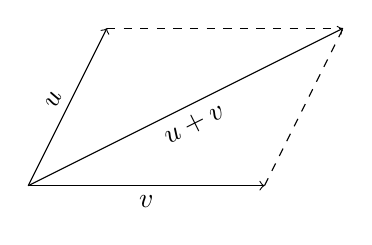
\begin{tikzpicture}
\draw[->] (0,0) -- (1,2) node[midway,sloped,above] {$u$};
\draw[->] (0,0) -- (3,0) node[midway,sloped,below] {$v$};
\draw[dashed] (1,2) -- (4,2);
\draw[dashed] (3,0) -- (4,2);
\draw[->] (0,0) -- (4,2) node[midway,sloped,below] {$u+v$};
\end{tikzpicture} \\
\small{Zasada równoległoboku} \\
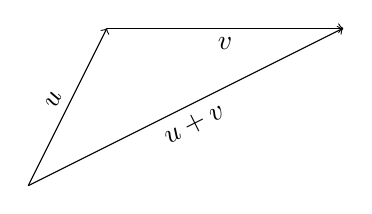
\begin{tikzpicture}
\draw[->] (5,0) -- (6,2) node[midway,sloped,above] {$u$};
\draw[->] (6,2) -- (9,2) node[midway,sloped,below] {$v$};
\draw[->] (5,0) -- (9,2) node[midway,sloped,below] {$u+v$};
\end{tikzpicture} \\ \small{Zasada trójkąta}
\end{minipage}
    
Własności dodawania oraz mnożenia wektorów w $\RR^2 \text{ i } \RR^3$:
\begin{enumerate}[{(}1{)}]
    \item $\forall u, v, w \in \mathbb{R}^2 \quad (u+v)+w = u+(v+w) $
    \item $\forall u, v \in \mathbb{R}^2 \quad u+v = v+u$
    \item $\exists O \in \mathbb{R}^2 \  \forall v \in \mathbb{R}^2 \quad O+v = v+O = v$
    \item $\forall v \in \mathbb{R}^2 \ \exists \text{-} v \in \mathbb{R}^2 \quad v+( \text{-}v) = \text{-} v+v = O$
    \item $\forall u \in \mathbb{R}^2 \ \forall t,s \in \mathbb{R} \quad t(su) = (ts)u$
    \item $\forall u,v \in \mathbb{R}^2 \ \forall t \in \mathbb{R} \quad t(u+v) = tu + tv$ \\ 
          $\forall u \in \mathbb{R}^2 \ \forall t,s  \in
          \mathbb{R} \quad (t+s)u = tu + su$
    \item $\forall u \in \mathbb{R}^2 \quad 1u = u$
\end{enumerate}
    
\begin{ozn} Wektory bazowe będziemy oznaczać jako:
    $e_1 = \begin{pmatrix} 1 \\ 0 \end{pmatrix}$ i $e_2 = \begin{pmatrix} 0 \\ 1\end{pmatrix}$ \end{ozn}
\begin{ft} Każdy wektor w $\RR^2$ zapisuje się jednoznacznie jako kombinacja liniowa wektorów bazowych: $a e_1 + b e_2$ dla pewnych liczb $a$ i $b.$ \end{ft}
    
\begin{df}[algebraiczna]
Iloczynem skalarnym nazywamy funkcję określoną na $\circ\colon\RR^2\times\RR^2\to\RR$ i zadaną wzorem 
\[ \begin{pmatrix} x \\ y\end{pmatrix} \circ \begin{pmatrix} x' \\ y' \end{pmatrix} = xx' + yy' \]
\end{df}
    
Własności iloczynu skalarnego:
\begin{enumerate}[{(}1{)}]
    \item $ \forall u, v \in \RR^2 \ u \circ v = 0 \iff u \perp v$ (przyjmujemy, że wektor $0$ jest prostopadły do każdego wektora)
    \item $ \forall u, v \in \RR^2 \ u \circ v = v \circ u$
    \item $ \forall u, v \in \RR^2 \ \forall t \in \RR \ (tu) \circ v =  t(v \circ u)$
    \item $ \forall u, v, w \in \RR^2 \ u \circ (v + w) = u \circ v + u \circ w$
\end{enumerate}
    
Własności 2, 3, 4 są oczywiste i wynikają wprost z definicji iloczynu skalarnego, natomiast własność 1 najłatwiej jest
pokazać korzystając z definicji geometrycznej iloczynu skalarnego.
    
\begin{df}[geometryczna] 
Iloczyn skalarny można zapisać także w postaci: $$u \circ v = |u||v|\cos\sphericalangle(u, v).$$ \end{df}
    
\begin{tw} Definicja algebraiczna iloczynu skalarnego jest równoważna definicji geometrycznej. \end{tw}
    
\begin{dd}
    Weźmy dowolne dwa wektory $u = ae_1 + be_2$ i $v = a'e_1 + b'e_2$. Łatwo sprawdzić, że obie definicje spełniają
    własności 2, 3 i 4, zatem przekształćmy ich iloczyn skalarny:
    \begin{align*}u \circ v &= (ae_1 + be_2) \circ (a'e_1 + b'e_2) \\
                            &= aa'(e_1 \circ e_1) + ab'(e_1 \circ e_2) + 
                               a'b(e_1 \circ e_2) + bb'(e_2 \circ e_2).
    \end{align*}
    
    Pozostaje pokazać, że zachodzą równości $e_1 \circ e_1 = 1$ oraz $e_1 \circ e_2 = 0$ w obu definicjach. Łatwo. \qed
\end{dd}
    
\begin{tw}[cosinusów]
Niech $a,b,c$ będą długościami boków dowolnego trójkąta i niech $\theta$ będzie kątem naprzeciwko boku o długości $a$, wtedy zachodzi: $c^2 = a^2 + b^2 - 2ab\cos\gamma.$
\end{tw}
    
\begin{dd}
Weźmy dowolne dwa wektory $u,v\in\RR^2$ z kątem $\gamma$ pomiędzy nimi, wtedy wraz z wektorem $w=u-v$ tworzą one trójkąt. Przekształcając: 
\begin{align*} |w|^2 &= w \circ w = (u-v)\circ(u-v) \\ 
                &= u \circ u - u \circ v - v \circ u + v \circ v \\ 
                &= |u|^2 + |v|^2 - 2|u||v|\cos\gamma 
\end{align*}
Kładąc $|u|=a,\ |v|=b, |w|=c$ otrzymujemy tezę. \qed
\end{dd}
    
Analogicznie można zdefiniować powyższe działania i własności dla przestrzeni $\RR^3.$
    
\begin{df}
Wyznacznikiem uporządkowanej pary wektorów $\begin{pmatrix}a \\ b\end{pmatrix}
,\begin{pmatrix} c \\ d \end{pmatrix} $ nazywamy liczbę w postaci: $$\det\begin{pmatrix} a & c \\ b & d\end{pmatrix}=
\begin{vmatrix} a & c \\ b & d \end{vmatrix} = ad - bc.$$
\end{df}
    
Znak wyznacznika informuje nas o orientacji pary wektorów, jeśli jest ujemny, to para wektorów ma orientacje zgodną z
kierunkiem ruchu wskazówek zegara, zaś w przeciwnym przypadku przeciwzegarową.

\begin{center}
    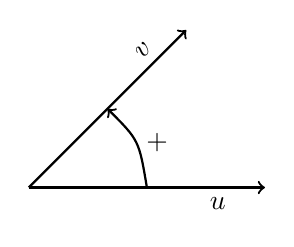
\begin{tikzpicture}
        \draw[thick,->] (0,0) -- (3,0) node[pos=0.8, below] {$u$};
        \draw[thick,->] (0,0) -- (2,2) node[pos=0.8, sloped, above] {$v$};
        \draw[thick,->] (1.5,0) .. controls(1.4, 0.6) ..  (1, 1) node[pos=0.5, right] {$+$};
    \end{tikzpicture}
    \end{center}
\begin{prz}
Para $(u,v)$ jest dodatnio zorientowana.
\end{prz}
    
Wartość bezwzględna wyznacznika równa jest polu równoległoboku rozpinanego przez parę wektorów, skąd możemy otrzymać drugą (równoważną) definicję wyznacznika:

\begin{df}(geometryczna) $\forall u,v\in\RR^2$: $$\det(u,v) = \norm{u}\norm{v}\sin\sphericalangle(u,v).$$ \end{df}
    
\begin{ft}
    Pole dowolnego wielokąta w $\RR^2$ (w którym kolejnie wierzchołki to $v_0,v_1, \dots v_{n-1})$ można wyliczyć za
    pomocą wzoru: 
    \[ \sum_{k=1}^{n-1} \det(v_{k \ mod \ n},v_{k+1 \ mod \ n}) \]
\end{ft}


    
\section{Ciała i przestrzenie liniowe}

\begin{df}
Ciałem nazywamy układ $(K, + ,\cdot,1,0)$, gdzie:
    \begin{itemize}
        \item[] $K$ jest zbiorem
        \item[$+$]: $K \times K \rightarrow K$
        \item[$\cdot$]: $K \times K \rightarrow K$
        \item[] $0 \neq 1 \in K$
    \end{itemize}
    który spełnia następujące warunki (tzw. aksjomaty ciała):
    \begin{itemize}
        \item[(D1)] $\forall a, b, c \in K  \quad (a+b)+c = a+(b+c)$
        \item[(D2)] $\forall a \in K \quad a+0 = 0+a = a$
        \item[(D3)] $\forall a \in K \ \exists \text{-}a \in K \quad a + (\text{-}a) = (\text{-}a) + a = 0$
        \item[(D4)] $\forall a, b \in K \quad a+b = b+a$
        \item[(M1)] $\forall a, b, c \in K \quad (ab)c = a(bc) $
        \item[(M2)] $\forall a \in K \quad 1\cdot a = a\cdot 1 = a$
        \item[(M3)] $\forall a \in K \setminus \{0\} \ \exists a^{-1} \in K \quad a\cdot a^{-1} = a^{-1}\cdot a = 1$
        \item[(M4)] $\forall a, b \in K \quad a\cdot b = b\cdot a$
        \item[(R)] $ \forall a,b, c \in K \quad (a+b)\cdot c = a\cdot c + b\cdot c $
    \end{itemize}
\end{df}

\begin{przy}
    ~\\
    $ \RR, \mathbb{Q}, \mathbb{C} \\
    \mathbb{F}_p = \{0, 1, \dots, p-1\} \text{ gdzie p to l. pierwsza} (+_{mod\ p}, \cdot_{mod\ p})\\
    \mathbb{Q}(\sqrt{2}) = \{a+b\sqrt{2} : a+b \in \mathbb{Q}\}$
\end{przy}

\begin{df}
Przestrzeń liniowa nad ciałem K, to układ $(V,+,\cdot\ ,0)$, gdzie:
\begin{itemize}
        \item[] $V$ jest zbiorem
        \item[+]: $V \times V \rightarrow V$
        \item[$\cdot$]: $K \times V \rightarrow V$
        \item[] $0 \in V$
    \end{itemize}
    który spełnia następujące warunki(tzw. aksjomaty przestrzeni liniowej):
    \begin{itemize}
        \item[(D1)] $\forall u, v, w \in V \quad (u+v)+w = u + (v+w)$
        \item[(D2)] $\forall u \in V \quad u+0 = 0+u = u$
        \item[(D3)] $\forall u \in V \ \exists \text{-}u \in V \quad u + (\text{-}u) = (\text{-}u) + u = 0$
        \item[(D4)] $\forall u, v \in K \quad u+v = v+u$
        \item[(M1)] $\forall a, b \in K\  \forall u \in V \quad (a\cdot b)\cdot u = a\cdot (b\cdot u) $
        \item[(M2)] $\forall u \in V \quad 1\cdot u = u$
        \item[(R1)] $ \forall a,b \in K\ \forall u \in V \quad (a+b)\cdot u = a\cdot u + b\cdot u $
        \item[(R2)] $ \forall a \in K\ \forall u,v \in V \quad a\cdot (u+v) = a\cdot u + a\cdot v $
    \end{itemize}
    \vspace{5mm}
    Elementy przestrzeni liniowej są nazywane wektorami.
    Przestrzeń liniowa czasami jest zwana przestrzenią wektorową.
\end{df}

\begin{przy}
    ~\\
    $\RR^2, \RR^3, \RR^n =
        \left\{
        \begin{pmatrix}
            x_1 \\
            \vdots \\
            x_n
        \end{pmatrix}
        : x_i \in \RR \quad
        \right\}\\
        \ K^n\ (\text{tak samo jak } \RR \text{ tylko } K ) 
        \\
        K[x] \text{ - wielomiany zmiennej x o współczynnikach z } K \\
        K_n[x] \text{ - wielomiany stopnia} \leqslant n \\
        F(\RR,\RR) = \{f: \RR \rightarrow \RR\} \ (f+g)(x) = f(x) + g(x), \ (t\cdot f)(x) = t\cdot f(x),\ t \in \RR \\
        F(\mathbb{N},K) \text{ - zbiór ciągów o wyrazach w } K \\
        C(\RR) = \{f: \RR \rightarrow \RR , f \text{ ciągła} \} \\
        C'(\RR) = \{f: \RR \rightarrow \RR , f' \in C(\RR) \} \\
        C^k(\RR) = \{f: \RR \rightarrow \RR, f^{(k)} \in C(\RR) \} \\
        C^\infty(\RR) = \{f : \RR \rightarrow \RR, f \infty \text{ razy różniczkowalna} \} \ f\text{( to f-kcja gładka)} \\
        \{0\}
    $
\end{przy}

\begin{df}
    Pozdbiór $W \subset V$ przestrzeni liniowej $V$ nazywamy podprzestrzenią (ozn. $W < V$) jeśli jest zamknięta na $+$ i $\cdot$.
\end{df}

\begin{ft}
    Podprzestrzeń $W < V$ też jest przestrzenią liniową (z działaniami obciętymi z działań $V$).
\end{ft}

\begin{dd}
    ~\\
    $ 0\cdot w = 0 \in W$ \\
    $(-1)\cdot w = -w \in W$
\end{dd}
\begin{przy}
    ~\\
    $K_n[x] < K[x]$ \\
    $C^\infty(\RR) < C'(\RR) < C(\RR) < F(\RR,\RR)$ \\
    $\{f \in C(\RR) : \forall x \in [-\infty,0] \ f(x) = 0\} < C(\RR)$ \\
    $\{P \in \RR_4[x] : P(1) = P(2) = 0\} < \RR_4[x]$ \\
    $\{(a_n) \in F(\mathbb{N},\RR) : \forall n \geqslant 2 \quad a_n = a_{n-1} + a_{n-2} \} < F(\mathbb{N},\RR)$ \\
    $\left\{
        \begin{pmatrix}
            x \\
            y \\
            z
        \end{pmatrix}
        \in \RR^3 : 2x + 3y - 4z = 0
        \right\} < \RR^3
    $
\end{przy}
\begin{ft}
    Jeśli $W_i < V $ dla $i \in I$ to $\cap W_i < V$.
\end{ft}

\begin{df}
    Niech $V$ - przestrzeń liniowa nad K. Jeśli $A \subset V$, to \\
    $\operatorname{\Lin}(A) = \cap \{W < V: A \subset W \}$ nazywamy otoczkę liniową $A$ 
    (podprzestrzenią $V$ generowaną przez $A$).
\end{df}
\begin{uw}
    $\Lin(A) < V $ z faktu \thesection.2.
\end{uw}

\begin{przy}
    ~\\
    $\Lin\left\{
        \begin{pmatrix}
            1 \\
            2
        \end{pmatrix}
    \right\} < \RR^2 \text{ (prosta)}
    $ \\
    $\Lin\left\{
        \begin{pmatrix}
            1 \\
            2
        \end{pmatrix},
        \begin{pmatrix}
            0 \\
            1
        \end{pmatrix}
        \right\} < \RR^2 \text{ (cała płaszczyzna)}
    $\\
    $
        \Lin\left\{
        \begin{pmatrix}
            1 \\
            1 \\
            1
        \end{pmatrix},
        \begin{pmatrix}
            1 \\
            0 \\
            3
        \end{pmatrix}
        \right\} < \RR^3 \text{ (płaszczyzna)}
    $ \\
    $
        \Lin\{1,x^2,x^4,\dots\} < R[x] \text{ (wielomiany o parzystych potęgach)}
    $
\end{przy}

\begin{ft}
    $\Lin(A) = \{ \sum\limits_{i=1}^{n} \alpha_i v_i, \quad \alpha_i \in K, v_i \in A\} < V$
\end{ft}

\begin{dd}
    ~\\
    $\subset, \text{ bo } \{ \sum\limits_{i=1}^{n} \alpha_i v_i\} < V$ \\
    $\supset, \Lin(A) < V, \text{więc jest zamknięte na} +,\cdot$
    \qed
\end{dd}
\begin{uw}
    $\Lin(\emptyset)=\{0\} < V $
\end{uw}

\begin{df}
    Zbiór wektorów $ A \subset V $ jest liniowo niezależny (lnz) jeśli żaden z tych wektorów nie jest kombinacją liniową pozostałych.
\end{df}

\begin{prz}
    ~\\
    \begin{minipage}[t]{0.5\textwidth}
    $
    a^{(n)}_i = \begin{cases}
                0 & i \neq n \\
                1 & i = n
              \end{cases}
    $ \\
    $b_i = 1$
    \end{minipage}%
    \begin{minipage}[t]{0.5\textwidth}
       $\overbrace{\{a^{(1)},a^{(2)},\dots,b\}}^{lnz} \subset F(\mathbb{N},\RR)$

    \end{minipage}
\end{prz}

\begin{ft} \hfill
    \begin{enumerate}[{(}1{)}]
         \item $v_1,\dots,v_n$ są liniowo niezależne \\
        $ \hspace*{25mm} \Updownarrow
        \\
        \forall _{\alpha_1,\dots,\alpha_n\in K} (\alpha_1v_1+\dots+\alpha_nv_n = 0 \Rightarrow \alpha_1 = \dots = \alpha_n =0)$
        \item $A \in V $ jest zbiorem lnz $\iff$ każdy skończony podzbiór $A$ jest lnz.
    \end{enumerate}
\end{ft}
\begin{dd} \hfill
    \begin{enumerate}[{(}1{)}]
        \item \begin{itemize}
            \item[($\Downarrow$)] $\alpha_1v_1 + \dots + \alpha_nv_n = 0$ \\
                gdyby $\alpha_i = 0 $, to $v_i$ byłby kombinacją liniową pozostałych \lightning
            \item[($\Uparrow$)] Gdyby nie było lnz, to $v_i = \alpha_1v_1+\dots+ \widehat{\alpha_i v_i} \text{\footnotemark} +\dots + \alpha_nv_n$, to \\ $\alpha_i + \dots + \alpha_{i-1}v_{i-1} - v_i + \dots + \alpha_nv_n = 0 $ \lightning
        \end{itemize}
        \item Każda kombinacja liniowa wykorzystuje skończenie wiele wektorów. \qed
    \end{enumerate}
\end{dd}
\footnotetext{Suma bez elementu pod daszkiem}


\begin{tw}
  Niech $ B \subset V $. Wówczas NWSR:
  \begin{enumerate}[{(}1{)}]
    \item $ B $ jest lnz i $ \Lin(B) = V $
    \item Każdy wektor zapisuje się jednoznacznie jako kombinacja liniowa wektorów z $ B $
    \item $ B $ jest maksymalnym zbiorem lnz
    \item $ B $ jest minimalnym zbiorem generującym
  \end{enumerate}
\end{tw}

\begin{df}
    Bazą $ B $  przestrzeni liniowej $ V $ nazywamy podzbiór spełniający którykolwiek/każdy z równoważnych warunków (1) -- (4).
\end{df}

\begin{dd} \hfill
    \begin{itemize}
        \item[ (3) $\Rightarrow$ (1) ] $ B $ jest maxymalnym zbiorem lnz\\
            Weźmy $ v \in V $. Gdyby $ v \in V \setminus \Lin(B)$, to $ B \cup \{v\}$ byłby lnz. (sprzeczność)
        \item[(1) $\Rightarrow$ (4)] $ B $ jest lnz i generuje $ V $\\
            Gdyby $ B' \subsetneq B$, $ \Lin(B') = V $, to $ v \in B \setminus B'$ byłby kombinacją liniową elementów z $ B'$. (sprzeczność z założeniem $B$ lnz)
        \item[(4) $\Rightarrow$ (2)] $ B $ jest minimalnym zbiorem generującym\\
            Weźmy dowolny wektor $ v \in V $.
            $$ v = \alpha_1v_1 + \dots + \alpha_nv_n = \beta_1v_1 + \dots + \beta_nv_n$$
            gdzie $ \alpha_i, \beta_i \in K, v_i \in B$. Więc
            $$ (\alpha_1 - \beta_1)v_1 + \dots + (\alpha_n - \beta_n)v_n = 0 $$
            Zatem $ \alpha_i = \beta_i $. \\
            (gdyby $ \alpha_i \neq \beta_i $, to $ v_i = -\frac{\alpha_1 - \beta_1}{\alpha_i - \beta_i}v_1 - \dots - \hat{v_i} - \dots -\frac{\alpha_n - \beta_n}{\alpha_i - \beta_i}v_n $,
            czyli $ \Lin(B \setminus \{v_i\}) = V $ co jest sprzeczne z zał. $ B $ - minimalny)
            Więc $ v $ zapisuje się jednoznacznie jako kombinacja liniowa $ B $.
        \item[(2) $\Rightarrow$ (3)] Każdy wektor zapisuje się jednoznacznie jako kombinacja liniowa $ B $\\
            Zauważmy, że $ 0 = 0 v_1 + \dots + 0 v_n $, więc $ \alpha_1 = \alpha_2 = \dots = \alpha_n = 0 $, więc $ B $ jest lnz.
            $ B \cup \{v\} $ nie jest lnz, bo $ v = \alpha_1v_1 + \dots + \alpha_nv_n$. Zatem B jest maksymalnym zbiorem lnz. \qed

    \end{itemize}
\end{dd}


\begin{tw} Każda przestrzeń ma bazę. \end{tw}

\begin{dd}
    ~\\
    $ \{0\} \neq V $ (przestrzeń liniowa) \\
    $ \mathcal{X} = \{ X \subset V : X \text{ lnz} \}, \mathcal{X}  \neq \{0\}$ \\
    Niech $\mathcal{Y} \in \mathcal{X} $ to łańcuch (tzn. $\forall y_1, y_2 \in \mathcal{Y} \ (y_1 \subset y_2 \lor y_1 \supset y_2)$) \\
    $\mathcal{Y}$ ma ograniczenie górne (tzn. $\exists Y \in \mathcal{X} \ \forall y \in \mathcal{Y} \ y \in Y$) \\
    Y $\overset{\mathrm{def}}{=} \bigcup\limits_{y_i \in \mathcal{Y}} y_i \in \mathcal{X}$, bo Y lnz, bo każdy skończony podzbiór Y jest w pewnym $y_i \in $ Y, czyli jest lnz.
    Zgodnie z lematem Kuratowskieg-Zorna w $\mathcal{X}$ istnieje element maksymalny (tzn. max zbiór lnz = baza). \qed
\end{dd}

\begin{prz}
    Istnieje $ B \subset \RR $, taki że każda liczba rzeczywista $ r $ zapisuje się w postaci
    $ q_1r_1 + \dots + q_nr_n $, gdzie $ q_i \in \mathbb{Q}, r_i \in \RR $.
\end{prz}

\begin{tw}
    Niech $ V $ -- przestrzeń liniowa nad $ K $\\
    $ N \subset G \subset V$, gdzie $ N $ lnz, $\Lin(G) = V$\\
    Wówczas istnieje baza $ B $ przestrzeni $ V $, taka że $ N \subset B \subset G $
\end{tw}

\begin{dd}
    $ \mathcal{X} = \{ X \subset V : X \text{ lnz} , N \subset X \subset G\}$ \\
    $ Y = \bigcup y \text{ lnz } V$ \\
    $ N \subset Y \subset G \subset V $ \\
    Zatem z lematu Kuratowskiego-Zorna w $\mathcal{X} $ istnieje element maksymalny  $B \in \mathcal{X}.$
    $B$ lnz. Chcemy $\Lin(B) = V$. Weźmy $g \in G \setminus B.$ Wówczas $N \subset B \cup \{g\} \subset G $ liniowo zależny (lz), czyli $g \in \Lin(B)$. Analogicznie $G \subset \Lin(B)$, czyli $V \subset \Lin(G) \subset \Lin(B)$, czyli B jest bazą. \qed
\end{dd}

\begin{wn} \hfill
    \begin{enumerate}[{(}1{)}]
        \item Każdy zbiór lnz można powiększyć do bazy.
        \item Każdy zbiór generujący zawiera bazę.
    \end{enumerate}
\end{wn}

\begin{tw}
    Każde dwie bazy przestrzeni liniowej $ V $ są równoliczne.
\end{tw}

\begin{df}
    Wymiarem przestrzeni liniowej $ V $ ( $ \dim(V) $ ) nazywamy moc bazy.
\end{df}


%{\color{white} $\widehat{}$} %PROBABLY THE BEST BUG FIX YOU'RE EVER GOING TO FIND
 
    \section{Przekształcenia liniowe} 
\subsection{Homomorfizm}
\begin{df}
    Przekształceniem liniowym (homomorfizmem) przestrzeni liniowych $V \text{ i } W$ nazywamy odwzorowanie $F: V \rightarrow W$ t. że
    \begin{enumerate}[{(}1{)}]
        \item $\forall v, v' \in V \quad F(v+v') = F(v) = F(v')$ (addytywność) 
        \item $\forall v \in V \ \forall \alpha \in K \quad F(\alpha v) = \alpha F(v)$ (jednorodność)
    \end{enumerate}
\end{df}

\begin{przy}
    \hfill
    \begin{enumerate}[{(}1{)}]
        \item $F: \RR^n \rightarrow \RR, \quad F \left( \begin{pmatrix} x_1 \\ \vdots \\ x_n \end{pmatrix}\right) = \alpha_1 x_1 + \dots + \alpha_n x_n \text{, ustalone } \alpha_i \in \RR$ 
        \item $F: \RR^n \rightarrow \RR^m  \quad F \left( \begin{pmatrix} x_1 \\ \vdots \\ x_n \end{pmatrix}\right) = \begin{pmatrix} \alpha_{1,1}x_1 + \dots + \alpha_{1,n} x_n\\ \vdots \\ \alpha_{m,1}x_1 + \dots + \alpha_{m,n} x_n \end{pmatrix}$
        \item $F: K^n \rightarrow K, \quad F \left( \begin{pmatrix} x_1 \\ \vdots \\ x_n \end{pmatrix}\right) = \alpha_1 x_1 + \dots + \alpha_n x_n \text{, ustalone } \alpha_i \in K$ 
        \item $F: K^n \rightarrow K^m  \quad F \left( \begin{pmatrix} x_1 \\ \vdots \\ x_n \end{pmatrix}\right) = \begin{pmatrix} \alpha_{1,1}x_1 + \dots + \alpha_{1,n} x_n\\ \vdots \\ \alpha_{m,1}x_1 + \dots + \alpha_{m,n} x_n \end{pmatrix}$
        \item $F : C'(\RR) \rightarrow C(\RR) \quad F(f) = f'$ 
        \item $F: C(\RR) \rightarrow C(\RR) \quad F(f) = \int\limits_0^x \ f(y) dy$ 
        \item $F: C(\RR) \rightarrow \RR \quad F(f) = \int\limits_a^b \ f(x) dx$ 
        \item $F: \RR [x] \rightarrow \RR[x] \quad F(P)(x) = xP(x)$
        \item $F: C(\RR) \rightarrow \RR \quad F(f) =f(7)$
        \item $L: F(\mathbb{N},\RR)  $ \\ %pierdolona strzałka
        $L((a_1,a_2,\dots)) = (a_2,a_3,a_4,\dots)$ \\
        $R((a_1,a_2,\dots)) = (0,a_1,a_2,\dots)$ 
    \end{enumerate}
\end{przy}
\begin{ft} \hfill 
    \\
    $F: U \rightarrow V $ i $G: V \rightarrow W$ liniowe, to $G \circ F: U \rightarrow W $ liniowe. 
\end{ft}

\begin{dd}
    $(G \circ F)(u+u') = G(F(u+u')) = G(F(u) + F(u')) = G(F(u)) + G(F(u')) = (G \circ F)(u) + (G \circ F)(u') $ (analogicznie jednorodność)
\end{dd}

\begin{df} ~\\
    $F: V \rightarrow W $ p. lin \\
    \underline{Obrazem} F nazywamy \\
    $Im F = \{ F(v): v \in V\}$ \\
    \underline{Jądrem} F nazywamy \\
    $ker(F) = \{v: F(v) = 0\}$
\end{df} 
\begin{ft} \hfill 
    \begin{enumerate}[{(}1{)}]
        \item $Im F < W$
        \item $kerF < V$
    \end{enumerate}
\end{ft}

\begin{dd} 
    $$w,w' \in Im F \quad w=F(v), w'=F(v')$$ 
    $$w+w' = F(v) + F(v') = F(v+v') \Rightarrow w+w' \in ImF $$
    \vspace{5mm}
    $$v,v' \in ker F \quad F(v) = F(v') = 0$$
    $$F(v+v') = F(v) + F(v') = 0 + 0 = 0 \Rightarrow v+v' \in ker F$$ 
    \hfill (podobnie dla mnożenia) \qed
\end{dd}

\begin{uw}
    $F: V \rightarrow W $ liniowe
    $F(0) = F(0_{\in K}\cdot 0_{\in V}) = 0_{\in K} \cdot F(0) = 0_{\in W}$ %AHA
    zatem $\{0\} \subseteq ker F$.
\end{uw}

\begin{ft} 
    ~\\
    $F: V \rightarrow W $ p. lin jest różnowartościowe \\
    $ \hspace*{30mm} \Updownarrow \\
        \hspace*{20mm} ker F = \{ 0 \}
    $
\end{ft}

\begin{dd} \hfill
    \begin{itemize}
        \item[$(\Uparrow)$] $F(v) = F(v') \\ 
            F(v)-F(v') = 0 \\
            F(v-v') = 0 \\
            ker F \ni v-v' = 0 \\
            v = v' 
        $ \qed
        \item[$(\Downarrow)$] oczywiste
    \end{itemize}
\end{dd}

\begin{tw}[o indeksie]
    ~\\
    $F: V \rightarrow W $ liniowe, to $dimker F + dimIm F = dim V$
\end{tw}
\begin{dd}
    $ker F < V,\  Im F < W$ \\
    \begin{minipage}[c]{0.5\textwidth}
        $B$ - bzaza $ker F$ \\
        $ B \cup B' $ - baza $V$
    \end{minipage}%
    \begin{minipage}[c]{0.5\textwidth}
        $B = \{b_i\}_{i \in I}$ \\
        $B' = \{b'_i\}_{i \in J}$ \\
        $I \cap J = \emptyset $
    \end{minipage} \\
    bazą $Im F$ jest $\{F(b'_i)\}_{i \in J}$ \\
    Będziemy teraz udowadniać, że to rzeczywiście jest baza\\
    $w \in Im F$ \\
	%\includegraphics[width=5cm]{wyklad3_obrazek} \\ % konwertowanie:
    %%%
    $w = F(v) = F(\sum\limits_{i \in I'} \alpha_i b_i + \sum\limits_{i \in J'} \alpha'_i b'_i) = \sum\alpha_i b_i + \sum\alpha'_i b'_i = \sum\alpha'_i b'_i $\\
    $(|I'|, |J'|<\infty \quad I'\subset I, J'\subset J)$\\
    więc $\{F(b'_i)\}_{i \in J} $ generuje $ImF$ \\
    lnz: \\
    $\sum\limits_{i\in J} \alpha'_i F(b_i') = 0$\\
    $\qquad \rotatebox{90}{$\,=$}$\\%nie umiem zrobić odstępu :(
    $F(\sum \alpha'_i b_i') \quad $więc $ \sum \alpha'_i b_i' \in imF$\\
    $\sum \alpha'_i b_i' =\alpha_i b_i$ \quad kombinacja liniowa bazy $kerF$\\
    $B\cup B'$ jest bazą V więc $\alpha_i' = \alpha_i = 0$ \quad \qed
     % dopisać resztę linijki 
    %wniosek generuj Im i dowód lnz
\end{dd} 

\begin{prz}
    $ V = \{ P \in \RR_4[x] : P'(0) + P(0) = P(1) = 0 \}$ 
    \begin{itemize}
        \item V jest p. liniową
        \item Obliczyć $dim V$
    \end{itemize}
    $ F : \RR_4[x] \rightarrow \RR^4 
        \qquad F(P) = \begin{pmatrix} P'(0) + P(0) \\ P(1) \end{pmatrix} $ \quad $F$ jest liniowe \\
    $V = ker F$, czyli $V < \RR_4[x]$
    $dim V = dimker F = dim\RR_4 [x] = dimImF$ %skrabione znaki równa się \\
    $F(1) = \begin{pmatrix} 1 \\ 1 \end{pmatrix} \in Im F$ \\
    $F(x^2) = \begin{pmatrix} 0 \\ 1 \end{pmatrix} \in Im F$
    $Lin \left\{ \begin{pmatrix} 0 \\ 1 \end{pmatrix} \begin{pmatrix} 1 \\ 1 \end{pmatrix} \right\} < Im F < \RR^2 $, czyli
    $Im F = \RR^2$ \\%+ popierdolone równa się xD
    $dimV = dim\RR[x] - dimImF = 5 - 2 = 3$
\end{prz}

\begin{df} 
    Przekształcenie liniowe $F: V \rightarrow W $ nazywamy odwracalnym $\Leftrightarrow$ istnieje $G: W \rightarrow V$ liniowe t. że $F \circ G - id_W, G \circ F = id_V.$ Przekształcenie odwrotne (o ile istnieje) jest jedyne i oznaczamy je $F^{-1}$. \footnote{$(F \circ G)(v) = F(G(v))$}
\end{df}

\begin{ft} $F: V \rightarrow W $, liniowe, $dim V = dimW < \infty$. Wówczas NWSR:
    \begin{enumerate}[{(}1{)}]
        \item $F$ różnowartościowe (tzn. $kerF = \{0\}$)
        \item $F$ jest "na" (tzn. $Im F = W$)
        \item $F$ jest bijekcją
    \end{enumerate}
\end{ft}

\begin{dd} 
    ~\\
    $dimker F + dimIm F = dim V = dim W$
    \begin{itemize}
        \item[$(1) \Rightarrow (2)$] $
            dimker F = 0, \qquad Im F < W \\
            dimIm F = dim W \\ 
            Im F = W$
        \item[$(2) \Rightarrow (3)$]
            $
            dimImF = dimW \\
            dimkerF = 0 \\ 
            kerF = \{0\} \\
            F
            $ różnowartościowa + "na"
        \item[$(3) \Rightarrow (1)$] oczywiste
    \end{itemize} 
\end{dd}
\subsection{Macierze}
\begin{df} 
    Niech $B = (b_1,\dots,b_n) $ będzie bazą przestrzeni liniowej V. Wówczas \underline{współrzędnymi} wektora $v \in V$ w bazie B nazywamy: 
        $$ [v]_B = \begin{pmatrix} \alpha_1 \\ \vdots \\ \alpha_n \end{pmatrix} \quad \alpha_i \in K$$ \\
        gdzie $ v = \alpha_1 b_1 + \dots + \alpha_n b_n$.
\end{df}
\begin{df} 
    $ 
        F: V \rightarrow W \text{p. liniowa nad K} \\
        B = (b_1,\dots,b_n) \text{ - baza V},
        C = (c_1, \dots,c_m) \text{ - baza W} \\
    $
    Wówczas macierz 
    \[m^B_C (F) = ([F(b_1)]_C,\dots,[F(b_n)]_C)\] 
    nazywamy \underline{macierzą przekształceń $F$} w bazach $B$ i $C$. 
    \[ A = \begin{pmatrix} a_{11} \ a_{12} \ \dots \ a_{1n} \\
                           a_{21} \ a_{22} \ \dots \ a_{2n} \\
                                   \        \vdots \  \\
                           a_{m1} \ a_{m2} \ \dots \ a_{mn}
               \end{pmatrix} \quad A \in M_{m \times n} (K) \]
    %~\\
\end{df}
\underline{Dodawanie macierzy} \\
$ 
  A = (a_{ij}) \\
  A' =(a'_{ij}) \\ 
  B = A + A' = (b_{ij}), \text{gdzie} b_{ij} = a_{ij} + a'_{ij}
$ \\
\underline{Mnożenie macierzy przez skalar} \\ 
$ 
    t \in K, (a_{ij}) = A \in M_{m \times n}(K) \\
    tA = B = (b_{ij}) \quad b_{ij} \overset{\mathrm{def}}{=} t a_{ij}
$ \\
\underline{Mnożenie macierzy} \\ 
$
    A = (a_{ij}) \in M_{m \times n} \\
    B = (b_{ij}) \in M_{n \times l} \\ 
    C = A \cdot B = (c_{ij}) \in M_{m \times l} \\
    c_{ij} \overset{\mathrm{def}}{=} \sum\limits_{k=1}^n a_{ik}b_{kj}
$
\begin{ft}
    Mnożenie \\
    $A', A \in M_{k \times l} (K) \hspace{0.5cm} B', B \in M_{l \times m} (K) \hspace{0.5cm} C \in M_{m \times n} (K)$
    \begin{enumerate}[{(}1{)}]
        \item $ (A \cdot B) \cdot C = A \cdot (B \cdot C)$
        \item $ (A + A') \cdot B = A \cdot B + A' \cdot B \\
            A \cdot (B + B') = A \cdot B + A \cdot B' $
        \item $ I_k \cdot A = A  \cdot I_l = A  \hspace{1cm} \text{gdzie } I_k = \begin{pmatrix} 
                1 & & 0 \\ & \ddots & \\ 0 & & 1
            \end{pmatrix} $
    \end{enumerate}
\end{ft}

\begin{ft}
    Niech \\ $ F: V \rightarrow W $ będzie przekształeceniem liniowym.\\
    $ B = (b_1, \ldots , b_n) \text{ - bazą } V \\
      C = (c_1, \ldots , c_n) \text{ - bazą } W $ \\
    Wówczas:
    $$ [F(v)]_C = m^B_C(F) \cdot [v]_B \text{ ,gdzie } v \in V$$
\end{ft}

\begin{wn}
    $ id: V \rightarrow V,\quad B, C \text{ - bazy } V$
    $$ [v]_c = m^B_C(id) \cdot [v]_B $$
    gdzie $ m^B_C(id) = ( [b_1]_C, \ldots , [b_n]_C)$
\end{wn}

\begin{ft}
    Niech \\ $ F: U \rightarrow V, G: V \rightarrow W $ będą przekształceniami liniowymi.\\
  $ B \text{ - bazą } U\\
    C \text{ - bazą } V\\
    D \text{ - bazą } W\\ $
Wtedy: $m^B_D(G \circ F) = m^C_D(G) m^B_C(F)$
\end{ft}
\begin{wn}
$ id: V \rightarrow V,\quad B, C \text{ - bazy } V$
    Wtedy: $$ m^B_B(F) = m^C_B(id) \cdot m^C_C(F) \cdot m^B_C(id)$$

\begin{tw} 
    ~\\
    $ F: V \rightarrow W \text{ p. liniowe}$ \\
    baza $V$ --- $B=(b_1, ..., b_n)$ \\
    baza $W$ --- $C=(c_1, ..., c_n)$ 
    $$ [F(v) ]_C = m^B_C(F)[v]_B $$ 
    gdzie $m^B_C(F)=([F(b_1)]_C, ..., [F(b_n)]_C)$.
\end{tw}

\begin{dd}
    Weźmy $v \in V$ i~jego przedstawienie $v=\sum\limits_{i=1}^n\alpha_ib_i = [v]_B$.
    \[F(v)=F\left(\sum_{i=1}^n\alpha_ib_i\right)=\sum_{i=1}^n\alpha_iF(b_i)\]
    \[F(b_i)=\sum_{j=1}^m\beta_{ji}c_j\]
    gdzie
    \[\begin{pmatrix}\beta_{1i} \\ \vdots \\ \beta_{mi}\end{pmatrix}=[F(b_i)]_C\]
    \[F(v)=\sum_{i=1}^n\alpha_iF(b_i)=\sum_{i=1}^n\alpha_i\sum_{j=1}^m\beta_{ji}c_j=\]
    \[=\sum_{i=1}^n\sum_{j=1}^m(\alpha_i\beta_{ji})c_j=\sum_{j=1}^m\left(\sum_{i=1}^n\alpha_i\beta_{ji}\right)c_j\]
    \[[F(v)]_C=\begin{pmatrix}\sum\limits_{i=1}^n\beta_{1i}\alpha_i\\ \vdots \\\sum\limits_{i=1}^n\beta_{mi}\alpha_i\end{pmatrix}=
     \begin{pmatrix}\beta_{11}& \dots &\beta_{1n}\\ \vdots & \vdots & \vdots\\\beta_{m1}& \dots&\beta_{mn}\end{pmatrix}
    \begin{pmatrix}\alpha_1\\ \vdots \\\alpha_n\end{pmatrix}  \] \hfill \qed
\end{dd}

\begin{wn}
    \[ B = (b_1, ..., b_n) \]
    \[ C = (c_1, ..., c_n) \]
    obie są bazami $V$, więc
    \[ [V]_C = m^B_C(id)[v]_B \]
    gdzie $m^B_C(id)=([b_1]_C, ..., [b_n]_C)$
    
    Jest to macierz przekształcenia.
    Baza standardowa $\varepsilon=(e_1, ..., e_n)$ występuje
    w~przestrzeniach $K^n$, gdzie
    \[e_i=\begin{pmatrix}0 \\ \vdots \\ 0 \\ 1 \\ 0 \\ \vdots \\ 0\end{pmatrix} \leftarrow i\]
\end{wn}

\begin{tw}
    \[ F: V \rightarrow W \mathrm{p. liniowe} \]
    \[ G: U \rightarrow V \mathrm{p. liniowe} \]
    baza $U$ --- $B=(b_1, ..., b_k)$ \\
    baza $V$ --- $C=(c_1, ..., c_l)$ \\
    baza $W$ --- $D=(d_1, ..., d_m)$ 
    \[m^B_D(F\circ G)=m^C_D(F)m^B_C(G)\]
\end{tw}

\begin{dd} 
    ~\\
    $U \overset{G}{\longrightarrow}  V \overset{F}{\longrightarrow} W$ \\ 
    $[(F\circ G)(u)]_D = m_D^B(F\circ G)[u]_B$ \\
    $[F(G(u))]_D = m_D^C(F) \cdot [G(u)]_C = m_D^C \cdot (m_C^B(G)[v]_B)$
\end{dd}

\begin{wn} \hfill
    \begin{itemize}
        \item $K^k \overset{G}{\longrightarrow} K^l \overset{F}{\longrightarrow} K^m $\\
              $ F(X) = AX, \qquad G(X) = BX $ \\ 
              $(F\circ G)(X) = F(G(X)) = A(BX) = (AB)X$
        \item $ F: V \rightarrow W \mathrm{ p.liniowe} $ \\
              $ F^{-1}: W \rightarrow V \mathrm{ p. liniowe} $ \\
              baza $V$ --- $B=(b_1, ..., b_n)$ \\
              baza $W$ --- $C=(c_1, ..., c_n)$ \\
              $m^B_C(F)m^C_B(F^{-1}) = I $ \\
              $m^C_B(F^{-1})m^B_C(F) = I $
    \end{itemize}
\end{wn}


\end{wn}

    \section{Izomorfizmy}
\begin{df}
    Przekształcenie liniowe $F: V \rightarrow W$ nazywamy
    \textbf{izomorfizmem}, jeśli istnieje przekształcenie
    liniowe $G: W\rightarrow V$, takie że $G\circ F = id_V$
    i~$F\circ G=id_W$.
\end{df}

\begin{ft}
    $F: V \rightarrow W$ jest izomorfizmem $\Leftrightarrow$ jest liniową
  bijekcją.
\end{ft}

\begin{dd} ~\\
    $\Rightarrow$ oczywiste\\
  $\Leftarrow$ $F^{-1}: W \rightarrow V$ (funkcja)
  Potrzeba pokazać, że $F^{-1}$ jest liniowa. Przykładowo:
  $$F^{-1}(w+w')=F^{-1}(F(v)+F(v'))=F^{-1}(F(v+v'))=v+v'=F^{-1}(w)+F^{-1}(w')$$ 
  Analogicznie dowodzimy jednorodność.
\end{dd}

\begin{df}
    Przestrzenie liniowe $V$ i~$W$ są izomorficzne ($V \simeq W$), gdy istnieje
    izomorfizm $F: V \rightarrow W$.
\end{df}

\begin{przy}
    \[K^n \simeq K_{n-1}[x]\]
    \[F: K^n \rightarrow K_{n-1}[x]\]
    \[\begin{pmatrix}a_0\\ \vdots \\a_n\end{pmatrix} \overset{F}{\longmapsto}
    \left(a_0+a_1x+...+a_{n-1}x^{n-1}\right)\]
    
    $F$ --- bijekcja, liniowa.
    
    \vspace{5mm}
    $M_{m\times n}(K)$ --- przestrzeń liniowa nad $K$.
  \[M_{m\times n}(K) \simeq K^{mn}\]
  \[F: M_{m\times n}(K) \rightarrow K^{mn}\]

  \[(a_{ij}) \longmapsto \begin{pmatrix}a_{11}\\ \vdots\\a_{1n}\\
    a_{21}\\ \vdots \\a_{mn}\end{pmatrix}\]
\end{przy}

\begin{tw}
    Jeśli $V$ jest skończenie wymiarową przestrzenią liniową nad $K$, to
  \[V \simeq K^n\]
  gdzie $n=\dim V$.
\end{tw}

\begin{dd}
    Niech $B=(b_1, ..., b_n)$ będzie bazą $V$. Wówczas
  \[F: V \rightarrow K^n\]
  \[F(v) = [v]_B\]
  jest izomorfizmem.
\end{dd}

\section{Macierz odwrotna}

\begin{df}
    \textbf{Macierzą odwrotną} do $A \in M_{n\times n}(K)$ nazywamy macierz
  $B \in M_{n\times n}(K)$ taką, że
  \[AB = BA = I\]
\end{df}

\begin{ft}
    Dla $A,B \in M_{n\times n}(K)$ zachodzi
    \[AB=I \Rightarrow BA=I\]
\end{ft}

\begin{df}
    Operacjami elementarnymi (wierszowymi) na macierzy prostokątnej $A$
    nazywamy następujące operacje:
    \begin{enumerate}[{(}1{)}]
        \item zamiana miejscami $i$-tego i~$j$-tego wiersza ($i \neq j$)
        \item przemnożenie $i$-tego wiersza przez $\alpha \in K \setminus \{0\}$
        \item dodanie do $j$-tego wiersza $\alpha$-krotności $i$-tego wiersza
          ($i \neq j$, $\alpha \in K \setminus \{0\}$)
    \end{enumerate}
    Analogicznie definiujemy operacje elementarne (kolumnowe).
\end{df}

\begin{uw}
    Wszystkie te operacje można zapisać mnożąc z~lewej (wierszowe) lub
  z~prawej (kolumnowe) przez odpowiednią macierz.

  Ad 1. (zamiana $i$ i $j$)
  \[\begin{pmatrix}
     1 &...&...&...\\
    ...& 0 & 1 &...\\
    ...& 1 & 0 &...\\
    ...&...&...& 1
  \end{pmatrix}\begin{pmatrix}
    a_{11}&...&a_{1n}\\
    ...&a_{jk}&...\\
    ...&a_{ik}&...\\
    a_{m1}&...&a_{mn}
  \end{pmatrix}=\begin{pmatrix}
    a_{11}&...&a_{1n}\\
    ...&a_{ik}&...\\
    ...&a_{jk}&...\\
    a_{m1}&...&a_{mn}
  \end{pmatrix}\]

  Analogicznie, wykonanie elementarnej operacji na $A$ to
  mnożenie $A$ przez pewną macierz $B_{op}$.
  
  $B_{op}$ to po prostu $I$, na ktorym została wykonana ta operacja.
\end{uw}

\begin{ft}
    \[A = (a_{ij}) \in M_{m\times n}(K)\]
  \begin{enumerate}
    \item Jeśli ciąg operacji elementarnych \textit{wierszowych} przeprowadza
      macierz \[(A|I)=\begin{pmatrix}
        a_{11}&...&a_{1n}& 1 &...& 0 \\
        ...&...&...&...& 1 &...\\
        a_{m1}&...&a_{mn}& 0 &...& 1 \\
      \end{pmatrix}\]
      na $(I|B)$, to $B = A^{-1}$
    \item Albo istnieje ciąg operacji elementarnych wierszowych
      przeprowadzających $A$ na~$I$, albo istnieje ciąg operacji
      wierszowych zamieniających $A$ na~macierz z~zerową kolumną /
      zerowym wierszem
  \end{enumerate}
\end{ft}

\begin{dd}
    \[(E_k...E_2E_1)A=I\]
  \[E_k...E_2E_1I=E_k...E_2E_1=A^{-1}\]
\end{dd}

\section{Wyznacznik}
    Intuicyjnie: $n$-wymiarowa objętość (dim = 1: długość, dim = 2: pole powierzchni, dim = 3: objętość). \\
    Zerowy wyznacznik oznacza liniową zależność wektorów w~macierzy. \\
    Wzory Kramera --- rozwiązywanie układów równań przy pomocy wyznaczników.

\begin{df}
    Odwzorowanie
  $F: \underbrace{V \times V \times ... \times V}_{n} \rightarrow K$
  (gdzie $V$ jest przestrzenią liniową nad $K^n$) nazywamy:
  \begin{enumerate}
    \item \textbf{wieloliniowym}, jeśli
      $\forall_k\forall_{v_i,v_{i'}\in V}\forall_{\alpha\in K}$:
      \[F(v_1, ..., v_k+v_{k'}, ..., v_n)
      = F(v_1, ..., v_k, ..., v_n) + F(v_1, ...,v_{k'}, ..., v_n)\]
      oraz
      \[F(v_1, ..., \alpha v_k, ..., v_n) = \alpha F(v_1, ..., v_n)\]
    \item \textbf{antysymetrycznym}, jeśli $\forall_{i,j}$:
      \[F(v_1, ..., v_i, ..., v_j, ..., v_n)
      = -F(v_1, ..., v_j, ..., v_i, ..., v_n)\]
  \end{enumerate}
\end{df}

\begin{tw}
    Dla każdej liczby $c \in K$ istnieje dokładnie jedno odwzorowanie
    \[F: \underbrace{K^n \times K^n \times ... \times K^n}_{n} \rightarrow K\]
    które jest $n$-liniowe, antysymetryczne oraz $F(I) = c$.
\end{tw}

\begin{dd}
    \[e_i=\begin{pmatrix}0\\ \vdots \\1\\ \vdots \\0\end{pmatrix} \leftarrow i\]
  \[A=(a_{ij})=(A_1, ..., A_n)\]
  \[F(A_1, ..., A_n) = F(\sum_{i_1}a_{i_1}e_{i_1}, ..., \sum_{i_n}a_{i_n}e_{i_n}) =\]
  (z~$n$-liniowości)
  \[= \sum_{i_1}...\sum_{i_n}a_{i_1}...a_{i_n}F(e_{i_1}, ..., e_{i_n}) =\]
  (z~antysymetryczności) $F(...v...v...)=-F(...v...v...)$,
  czyli $2F(...v...v...)=0$. Dla ciał, że $1+1=0$ też, z~inną def. antysymetryczności)
  \[= \sum_{\sigma\in S_n}a_{\sigma(1)1}...a_{\sigma(n)n}F(e_{\sigma(1)}, ..., e_{\sigma(n)}) = \]
  \[= \sum_{\sigma\in S_n} \pm a_{\sigma(1)1}...a_{\sigma(n)n}F(e_1, ..., e_n)\]
  gdzie $F(e_1, ..., e_n)=c$.
  \[\sigma: \{1, 2, ..., n\} \overset{\mathrm{na}}{\underset{\mathrm{,,1-1''}}{\longrightarrow}} \{1, 2, ..., n\}\]

\end{dd}

\begin{lem}
    Jeśli permutację $\sigma$ rozłożymy na złożenie transpozycji, to $(-1)^{\#\mathrm{transpozycji}}$ jest niezależna od rozkładu (i~oznaczana jest $\mathrm{sgn}(\sigma)$).
\end{lem}

\begin{dd}
    Zdefiniujmy $t(\sigma)$ jako:
  \[t(\sigma)=\{(i,j): i<j \land \sigma(i)>\sigma(j)\}\]
  liczbę nieporządków\\
  Przykład:
  \[\begin{pmatrix}1&...&n\\\sigma(1)&...&\sigma(n)\end{pmatrix}
    =\begin{pmatrix}1&2&3&4&5\\5&4&1&3&2\end{pmatrix}\]

  \[t(\sigma) = 8\]
  \[\mathrm{sgn}(\sigma) = (-1)^8 = +1\]
  \[\sigma(id) = 0\]

  Transpozycja to permutacja postaci:
  \[\begin{pmatrix}
    1&...&i&...&j&...&n\\
    1&...&j&...&i&...&n
  \end{pmatrix}\]

  \[t(\mathrm{transpozycja})=2(j-i-1)+1\]
  a~zatem
  \[\mathrm{sgn}(\mathrm{transpozycja})=-1\]

  Wystarczy pokazać, że jeśli
  \[\sigma' = \tau \circ \sigma\;,\qquad \tau=\mathrm{transpozycja}\]
  to
  \[t(\sigma') \equiv t(\sigma)+1 \;(\mathrm{mod}\; 2)\]
  \[1^\circ\; \sigma(i) < \sigma(j)\]
  \[2^\circ\; \sigma(i) > \sigma(j)\]
  czyli \#transpozycji $\equiv t(\sigma)$ (mod 2).
  zatem $(-1)^{\#\mathrm{transpozycji}}$ nie zależy od rozkładu.\\
  Pozostaje sprawdzić, że otrzymany wzór
  \[F(A_1, ..., A_n)=\sum_{\sigma \in S_n}\mathrm{sgn}(\sigma)a_{\sigma(1)1}...a_{\sigma(n)n}\]
  spełnia zadane warunki. \qed
\end{dd}

\begin{df}
    Wyznacznikiem nazywamy \textit{jedyną} funkcję
  \[\det: (K^n)^n \rightarrow K\]
  \[\left((K^n)^n \simeq M_{n \times n}(K)\right)\]
  która jest $n$-liniowa, antysymetryczna i~$\det I=1$
\end{df}

\begin{ft}
    \[\det A^T = \det A\]
  \[\begin{vmatrix}1&2&3\\1&4&1\\2&0&0\end{vmatrix}
    =\begin{vmatrix}1&1&2\\2&4&0\\3&1&0\end{vmatrix}\]
\end{ft}
\begin{dd}
    \[\sum_\sigma\mathrm{sgn}(\sigma)a_{\sigma(1)1}...a_{\sigma(n)n}\]
    \[\sum_\sigma\mathrm{sgn}(\sigma^{-1})a_{\sigma^{-1}(1)1}...a_{\sigma^{-1}(n)n}\]
    \[\sum_{\sigma^{-1}}\mathrm{sgn}(\sigma^{-1})a_{\sigma^{-1}(1)1}...a_{\sigma^{-1}(n)n}\]
\end{dd}

\begin{wn}
    Dla macierzy $A \in M_{n \times n}(K)$ wyznacznik $\det A$:
    \begin{enumerate}[{(}1{)}]
        \item zmienia znak przy zamianie miejscami dwóch wierszy/kolumn
        \item nie zmienia się po dodaniu krotności jednego wiersza/kolumny do innego
        \item mnoży się przez $t \in K$ przy pomnożeniu przez $t$ wybranego
          wiersza/kolumny
    \end{enumerate}
\end{wn}

\begin{dd} \hfill
    \begin{enumerate}[{(}1{)}]
        \item Antysymetryczność
        \item $\det(A_1,\dots,A_i+tA_j,\dots,A_n) = \det(A_1,\dots,A_i,\dots,A_n) + \\ + t \overbrace{\det(A_1,\dots,A_i,\dots,A_i
        ,\dots,A_n)}^0 = \det(A_1,\dots,A_n)$
        \item $\det(A_1,\dots,tA_i,\dots,A_n) = t \det(A_1,\dots,A_i,\dots,A_n)$
    \end{enumerate}
\end{dd}

\begin{tw}[o rozwinięciu Laplace'a] ~\\
    Dla $A \in M_{n \times n} (K) $ oraz ustalonego $i \in \{1,\dots,n\}$ 
        $$\det(A) = \sum_{j=1}^n (-1)^{i+j} a_{ij} A_{ij}$$
        gdzie $A_{ij}$ to wyznacznik macierzy A z usuniętym i-tym wierszem i j-tą kolumną. 
        \end{tw}
\begin{uw}
    Twierdzenie jest prawdziwe gdy zamienimy miejscami i i j.
\end{uw}

\begin{dd} 
    $\det A^T = \det A$, więc wystarczy pokazać dla wierszy. \\
    \textit{intuicja}: Liczenie wyznacznika to liczenie rozstawień wież na szachownicy, tak aby się wzajemnie nie szachowały. Patrząc na wzór widać, że jest to dokładnie to w postaci rekurencyjnej. Jedyne, co zostało sprawdzić to czy znak się zgadza.
    $$\sigma : \{1,\dots,n\} \rightarrow \{1,\dots,n\} $$ 
    $$\sigma (i) = j$$
    $$\sigma_{ij} = \{1,\dots,\hat i, \dots, n\} \rightarrow \{1,\dots,\hat j, \dots, n\} $$
    $$ \{1,\dots,n-1\} \qquad \{1,\dots,n-1\} $$
    $$ sgn(\sigma) \overset{?}{=} (-1)^{i+j} sgn(\sigma_{ij})$$
    $$ n(\sigma) = n(\sigma_{ij}) + \underbrace{|\{k < i: \sigma(k)  > j\}|}_x + |\{k > i : \sigma(k) < j\}| \footnote{chodzi o nieporzadki}$$ 
    $$ n(\sigma) = n(\sigma_{ij} + 2x + j - i $$
    $$ n(\sigma) = n(\sigma_{ij}) + (i+j) + 2(x - i) $$
    $$ n(\sigma) = n(\sigma_{ij} + (i+j) mod 2 $$
    $$ (-1)^{n(\sigma)} = (-1)^{n(\sigma_{ij})} (-1)^{i+j}$$
    $$ sgn(\sigma) = sgn(\sigma_{ij}) \cdot (-1)^{i+j} $$
    \hfill \qed
\end{dd}

    \subsection{Zastosowanie wyznaczików macierzy}
\begin{tw} 
     $$
     (\ast) \left\{ 
        \begin{array}{l}
        a_{11} x_{1} + \dots a_{1n} x_{n} = b_1 \\
        \vdots \\
        a_{n1} x_{1} + \dots a_{nn} x_{n} = b_n 
        \end{array}
    \right.$$
    $$
    \text{inaczej}
    \begin{pmatrix} 
        a_{11} \ \dots \ a_{1n} \\
         \ \vdots \ \\ 
        a_{n1} \ \dots \ a_{nn} 
    \end{pmatrix}
    \begin{pmatrix}
        x_1 \\ 
        \vdots \\ 
        x_n
    \end{pmatrix}
    = 
    \begin{pmatrix}
        b_1 \\ 
        \vdots \\ 
        b_n
    \end{pmatrix} 
    \text{lub jeszcze inaczej } A\footnote{macierz A to macierz główna układu}X = b
    $$
    Układ $(\ast)$ ma jednoznacznie rozwiązanie $\Leftrightarrow$ $\det A \neq 0 $ i rozwiązanie ma postać 
    $x_i = \frac{\det A^{(i)}}{\det A}$, gdzie $A^{(i)} = (A_1,\dots,\overset{i}{b},\dots,A_n)$
\end{tw}

\begin{dd} 
    $$ A  \overset{ozn}{=} (A_1,\dots,A_n) $$ 
    $$(\ast) x_1A_1 + x_2A_2 + \dots + x_nA_n = b$$
    $$ \det A^(i) = det(A_1,\dots,\underset{i}{b},\dots,A_n) = \det(A_1,\dots,A_{i-1},\sum_{k=1}^n x_kA_k,A_{i+1},\dots,A_n) = $$
    $$ = \sum_{k=1}^n x_k \det(A_1,\dots,A_{i-1},A_k,A_{i+1},\dots,A_n) = x_i \det (A_1,\dots, A_{i-1},A_i,A_{i+1},\dots,A_n) = $$
    $$ = x_i = \det A$$
    $$ \det A^{(i)} = x_i \det A$$
Jeśli $det A \neq 0$ to $x_i = \frac{\det A^{(i)}}{\det A}$. \\
Jeśli $\det A = 0$, to $ker F \neq \{0\}, F: K^n \rightarrow K^n : F(X) = AX$

\begin{lem}
    Odwozrowanie $F: K^n \rightarrow K^n \text{t. że} F(X) = AX $ jest różnowartościowe/na/odwaracalne/ bijekcją ma trywialne jądro.$\Leftrightarrow \det A \neq 0$
\end{lem}
$ F^{-1} [b] = 
    \begin{cases} 
        \emptyset & \text{jeśli } b \notin \operatorname{Im} F\\ 
        \{v\} + \ker F & \text{jeśli } b \in \operatorname{Im} F,\text{ dla pewnego } v \in V
    \end{cases}$ \\
$ \dim ker F > 0 \Rightarrow \dim ImF < n \Rightarrow ImF \neq K^n $ \\
$b = F(v)$ dla pewnego $v \in V$ \\ 
$ \underset{w \in ker F}{F(v+w)} = F(v) + \underscript{F(w)}{\verteq}{0} = F(v) = b$ 
\begin{align}
    b &= F(v) \label{jeden}\\
    b &= F(v') \label{dwa} \\
    \shortintertext{Odejmując \eqref{jeden} od \eqref{dwa} otrzymujemy}
    0 &= F(v) - F(v') = F(v-v'), \text{ czyli } v-v' \in ker F \notag
\end{align}
    $v = v' + \underscript{(v - v')}{\vertin}{\ker F}$
\end{dd}

\begin{dd}
  (lematu)

  Jeśli $F$ jest odwracalna, to istnieje $G: K^n \rightarrow K^n$, $G(X)=BX$,
  takie że
  \[F \circ G = G \circ F = id\]
  \[m(F \circ G) = m(G \circ F) = I\]
  \[AB = BA = I\]
  czyli $B=A^{-1}$ ($A$ odwracalna).
  \[1 = \det (AB) \overset{\text{ćw}} = \det A \det B\]
  więc $\det A \neq 0$.

  W~drugą stronę ($\det A \neq 0 \Rightarrow A \text{ odwracalna} \land B \text{ odwracalna}$) to wniosek z~następnego faktu.
  \hfill \qed
\end{dd}
\begin{ft}
  $B = (b, j)$ jest macierzą odwrotną do $A$, wtedy i~tylko wtedy, gdy:
  \[b_{ji} = \frac1{\det A}(-1)^{i+j} +
  \begin{vmatrix}
  & & & \\ 
  & a_{ij} \makebox(-10,0){\rule[4mm]{0.4pt}{2.5\normalbaselineskip}} 
      \makebox(-10,0){\rule[2.5mm]{2.5\normalbaselineskip}{0.4pt}} 
  & \\ 
  & & &
  \end{vmatrix}
  \]
\end{ft}
\begin{prz}
  \[A = \begin{pmatrix}1&0&1\\0&2&1\\1&1&1\end{pmatrix}\qquad\det A = -1\]
  \[A^{-1}=\frac1{-1}\begin{pmatrix}1&+1&-2\\+1&0&-1\\-2&-1&2\end{pmatrix}^T
    =\begin{pmatrix}-1&-1&2\\-1&0&-1\\2&1&-2\end{pmatrix}\]
\end{prz}
\begin{dd}
  (faktu)

  \[AB=I\]
  \[A\cdot(B_1, \dots, B_n)=(e_1, \dots, e_n)\]
  \[AB_i=e_i \qquad e_i = \begin{pmatrix} 0 \\ \vdots \\ 1 \\vdots \\ 0\end{pmatrix} i\]
  układ Cramera.
  \[A = \begin{pmatrix}b_{1i}\\\vdots\\b_{ni}\end{pmatrix} i\]
    \[b_{ji}=\frac{\det(A_1,\dots,e_i,\dots,A_n}{\det A}=\frac1{\det A}i
    \begin{vmatrix}
      a_{11}&\dots&0&\dots&a_{1n}\\
      &&\vdots&&\\
      &&1&&\\
      &&\vdots&&\\
      a_{n1}&\dots&0&\dots&a_{nn}
    \end{vmatrix} = \frac1{\det A}1\cdot(-1)^{i+j}
    \begin{vmatrix}
  & & & \\ 
  & a_{ij} \makebox(-10,0){\rule[4mm]{0.4pt}{2.5\normalbaselineskip}} 
      \makebox(-10,0){\rule[2.5mm]{2.5\normalbaselineskip}{0.4pt}} 
  & \\ 
  & & &
  \end{vmatrix}
    \]
\end{dd}
\begin{uw}
  Operacje elementarne (wierszowe i~kolumnowe) nie wpływają na zerowanie się
  wyznacznika.
\end{uw}
\begin{ft}
  Dany jest \textit{jednorodny} układ równań liniowych ($a_{ij} \in K$).
  \[\text{(J)}\left\{\begin{array}{l}
      a_{11}x_1+\dots+a_{1n}x_n = 0
      \\\vdots\\
      a_{m1}x_1+\dots+a_{mn}x_n = 0
    \end{array}\right.\]
  Zbiór rozwiązań układu (J) jest podprzestrzenią $K^n$.
\end{ft}
\begin{dd}
  Oznaczmy $X = \begin{pmatrix}x_1\\\vdots\\x_n\end{pmatrix}$.
  \[F: K^n \rightarrow K^m, F(X)=AX\]
  zbiór rozwiązań to $\mathrm{ker}F < K^n$.
  \hfill \qed
\end{dd}
\begin{ft}
  Dany jest \textit{niejednorodny} układ równań liniowych
  ($a_{ij}, b_i \in K$):
  \[\text{(NJ)}\left\{\begin{array}{l}
      a_{11}x_1+\dots+a_{1n}x_n = b_1
      \\\vdots\\
      a_{m1}x_1+\dots+a_{mn}x_n = b_m
    \end{array}\right.\]
  Zbiór rozwiązań układu (NJ) jest albo $\emptyset$ albo ${v}+\mathrm{ker}F$,
  gdzie:
  \begin{itemize}
    \item $F: K^n \rightarrow K^m, F(X)=AX$
    \item $v$ - \textit{dowolne} rozwiązanie (NJ).
  \end{itemize}
\end{ft}
\begin{dd}
  \[F^{-1}[b]\]
  $1^\circ$ $b \notin \mathrm{Im} F$
  \[F^{-1}[b] = \emptyset\]
  $2^\circ$ $b \in \mathrm{Im} F$ 
  \begin{center}$b= F(v)$ dla pewnego (jakiegokolwiek) $v\in K^n$\end{center}

  $v'$ jest rozwiązaniem (NJ) $\Leftrightarrow F(v')=b$
  \[F(v+(v'-v)) = b\]
  \[F(v)+F(v'-v) = b\]
  \[b+\underscript{F(v'-v)}{\verteq}{0} = b\]
  \[v'-v \in \mathrm{ker}F\]
  \hfill \qed
\end{dd}
\begin{def}
  \textit{Warstwą} podprzestrzeni $W < V$ nazywamy każdy zbiór postaci
  $v + W \subseteq V$. Zbiór wszystkich warstw podprzestrzeni $W < V$
  oznaczamy $V/W$.
\end{def}  
\begin{ft}
  Jeśli na~przestrzeni liniowej $V$ wprowadzimy relację
  \[\sim_W: v\sim_Wv' \Leftrightarrow v-v'\in W\]
  (gdzie $W$ --- ustalona podprzestrzeń), to:
  \begin{enumerate}
    \item $\sim_W$ jest relacją równoważności
    \item $[v]_{\sim_W} = v+W$
  \end{enumerate}
  Dowód --- ćw.
\end{ft}
\begin{ft}
  $V/W$ z~działaniami:
  \begin{itemize}
    \item $(v+W)+(v'+W) = (v+v')+W$
    \item $\alpha(v+W) = (\alpha v) + W$
  \end{itemize}
  jest przestrzenią liniową (ilorazową).
\end{ft}
\begin{ft}
  $\dim(V/W) = \dim V - \dim W$
\end{ft}
\begin{dd}
  \[V \ni v \overset F\longmapsto v+W \in V/W\]
  \[\mathrm{ker}F = W\]
  twierdzenie o indeksie:
  \[\dim V = \underscript{\dim kerF}{\verteq}{\dim W} + \underscript{\dim\mathrm{Im}F}{\verteq}
  {\dim(V/W)}\]
  \hfill \qed
\end{dd}

\begin{prz}
    $$ \int: C([0,1]) \rightarrow C'([0,1]) \text{/ \{funkcje stałe\} }$$ 
\end{prz}

\begin{ft} 
    Układ równań (NJ): 
    \begin{enumerate}[{(}1{)}]
        \item jest sprzeczny $\Leftrightarrow Lin\{A_1,\dots,A_n\} \neq Lin\{A_1,\dots,A_n,b\}$ 
        \item jeśli jest niesprzeczny, to jego zbiór rozwiązań na wymiar $n - \dim Lin\{A_1,\dots,A_n\}$
    \end{enumerate}
\end{ft}

\begin{dd} \hfill
    \begin{enumerate}[{(}1{)}]
        \item $Lin\{A_1,\dots,A_n\} < Lin\{A_1,\dots,A_n,b\}$ \\
        Układ $AX = b$ ma rozwiązanie $\Leftrightarrow$ b jest kombinacją liniową $A_1,\dots,A_n \Leftrightarrow Lin\{A_1,\dots,A_n\} = \\ = Lin\{A_1,\dots,A_n\}$
        \item jeśli układ (NJ) niesprzeczny to zbiór rozwiązań to $v+ \ker F$ gdzie $\ker F$ to zbiór rozwiązań układu (J). 
        $$ F: K^n \rightarrow K^m,  F(X) = AX$$ 
        $$ \dim \ker F = \underscript{\dim K^n}{\verteq}{n} - \dim Im F = n - \dim Lin\{A_1,\dots,A_n\}$$ 
        \hfill \qed
    \end{enumerate}
\end{dd}

\begin{wn} ~\\
    Układ (NJ) jest sprzeczny \\
    \hspace*{20mm} $\Updownarrow$ \\
    $\dim Lin\{A_1,\dots,A_n\} < \dim Lin \{A_1,\dots,A_n\}$
\end{wn}

\begin{df}
    Rzędem (kolumnowym) macierzy $A \in M_{m \times n} (K) $ nazywamy wymiar podprzestrzeni $K^n$ rozpiętej przez kolumny macierzy A. \\ 
    Rzędem (wierszowym) nazywamy wymiar podprzestrzeni rozpiętej przez wiersze A. 
\end{df}

\begin{uw}
    Rząd wierszowy/kolumnowy = max. liczba lnz wierszy/kolumn.
\end{uw}

\begin{tw} 
    rząd wierszowym $A$ = rząd kolumnowy $A$.
\end{tw}

\begin{dd} \hfill
    \begin{enumerate}[{(}1{)}]
        \item rząd kolumnowy jest niezmienniczy na operacje kolumnowe
        \begin{align*}
            Lin\{A_1,\dots,A_n\} & = Lin\{A_1,\dots,A_j,\dots,A_i,\dots,A_n\} \\
            & = Lin \{A_1, \dots,A_i + \alpha A_j, \dots, A_n\} \\
            & = \underset{\alpha \neq 0}{Lin \{A_1, \dots, \alpha A_i, \dots, A_n \}}
        \end{align*}
        \item rząd kolumnowy jest niezmienniczy na operacje wierszowe
        $$
        \begin{pmatrix}
            1 \ 1 \\ 
            1 \ 1 \\ 
            1 \ 0 
        \end{pmatrix}
            \rightarrow
        \begin{pmatrix}
            1 \ 1 \\ 
            0 \ 0 \\ 
            1 \ 0
        \end{pmatrix}
        $$
        operacja wierszowa: $$ A \rightarrow EA $$ E - macierz elementarna
        $$A_1, \dots A_n \rightarrow EA_1,\dots,EA_n$$ 
        $$ F_E : K^n \rightarrow K^n $$
        $$ X \mapsto EX $$
        $F_E$ jest odwracalne ( bo $\det E \neq 0$ ) tzn. jest bijekcją. \\
        W szczególności $\dim W = \dim F_E (W)$ dla dowolnego $ W < K^n$, \\ 
        czyli $\dim Lin \{A_1,\dots,A_n\} = \dim Lin \{EA_1,\dots,EA_n\}$.
        \item rząd wierszowy również jest niezmienniczy na operacje wierszowe i kolumnowe (bo rząd wierszowy $A$ = rząd kolumnowy $A^T$).
        \item dowolną (prostokątną) macierz $A$ możemy przy pomocy operacji wierszowych i kolumnowych sprowadzić do postaci $$
        \begin{pmatrix}
        1 & & & & & & \\ 
        & \ddots & & & & &  \\
        & & 1 & & & & \\
        & & & 0 & & & \\ 
        & & & & \ddots & & \\ 
        & & & & & 0 \dots \\
        \end{pmatrix} 
        $$
        a tu rząd kolumnowy = rząd wierszowy. \qed
    \end{enumerate}
\end{dd} 

\begin{ozn}
    rank A= rząd( wierszowy/kolumnowy) macierzy A
\end{ozn} 

\begin{tw} (Kronecker-Capelli) \\ 
    Układ (NJ) ma rozwiązanie $\Leftrightarrow \overset{\text{macierz główna układu}}{rank A} = \overset{\text{macierz rozszerzona układu}}{rank(A|b)}$
\end{tw}

\begin{dd}
    Już był. \qed
\end{dd}

\begin{tw}
    Jeśli układ (NJ) ma rozwiązanie to wymiar zboru rozwiązan wynosi $n - rank A$. 
\end{tw}
\underline{W szczególności:} układ m lnz równań z n niewiadomymi ma zbiór rozwiązań wymiaru n-m.

\begin{ft}
    $v_1,\dots,v_n \in K ^n $ lnz $ \Leftrightarrow \det(v_1,\dots,v_n) \neq 0$.
\end{ft}
\begin{dd} 
    $$ v_1, \ldots, v_n \text{ są lz}$$
    $$\Updownarrow$$ 
    $$ \operatorname{rank} (v_1, \dots , v_n) < n $$  
   $$ \Updownarrow $$  
   $$ \det (v_1,\dots v_n) = 0 $$ \hfill \qed 
\end{dd} 

\begin{tw} Rozwiązanie ogólne układu $AX = b$ jest postaci $v + W$, gdzie \\
    W - przestrzeń rozwiązań $AX = 0 \ (\ker A)$\\ 
    v - jakiekolwiek rozwiązanie AX = b (rozwiązanie szczególne)
\end{tw} 
\subsection{Metoda eliminacji Gaussa} 
    $(A |b)$ macierz rozszerzona układu    
    \begin{itemize} 
        \item[Krok 1]   Sprowadzenie $(A |b)$ do postaci schodkowej, przy pomocy operacji \underline{wierszowych}. 
        $c_i \neq 0$ - wyrazy wiodące. Zmienne odpowiadające kolumnom z wyrazami wiodącymi nazywamy zmiennymi
        zależnymi. Pozostałe zmienne to zmienne niezależne, alb zmienne wolne. 
        Liczba zmiennych wolnych = $n - rank A$. 
        \item[Krok 2] Wyliczyć zmienne zależne przy pomocy zmiennych wolnych i zapisać rozwiązanie ogólne.
    \end{itemize} 

    \begin{df} 
    \underline{Minorem} rzędu k macierzy $ A \in M_{m \times n} (K) $ nazywamy wyznacznik macierzy $ k \times k $ powstałej z A przez usunięie pewnej liczby kolumn i wierszy.
\end{df} 

\begin{ft}
    $$ v_1,\dots,v_n \in K^n \text{ są lnz} $$ 
    $$ \Updownarrow $$ 
    $$\operatorname{rank} (v_1,\dots,v_n) = m$$
    $$ \Updownarrow $$ 
    $$\text{macierz} (v_1,\dots,v_n) \text{ma niezerowy minor rzędu m.}$$
\end{ft}

\begin{ft} 
    Rząd macierzy = największy rząd niezerowego minora. 
\end{ft} 

\begin{dd} 
    $$ A = (A_1,\dots, A_n) \in M_{m \times n } (K) $$ 
    $$ \operatorname{rank}A \ge k \Leftrightarrow \exists \ i_1,\dots,i_k \quad \operatorname{rank} (A_{i_1},\dots,A_{i_k}) = k $$
    $$ \Updownarrow $$ 
    $$ \exists i_1,\dots,i_k,j_1,\dots,j_k \ \operatorname{rank} B = k $$
    $$ \text{gdzie } B \text{ to macierz złożona z wierszy } (A_{i_1},\dots,A_{i_k}) \text{ o numerach } j_1,\dots,j_k$$
    $$ \Updownarrow $$ 
    $$\text{istnieje niezerowy minor rzędu k dla macierzy } A$$
    Zatem $\operatorname{rank}A = k \Leftrightarrow$ największy rząd niezerowego minora to k. 
\end{dd} 

\section{Wartości i wektory własne} 

\begin{df} 
    Niech
    $$ F : V \rightarrow V \text{ liniowe (endomorfizm)}$$
    Wektor $v \in V $ nazywamy \underline{wektorem własnym} $F$, jeśli $\exists \lambda \in K \quad F(v) = \lambda v.$
    \underline{Wartością własną} przekształcenia $F$ nazywamy $\lambda \in K$, taką, że istnieje \underline{niezerowy} wektor własny dla $\lambda \ (\text{ tzn. } \exists_{v \neq 0} \ F(v) = \lambda v)$.
\end{df} 

%przykład trzeba zrobić fajne rysunku

\begin{ft}
    $V_{\lambda}(F) = \{ v \in V : F(v) = \lambda v\} $ jest podprzestrzenią $V$ (zwaną \underline{przestrzenią własną}). 
\end{ft} 

\begin{dd} 
    $v,v' \in V_\lambda$.
    $$ F(v) = \lambda v,\ F(v') = \lambda v' \Rightarrow F(v+v') = \lambda (v+v')$$
    Podobnie mnożenie przez skalar.
\end{dd} 

\begin{ft} 
    Jeśli $\lambda_1, \dots, \lambda_n \in K $ to parami różne, wartości własne $F: V \rightarrow V$, zaś $v_1,\dots,v_n$ - niezerowe wektory własne dla odpowiednio $\lambda_1, \dots, \lambda_n $ to $v_1,\dots,v_n$ lnz. 
\end{ft}

\begin{dd} 
    $$ \alpha_1 v_1 + \ldots + \alpha_n v_n = 0 $$ 
    $$ F(\alpha_1 v_1 + \ldots + \alpha_n v_n) = 0$$ 
    $$ \alpha_i F(v_1) + \ldots + \alpha_n F(v_n) = 0 $$ 
    $$ \left\{ 
        \begin{array}{l}
            \alpha_1 v_1 + \ldots + \alpha_n v_n = 0 \\ 
            \alpha_1 \lambda_1 v_1 + \ldots + \alpha_n \lambda _n v_n = 0 \\ 
            \alpha_1 \lambda_1^2 v_1 + \ldots + \alpha_n \lambda_n^2 v_n = 0 \\ 
            \vdots \\ 
            \alpha_1 \lambda_1^{n_1} v_1 + \ldots + \alpha_n \lambda_n^{n-1} v_n = 0
        \end{array}
    \right.$$
    $$
    \begin{pmatrix} 
        & &  \\
        [v_1]_B & \ldots & [v_n]_B \\
        & &  
    \end{pmatrix} 
    \cdot 
    \begin{pmatrix} 
        \alpha_1  & &\\
        & \ddots &\\ 
        &  & \alpha_n
    \end{pmatrix} 
    \cdot 
    \overset{\text{odwracalna}}{
    \begin{pmatrix} 
        1 & \lambda_1 & \ldots & \lambda_1^{n-1}\\ 
        1 & \lambda_2 & \ldots & \lambda_2^{n-1}\\
          & & \vdots & \\
        1 & \lambda_n & \vdots & \lambda_n^{n-1}
\end{pmatrix}}
    = 
    0 
    $$
    $$
    \begin{pmatrix} 
        \alpha_1 [v_1]_B & \ldots & \alpha_n [v_n]_B
    \end{pmatrix} 
    = 0
    $$ 
    $$ \forall i \ \alpha_i [v_i]_B = 0 \text{, czyli} $$
    $$ \forall i \ \alpha_i = 0$$
\end{dd} 

\begin{tw} (o diagonalizacji macierzy) \\
    $ A \in M_{n \times n} (K)$ \\
    $v_1, \ldots, v_n \in K^n$ wektory własne przekształcenia \\
    $F_A: K^n \to K^n \quad F_A(X) = AX$ dla wartości własnych $\lambda_1,\ldots,\lambda_n$\\
    Wówczas
    $$ A = PDP^{-1} \text{, gdzie}$$
    $$ D = \begin{pmatrix} \lambda_1 & & \\ & \ddots & \\ & & \lambda_n \end{pmatrix},
     \quad 
     P = (v_1,\ldots,v_n)$$
\end{tw} 

\begin{dd} 
    $Pe_i = v_i$ \\ 
    $A(P e_i) = A v_i  = \lambda_i v_i = \lambda_i (P e_i) = PD e_i$ \\ 
    czyli $(AP)e_i = (PD)e_i$, stąd $AP=PD$ \\ 
    czyli $A = PDP^{-1}$ \\ 
    ($P$ odwracalna, bo $v_1,\ldots,v_n$ - baza $K^n$). \hfill \qed
\end{dd} 
\begin{ft} 
    $$\lambda \in K \text{ jest wartością własną macierzy } A \in M_{n \times n}(K)$$
    $$ \Updownarrow $$
    $$\text{jest pierwiastkiem wielomianu } \det(A-xI)\footnotemark$$
    \footnotetext{zwany wielomianem charakterystycznym}
\end{ft}
\begin{dd} 
    $$\lambda \in K \text{ jest wartością własną}$$
    $$ \Updownarrow $$
    $$\exists v \neq 0 \quad Av = \lambda v$$
    $$ \exists v \neq 0 \quad (A-\lambda I) = 0 $$
    $$ \det(A-\lambda I) = 0$$
    \hfill \qed
\end{dd} 
\begin{wn} 
    Macierz $A \in M_{n \times n} (K)$ ma co najwyżej $n$ wartości własnych. 
\end{wn}
\begin{dd} 
    Wielomian charakterystyczny ma stopień $\le n$. 
\end{dd} 
\begin{ft} 
    Wielomian charakterystyczny przekształcenie liniowego $F: V \to V$ \underline{nie zależy} od wyboru bazy 
\end{ft} 
\begin{dd} 
    $$\det (m_B^B (F) - \lambda I) = \det (m_C^C (F) - \lambda I)$$ 
    szczegóły były na ćwiczeniach. (trick $PP^{-1} = I$)
\end{dd} 
\begin{ft} 
    Zadanie 12(?) z ćwiczeń.
\end{ft} 
\begin{ft} 
    \begin{align*}
        \text{Macierz} A \in &M_{n \times n}(K) \text{ jest diagonalizowalna} \\
         &\Updownarrow \\ 
        \sum _{\lambda \in \sigma (A))}& \dim V_\lambda = n 
    \end{align*}
    ($\sigma (A) \overset{\text{ozn}}{=}$ spekturm macierzy $A$ = zbiór wartości własnych)
\end{ft} 
\begin{ft} 
    $A \in M_{n \times n} (K)$ \\ 
    Jeśli $\lambda$ jest pierwiastkiem k-krotnym $X_A$ to $\dim V_\lambda \le k$.
\end{ft} 
\begin{dd} 
    Niech $\dim V_\lambda = s$ \\ 
    $v_1,\ldots,v_s \in V_\lambda$ lnz \\ 
    $B = (v_1,\ldots,v_s,v_{s+1},\ldots,v_n)$ - baza $V = K^n$
    $$ m_B^B (F_A) = \begin{pmatrix} \lambda I & A \\ 0 & C \end{pmatrix} $$ 
    $ \chi _A ^{(x)} = \det(m_B^B (F_A) - xI) = \det(\lambda I - xI) \det(C - xI) =(\lambda -x)^s \det(C-xI)$ \\
    czyli $\lambda$ jest $\ge s$-krotnym pierwiastkiem $\chi_A$. \hfill \qed 
\end{dd} 
\begin{wn} 
    Macierz $A$ jest diagonalizowalna $\Leftrightarrow$ $\forall \lambda \in \sigma (A) \dim V_\lambda$ = 
    krotność $\lambda$ (jako pierwstka $X_A$) oraz $\chi_A$ ma
    $\deg \chi _A$ pierwiastków (licząc z krotnościami).
\end{wn}
\begin{wn} 
    Jeśli $\lambda$ jest 1-krotnym pierwiastkiem $X_A$, to $\dim V_\lambda = 1$
\end{wn} 

    \underline{Przeszkody do diagonalizacji}
\begin{enumerate}[(i)]
    \item $\chi _A$ ma za mało pierwiastków (fix:  $K = \xcancel{\mathbb{R}} \ \mathbb{C}$)
    \item $\dim V_\lambda < $ krotność $\lambda$ (fix: postać Jordana jako substytut diagonalizacji)
\end{enumerate}
\begin{tw} ($\mathbb{C}$ jest ciałem algebraicznie domkniętym) \\ 
    W ciele liczb zespolonych $\mathbb{C}$ każdy wielomian stopnia $n$ ma dokładnie $n$ pierwiastków
    (licząc z krotnościami). \end{tw} 
\section{Liczby zespolone} 
\begin{df} Liczby zespolone to liczby postaci 
    $$ \mathbb{C} = \{ a + ib : a,b \in \mathbb{R} \} $$ 
    Na $\mathbb{C}$ definijujemy działania: 
    \begin{align*}
        (a + ib) + (c+id) &\overset{\text{def}}{=} (a+c) + i(b+d) \\ 
        (a + ib) \cdot (c+id) &\overset{\text{def}}{=} (ac-bd) + i(bc+ad)
    \end{align*}
    \footnotetext{$i^2 = -1$}
\end{df}
\begin{ft} $\mathbb{C}$ jest ciałem \end{ft} 
\begin{dd} ~\\ 
    Aksjomaty ciała:
    \begin{itemize} 
        \item[$+$] przemienność (oczywiste) \\ 
             łączność (oczywiste) \\ 
             el. neutralny $ 0 + 0i \overset{\text{ozn}}{=} 0$ \\ 
             el. przeciwny $-(a + ib) = (-a) i(-b)$
        \item[$\cdot$] przemienność (oczywiste) \\
             łączność (ćw) \\  
             el. neturalny $1 + 0i \overset{\text{ozn}}{=} 1$ \\ 
             el. odwronty $\leftarrow$ jedyna trudność
    \end{itemize} 
    \[ \frac{1}{a + ib} = \frac{a-ib}{(a+ib)(a-ib)} = \frac{a-ib}{a^2+b^2}=
    \underscript{\frac{a}{a^2+b^2}}{\vertin}{\mathbb{R}} + i \underscript{\frac{-b}{a^2+b^2}}{\vertin}{\mathbb{R}} 
    \text{, o ile } a^2 + b^2 \neq 0\]
    
    \item[] Rozdzielność mnożenia względem dodawania (ćw)
\end{dd} 
\begin{minipage}[c]{0.65\textwidth}
\begin{df}
    Jeżeli $ z = a + ib \in \mathbb{C} \quad (a,b \in \mathbb{R})$ to: \\ 
    $R \ni a = \operatorname{Re} z $ nazywamy częścią rzeczywistą $z$ \\ 
    $R \ni b = \operatorname{Im} z$ nazywamy częścią urojoną $z$ \\ 
    $\overline{z} = a - ib$ nazywamy sprzężeniem $z$
\end{df} 
\end{minipage}%
\begin{minipage}[c]{0.3\textwidth}
    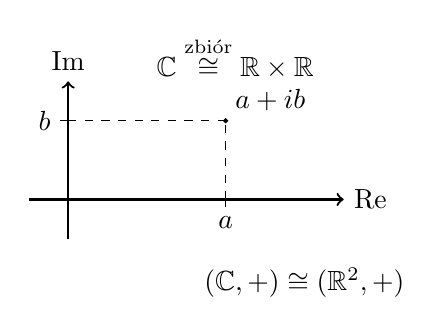
\begin{tikzpicture}
        \draw[->,thick] (-0.5,0)--(3.5,0) node[right]{$\operatorname{Re}$};
        \draw[->,thick] (0,-0.5)--(0,1.5) node[above]{$\operatorname{Im}$};
        \draw (2,0.1)--(2,-0.1) node[below]{$a$};
        \draw (0.1,1)--(-0.1,1) node[left]{$b$};
        \draw[dashed] (2,0)--(2,1); 
        \draw[dashed] (0,1)--(2,1);
        \draw[fill] (2,1) circle[radius=0.025] node[above right]{$a+ib$} ;
        \draw[fill] (1,1.8) circle[radius=0] node[right]{$ \mathbb{C} \overset{\text{zbiór}}{\cong} \mathbb{R} \times \mathbb{R} $};
        \draw[fill] (3,-0.75) circle[radius=0] node[below]{$(\mathbb{C},+) \cong (\mathbb{R}^2,+)$};
    \end{tikzpicture}
\end{minipage}
\begin{ft} 
    $\mathbb{C}$ jest przestrzenią liniową nad $\mathbb{R}$ (izomorifczną z $\mathbb{R}^2$), gdzie 
    $\mathbb{C} \ni a + ib \mapsto \begin{pmatrix} a \\ b \end{pmatrix} \in \mathbb{R}$
\end{ft}
\begin{uw} 
    $r + 0i \overset{\text{ozn}}{=} r$, dla $r \in \mathbb{R}$ (tzn. $\mathbb{R}$ traktujemy jako 
    podciało $\mathbb{C}$). \\ 
    $+,\cdot$ dla liczb rzeczywistych to dodawanie/mnożenie odpowiednich liczb zespolonych
    (tzn. $\mathbb{R}$ to podciało $\mathbb{C}$)
\end{uw} 
\begin{uw} $\dim_\mathbb{R} \mathbb{C} = 2 \quad \dim_\mathbb{C} \mathbb{C} = 1$ \end{uw}
\begin{minipage}[c]{0.65\textwidth}
    \begin{df} Postać trygonometryczna liczby zespolonej: 
        \[ z = a+ib = r\cos \theta + ir\sin \theta = r(cos\theta + i sin \theta) \] \end{df} 
\end{minipage}
\begin{minipage}[c]{0.3\textwidth}
    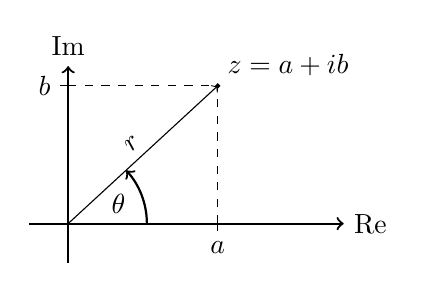
\begin{tikzpicture}
        \draw[->,thick] (-0.5,0)--(3.5,0) node[right]{$\operatorname{Re}$};
        \draw[->,thick] (0,-0.5)--(0,2) node[above]{$\operatorname{Im}$};
        \draw (1.9,0.1)--(1.9,-0.1) node[below]{$a$};
        \draw (0.1,1.75)--(-0.1,1.75) node[left]{$b$};
        \draw[dashed] (1.9,0)--(1.9,1.75); 
        \draw[dashed] (0,1.75)--(1.9,1.75);
        \draw[fill] (1.9,1.75) circle[radius=0.025] node[above right]{$z=a+ib$};
        \draw[->] (0,0)--(1.9,1.75) node[midway,sloped,above]{$r$};
        \draw[->,thick] (1,0) arc[radius=1,start angle = 0, end angle = 42.5];
        \draw[fill] (0.85,0) circle[radius=0] node[above left]{$\theta$};
    \end{tikzpicture}
\end{minipage}
\begin{align*} 
    z &= r(\cos\theta + i\sin\theta)\qquad r,r' \in \mathbb{R}_+ \cup \{0\} \\
    z &= r(\cos\theta' + \sin\theta') \\
    zz' &= (rr')((\cos\theta\cos\theta' - \sin\theta\sin\theta') + 
    i(\cos\theta\sin\theta' + \cos\theta'\sin\theta)) = \\ 
        &= (rr')(\cos(\theta+\theta') + i\sin(\theta+\theta'))
\end{align*}
\begin{df} 
    Jeśli $z = r(\cos\theta + i\sin\theta)$, gdzie $r \in \mathbb{R}_+ \cup \{0\}$, to 
    \begin{align*}
        r & \overset{\text{ozn}}{=} |z| \text{ nazywamy modułem } z.\\
        \theta & \overset{\text{ozn}}{=} \arg z \text{ nazywamy argumentem } z
    \end{align*}
    \footnotetext{$arg: \mathbb{C} \setminus \{0\} \to (\mathbb{R} , +_{\operatorname{mod} 2\pi})$}
\end{df}
\begin{ft} 
    \begin{align*}
        |z \cdot w| &= |z| \cdot |w| \\ 
        \arg(z \cdot w) &= \arg z + \arg w \quad (\operatorname{mod} \ 2\pi) 
    \end{align*}
\end{ft}
\begin{ft} 
    \begin{align*}
        |a + ib| &= \sqrt{a^2 + b^2} \\
        \arg (a+ib) &= \begin{cases} 
                        \operatorname{arctg} \frac{b}{a} & a \neq 0 \\
                        (\operatorname{sgn} b)\frac{\pi}{2} & a = 0
                    \end{cases}
    \end{align*} 
\end{ft} 
\begin{wn} (wzór de Moivre'a) 
    \[ (\cos\theta + i\sin\theta)^n = \cos(n\theta) + i\sin(n\theta) \]  
\end{wn}
\begin{dd} 
    dla $n \in \mathbb{Z}_+$ prosta indukcja,
    dla $n \in \mathbb{Z}_-$ ćwiczenia 
\end{dd} 
\begin{wn}
    \begin{align*}
        z &= r(\cos\theta + i\sin\theta) \\
        z^n &= r^n(\cos(n\theta)+i\sin(n\theta))
    \end{align*}
\end{wn} 
\begin{prz}
    $(1+i)^{100} = -2^{50}$
\end{prz}

\begin{df} 
    \[ e^{x+iy} = e^x(\cos y + i\sin y) \quad \text{ dla } x,y \in \mathbb{R} \] 
    $ \exp: \mathbb{R} \to \mathbb{R} $ \\ 
    $\exp : \mathbb{C} \to \mathbb{C} $
\end{df}
\begin{ft} 
    \[ e^z \cdot e^w = e^{z+w} \quad \text{dla }z,w \in \mathbb{C} \]
\end{ft}
\begin{dd} 
    \begin{align*}
         e^z \cdot e^w &= e^{x +iy} \cdot e^{a + ib} = e^x(\cos y + i \sin y) + e^a(\cos b + i\sin b) \\ 
    &= e^{x+a}(\cos(y+b) + i\sin(y+b)) = e^{(x+a) + i(y+b)} = e^{z+w}  
    \end{align*}
    \hfill \qed
\end{dd} 
\begin{wn} (wzór Eulera) \[ e^{i\pi} + 1 = 0 \] \end{wn}
\subsection{Pierwiastkowanie liczb zespolonych}
$\sqrt{-1} = ?$ \\ 
Chcemy znaleźć funkcję taką, że: 
\begin{align*}
    \sqrt{} &: \mathbb{C} \to \mathbb{C}  \\ 
        &(\sqrt{z})^2 = z  \\ 
        & \text{ciągła} 
\end{align*}
Taka funkcja nie istnieje 
\begin{align*}
    &z = r(\cos\theta + i\sin\theta) \\
    &w^2 = z (\text{myślimy, że} w = \sqrt{z}) \\
    &w = p(cos\varphi + i\sin\varphi) \\
  &\begin{cases} 
        p^2 = r \to p = \sqrt{r} \text{ pierwiastek rzeczywisty} \\
        2*\varphi = \theta \operatorname{mod} 2\pi
    \end{cases}  \\
    &w_1 = \sqrt{r} (\cos\frac{\theta}{2} + i\sin\frac{\theta}{2}) \\ 
    &w_2= \sqrt{r}(\cos\frac{\theta + 2\pi}{2} + i\sin\frac{\theta+2\pi}{2}) \end{align*}
\begin{figure}[!ht]
\centering
    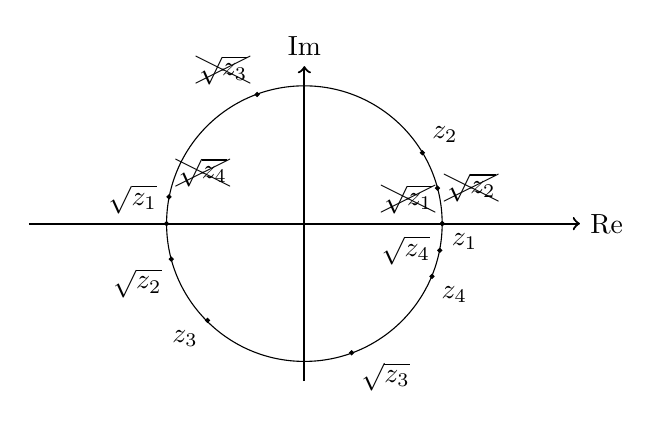
\begin{tikzpicture}
        \draw[->,thick] (-3.5,0)--(3.5,0) node[right]{$\operatorname{Re}$};
        \draw[->,thick] (0,-2)--(0,2) node[above]{$\operatorname{Im}$};
        \draw circle[radius=1.75];
        \draw[fill] (1.75,0) circle[radius=0.025] node[below right]{$z_1$};
        \draw[fill] (1.75,0) circle[radius=0.025] node[above left]{$\xcancel{\sqrt{z_1}}$};
        \draw[fill] (-1.75,0) circle[radius=0.025] node[above left]{$\sqrt{z_1}$};
        \draw[fill] (1.5,0.9) circle[radius=0.025] node[above right]{$z_2$};
        \draw[fill] (1.69,0.45) circle[radius=0.025] node[right]{$\xcancel{\sqrt{z_2}}$};
        \draw[fill] (-1.69,-0.45) circle[radius=0.025] node[below left]{$\sqrt{z_2}$};
        \draw[fill] (-1.23,-1.23) circle[radius=0.025] node[below left]{$z_3$};
        \draw[fill] (-0.6,1.64) circle[radius=0.025] node[above left]{$\xcancel{\sqrt{z_3}}$};
        \draw[fill] (0.6,-1.64) circle[radius=0.025] node[below right]{$\sqrt{z_3}$};
        \draw[fill] (1.62,-0.67) circle[radius=0.025] node[below right]{$z_4$};  
        \draw[fill] (-1.72,0.34) circle[radius=0.025] node[above right]{$\xcancel{\sqrt{z_4}}$}; 
        \draw[fill] (1.72,-0.34) circle[radius=0.025] node[left]{$\sqrt{z_4}$};
    \end{tikzpicture}
    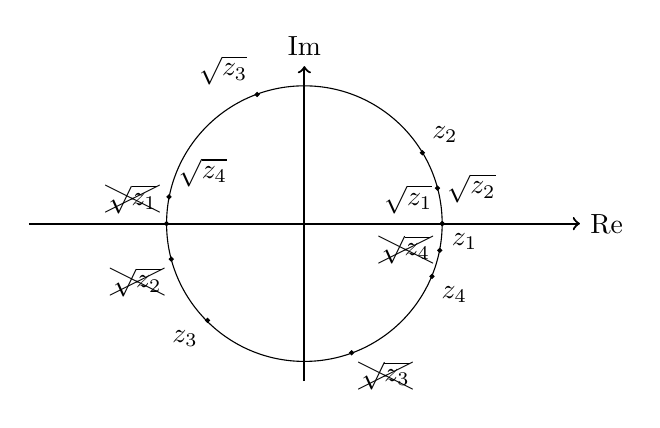
\begin{tikzpicture}
        \draw[->,thick] (-3.5,0)--(3.5,0) node[right]{$\operatorname{Re}$};
        \draw[->,thick] (0,-2)--(0,2) node[above]{$\operatorname{Im}$};
        \draw circle[radius=1.75];
        \draw[fill] (1.75,0) circle[radius=0.025] node[below right]{$z_1$};
        \draw[fill] (1.75,0) circle[radius=0.025] node[above left]{$\sqrt{z_1}$};
        \draw[fill] (-1.75,0) circle[radius=0.025] node[above left]{$\xcancel{\sqrt{z_1}}$};
        \draw[fill] (1.5,0.9) circle[radius=0.025] node[above right]{$z_2$};
        \draw[fill] (1.69,0.45) circle[radius=0.025] node[right]{$\sqrt{z_2}$};
        \draw[fill] (-1.69,-0.45) circle[radius=0.025] node[below left]{$\xcancel{\sqrt{z_2}}$};
        \draw[fill] (-1.23,-1.23) circle[radius=0.025] node[below left]{$z_3$};
        \draw[fill] (-0.6,1.64) circle[radius=0.025] node[above left]{$\sqrt{z_3}$};
        \draw[fill] (0.6,-1.64) circle[radius=0.025] node[below right]{$\xcancel{\sqrt{z_3}}$};
        \draw[fill] (1.62,-0.67) circle[radius=0.025] node[below right]{$z_4$};  
        \draw[fill] (-1.72,0.34) circle[radius=0.025] node[above right]{$\sqrt{z_4}$}; 
        \draw[fill] (1.72,-0.34) circle[radius=0.025] node[left]{$\xcancel{\sqrt{z_4}}$};
    \end{tikzpicture}
    \caption{widać, że pierwiastek nie może być ciągły}
\end{figure}
$\sqrt{}$ na $\mathbb{C}$ jest funkcją wielowartościową.
\begin{ft} 
    Jeśli $ z = r(\cos\theta + i\sin\theta), r \in\mathbb{R}_+$ to $w^n=z$ ma następujące $n$ pierwiastków: 
    \[ w_k = \sqrt[n]{r} (\cos\frac{\theta+2k\pi}{n}+i\sin\frac{\theta+2k\pi}{n}) \quad 
    \text{, dla }k = 0,1,\ldots,n-1 \]
\end{ft}
\begin{prz} $\sqrt{-1} = \pm i$ \end{prz} 
\begin{prz} 
    $\sqrt{i} = ?$ 
    \begin{align*}
        i = (\cos\frac{\pi}{2} &+ i\sin\frac{\pi}{2}) \\
        w_1 = (\cos\frac{5\pi}{4} + i\sin\frac{5\pi}{4})=-\frac{1+i}{2} & \qquad  w_2 = (\cos\frac{\pi}{4} + i\sin\frac{\pi}{4}) = \frac{1+i}{2} 
    \end{align*}
\end{prz}
\begin{uw} $\sqrt[n]{0} = 0 $ \end{uw}
\begin{tw} (zasadnicze twierdzenie algebry) \\ 
    Każdy wielomian zespolony ($P \in \mathbb{C}[x]$) (niestały) ma pierwiastek. 
    \footnotetext{$\mathbb{C}$ jest ciałem algebraicznie domkniętym}
\end{tw} 
\begin{dd}
    Formalny dowód $\rightarrow$ topologia algebraiczna (pojęcie grupy podstawowej). \\ 
    Idea dowodu (nie wprost): \\ 
    $P \in \mathbb{C}[z],\ P(z) = a_n z^n + \ldots + a_1 z + a_0, \ a_in \in \mathbb{C}, a_n \neq 0$
    Zakładamy nie wprost, że $P$ nie ma pierwiastków. 
    $P: \mathbb{C} \xrightarrow{\text{ciągłe}} \mathbb{C} \setminus \{0\} \xrightarrow{\text{ciągłe}} 
    S^1 = \{z \in \mathbb{C} : |z| = 1\}$ \\ 
    $z \mapsto \frac{P(z)}{|P(z)|}$ \\ 
    $F: \overscript{\mathbb{C}}{\cap}{S^1} \to S^1 \quad F(z) = \frac{P(z)}{|P(z)|}$ \\ 
    $fr: \underscript{S^1}{\vertni}{z} \to \underscript{S^1}{\vertni}{\frac{P(z)}{|P(z)|}} \quad
    r \in \mathbb{R}_+,\ |z| = r$ \\
    %rysunek z dużą ilością kułek xD 
    $n(r) \in \mathbb{Z}$ - znakowana liczba nawinięć sznurka na szpulkę nici. (jest niezmienna, 
    dowód właśnie z topologii algebraicznej). \\ 
    $n : \mathbb{R}_+ \mapsto \mathbb{Z}$ jest ono ciągłe, czyli jest stałe! \\ 
    $r: \ P(z) \simeq a \ \to \ n(r) = 0$ \\ 
    $R: \ P(z) \simeq a_n z^n \to n(R) = \deg P$ \hfill \lightning
\end{dd} 
\begin{wn} 
    Jeśli $P \in \mathbb{C}[x]$, to $P$ ma \underline{dokładnie} $\operatorname{deg} P$ pierwiastków 
    (licząc z krotnościami).
\end{wn}
\begin{wn} 
    Każdy wielomian zespolony (niestały) rozkłada się na iloczyn wielomianów liniowcyh \end{wn} 
\begin{dd} 
    $P(z) $ma pierwiastek a.\\ 
    $P(z) = (z-a)Q(z) \quad$ (tw. Bezout'a), a dalej indukcja \hfill \qed
\end{dd} 
\begin{ft} 
    Jesli $P \in \mathbb{R}[x], \ z \in \mathbb{C} $ oraz $P(z) = 0$, to $P(\overline{z}) = 0$. \\ 
    Co więcej krotność $z$ = krotność $\overline{z}$.
\end{ft}
\begin{dd} 
    \begin{align*} 
        &P(x) = a_nx^n + \ldots + a_1x + a_0 \\ 
        0 &= P(z) = a_nz^n + \ldots + a_1z + a_0 \\ 
        \overline{0} &= \overline{a_nz^n + \ldots + a_1z+a_0}\\ 
        0 &= \overline{a_nz^n} + \ldots + \overline{a_1z} + \overline{a_0} \\ 
        0 &= a_n(\overline{z})^n + \ldots + a_1\overline{z} + a_0 = P(\overline{z}) \\
    \end{align*} 
\end{dd} 
\begin{wn} 
    Każdy wielomian rzeczywisty $(P \in \mathbb{R}[x])$ rozkłada się na iloczyn czynników liniowych i kwadratowych
\end{wn}
\begin{dd} 
    \begin{align*} 
        P(x) & = (x-z)(x-\overline{z})Q(x) \quad Q \in \mathbb{C}[x] \\  
        \underscript{P(x)}{\vertin}{\mathbb{R}[x]} & = \underscript{(x^2 - 2ax + (a^2 + b^2))}{\vertin}{\mathbb{R}[x]}Q(x) \\ 
        \text{czyli } Q &\in \mathbb{R}[x] \text{ i kontynuacja indukcyjnie}
    \end{align*}
\end{dd} 
\begin{prz} Zadanie 31 z listy 7 
    \[ \begin{pmatrix} 2\sqrt{3} & -7 \\ 1 & -\sqrt{3} \end{pmatrix}^{100} \cdot \begin{pmatrix} 1 \\ 2 \end{pmatrix} \]
    \begin{align*}    
        \det \begin{pmatrix} 2\sqrt{3} & -7 \\ 1 & -\sqrt{3} \end{pmatrix} = (x-2\sqrt{3})(x+\sqrt{3}) + 7 = \\ 
        = x^2 - \sqrt{3}x + 1 \\ 
        \Delta = 3 - 4 = -1 \\ 
        \sqrt{\Delta} = \pm i \\ 
        x = \frac{\sqrt{3} \pm i}{2} \\ 
    \end{align*}
    \begin{align*}
        &\begin{pmatrix} 2\sqrt{3} & -7 \\ 1 & -\sqrt{3} \end{pmatrix} \cdot \begin{pmatrix} a \\ b \end{pmatrix} = 
        \frac{\sqrt{3} + i}{2} \begin{pmatrix} a \\ b \end{pmatrix} \\
        \begin{cases} 
            2\sqrt{3}a - 7b = \frac{\sqrt{3}+i}{2}a \\
            a - \sqrt{3} b = \frac{\sqrt{3}+i}{2} b
        \end{cases} \\ 
        &\begin{cases} 
            \cancel{\frac{3\sqrt{3}-i}{2} a - 7b = 0}\footnotemark \\ 
            a - \frac{3\sqrt{3}+i}{2}b = 0
        \end{cases} \\ 
        & a = \frac{3\sqrt{3} + i}{2} b \\ 
        \lambda_1 = \frac{\sqrt{3}+i}{2} & \qquad v_1 = \begin{pmatrix} 3\sqrt{3}+i \\ 2 \end{pmatrix} \\ 
        \lambda_2 = \frac{\sqrt{3}-i}{2} & \qquad v_2 = \begin{pmatrix} 3\sqrt 3-i \\ 2 \end{pmatrix} 
    \end{align*}
\end{prz}
\footnotetext{A tam liniowo zalezne krab}
\begin{ft} 
    Jeśli $A \in M_{n\times n}(\mathbb{R})$, zaś $\lambda \in \mathbb{C} \setminus \mathbb{R}$ jest 
    wartością własna $A$, a jej wektor własny to $v \in \mathbb{C}^n$, to $\overline{v} \in \mathbb{C}^n$ jest
    wektorym własnym $A$ dla wartości $\overline{\lambda}$.
\end{ft} 
\begin{dd} 
    $\chi_A \in \mathbb{R}[x]$, więc $\chi_A (\lambda ) = 0 \Rightarrow \chi_A(\overline{\lambda}) = 0$ \\ 
    $Av = \lambda v$ \\ 
    $\overline{Av} = \overline{\lambda v}$ \\ 
    $\overline{A} \cdot \overline{v} = \overline{\lambda} \cdot \overline{v} $ \\ 
    $ A \cdot \overline{z} = \overline{\lambda} \cdot \overline{z}$ \\ 
    czyli $\overline{v}$ to wektory własny dla $\overline{\lambda}$. \hfill \qed
\end{dd} 
\begin{prz} Zadanie 31 lista 7, ale inaczej
    \begin{align*}
        A &= P \begin{pmatrix} \lambda_1 & 0 \\ 0 & \lambda_2 \end{pmatrix} P^{-1} \\
        A^n &= P \begin{pmatrix} \lambda_1^n & 0 \\ 0 & \lambda_2^n \end{pmatrix} P^{-1} = 
        \begin{pmatrix} a_{11} & a_{12} \\ a_{21} & a_{22} \end{pmatrix} \\ 
        a_{ij} &= \alpha_{ij} \lambda_1^n + \beta_{ij} \lambda_2^n \text{, gdzie } \alpha_{ij},\beta_{ij} 
        \text{ nie zależą od } n. \\
        \lambda_1 &= \frac{\sqrt{3}+i}{2}, \quad \lambda_2 = \frac{\sqrt{3}-i}{2} \\ 
        &\begin{cases}
            a_n = \alpha (\frac{\sqrt{3}+i}{2})^n + \alpha' (\frac{\sqrt{3}-i}{2})^n \\ 
            b_n = \beta (\frac{\sqrt{3}+i}{2})^n + \beta' (\frac{\sqrt{3}-i}{2})^n 
        \end{cases} \\
        &\underline{n=0} \\ 
        &\begin{cases}
            1 = a_0 = \alpha + \alpha' \\ 
            2 = b+0 = \beta + \beta' 
        \end{cases} \\ 
        &\underline{n=1} \\ 
        &\begin{cases}
            2\sqrt{3} - 14 = a_2 = \alpha (\frac{\sqrt{3}+i}{2}) + \alpha' (\frac{\sqrt{3}-i}{2}) \\ 
            1 - 2\sqrt{3} = b_2 = \beta (\frac{\sqrt{3}+i}{2}) + \beta' (\frac{\sqrt{3}-i}{2})
        \end{cases} \\ 
        &\text{Z tego da się obliczyć } \alpha,\alpha',\beta,\beta'
    \end{align*}
\end{prz} 
\begin{uw} $a_{ij} = \alpha_{ij} \lambda_1 ^n + \beta_{ij} \lambda^n_2$ opisuje nam jak $a_{ij}$ będzie się 
    zachowywać ( o tym który z czynników $\lambda_1,\lambda_2$ dominuje decyduje ich moduł) 
    (opisuje asymptotykę). \end{uw}
\begin{uw} Pytanie z publiczności (jakby ktoś chciał je poznać to proszę do Mateusza Rzepeckiego).\\
    $\lambda = r(\cos\theta + i\sin\theta)$ \\ 
    $\overline\lambda = r(\cos\theta-i\sin\theta)$ \\ 
    $ \alpha = s(\cos\varphi + i\sin\varphi)$ \\ 
    $a_n = \alpha (\lambda)^n + \beta (\overline\lambda)^n \in \mathbb{R}$ dla dowolnego n \\
    $\overline\beta \lambda^n + \beta(\overline\lambda)^n \in \mathbb{R}$, odejmując otrzymujemy: \\ 
    $(\alpha - \overline\beta) \lambda^n \in \mathbb{R}$ dla dowolnego n, czyli $\alpha = \overline\beta$\\ 
    $a_n = \alpha \lambda^n + \overline\alpha (\overline\lambda)^n = 2 \operatorname{Re}(\alpha\lambda^n)$ \\ 
    $a_n = 2sr^n \cos(\varphi + n\theta)$
\end{uw} 
\section{Suma prosta} 
\begin{minipage}[c]{0.5\textwidth}
$V$ \\ 
baza $B = (b1,\ldots,b_n)$ \\ 
$F: V \to V$ \\ 
$W = \operatorname{Lin} \{ b_1,\ldots,b_k\} < V$ \\ 
$W' = \operatorname{Lin}\{ b_{k+1},\ldots,b_n\} < V$ 
\end{minipage}%
\begin{minipage}[c]{0.4\textwidth}
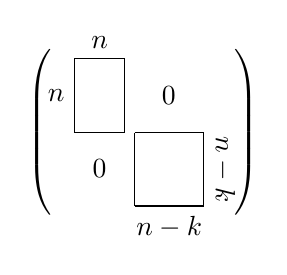
\begin{tikzpicture}
    \matrix[matrix of nodes,nodes in empty cells, left delimiter = (, right delimiter = )] (m)
    { 
         &  &  & & & &\\
         &  &  & & 0& &\\
         &  &  & & & &\\
         &  &  & & & &\\ 
         &  0&  & & & &\\
         &  &  & & & &\\
    };
    \draw (m-1-1.north) -- (m-3-1.south) node[midway, left]{$n$}; 
    \draw (m-1-1.north) -- (m-1-3.north) node[midway, above]{$n$};
    \draw (m-3-1.south) -- (m-3-3.south);
    \draw (m-3-3.south) -- (m-1-3.north);

    \draw (m-3-3.south east) -- (m-3-6.south east);
    \draw (m-3-6.south east) -- (m-6-6.south east) node[midway,above,sloped]{$n-k$};
    \draw (m-6-6.south east) -- (m-6-3.south east) node[midway,below]{$n-k$};
    \draw (m-6-3.south east) -- (m-3-3.south east);
\end{tikzpicture}
\end{minipage} \\
Niech $W,W' - F -$ niezmiennicze. \\
$F: V \to V \rightsquigarrow F_{|_W}: W \to W, \ F_{|_{W'}}: W' \to W'$ \\
$V = W \oplus W'$ (suma prosta podprzestrzeni $W$ i $W'$).
\begin{df} 
    Przestrzeń liniowa $V$ jest \underline{sumą prostą} przestrzeni $V_1,\ldots,V_n < V$ \\ 
    (ozn. $V = V_1 \oplus \ldots \oplus V_n = \underset{i=1}{\overset{n}{\oplus}} V_i$), jeśli 
    każdy wektor $v \in V$ przedstawia się \underline{jednoznacznie} w postaci $v = v_1+\ldots+v_n$, gdzie 
    $v_i \in V_i$.
\end{df} 
\begin{prz} 
    $B = (b_1,\ldots,b_n)$ - baza $V$ \\ 
    $V = \operatorname{Lin}\{b_1\} \oplus \ldots \oplus \operatorname{Lin}\{b_n\}$
\end{prz}
\begin{prz} 
    $B = (b_1,\ldots,b_n)$ - baza $V$ \\ 
    $V = \operatorname{Lin}\{b_1,\ldots,b_k\} \oplus \operatorname{Lin}\{b_{k+1},\ldots,b_n\}$ \\ 
    $V \ni v = (\alpha_1 b_1 + \ldots + \alpha_k b_k) + (\alpha_{k+1} b_{k+1} + \ldots + \alpha_n b_n)$ 
\end{prz} 
\begin{prz} 
    \begin{align*}
        \mathbb{R}[x] = \{ P \in \mathbb{R}[x] : P(-x) &= P(x) \} = \operatorname{Lin}\{1,x^2,x^4,\ldots\} \\ 
        &\oplus \\ 
        \{ P \in \mathbb{R}[x] : P(-x) &= -P(x) \}  \\ 
    \end{align*}
    \[P(x) = \frac{P(x)+P(-x)}{2} + \frac{P(x) - P(-x)}{2} \]
\end{prz}
\begin{prz} 
    $\mathbb{R}^3 = \left\{ \begin{pmatrix} x \\ y \\ z \end{pmatrix}: x + y + z = 0 \right\} \oplus 
    \left\{ t \begin{pmatrix} 1 \\ 1 \\ 1 \end{pmatrix}, t \in \mathbb{R} \right\} $
\end{prz}
\begin{df} 
    Podprzestrzenie $V_1,\ldots,V_n < V$ nazywamy lnz jeśli: 
    \[ (\forall v_1 \in V_1,\ldots,v_n \in V_n) \quad v_1 + \ldots +v_n = 0 \Rightarrow v_1 = \ldots = v_n = 0 \]
\end{df} 
\begin{prz} 
    $V_i = \operatorname\{v_i\}$ \\ 
    $V_1,\ldots,V_n$ lnz $\Leftrightarrow v_1,\ldots,v_n$ lnz 
\end{prz}
\begin{lem}
    $V_1,\ldots,V_n < V$ lnz $\Leftrightarrow \forall i (V_i \cap (V_1+\ldots+\widehat{V_i} + \ldots + V_n) = \{0\})$
    \begin{dd} \hfill 
        \begin{itemize} 
            \item[$\Rightarrow$] $v_i \in V_i \setminus \{0\}$, gdyby \\ 
                $v_i = v+1 + \ldots + \widehat{v_i} + \ldots + v_n$ \\ 
                $v_1 + \ldots - v_i + \ldots + v_n = 0$ \hfill \lightning
            \item[$\Leftarrow$] wprost \\ 
                $v_1 + \ldots + v_n = 0$ \\ 
                $v_i = -v_1 - v_2 - \ldots - \widehat{v_i} - \ldots - v_n$ \\ 
                $V_i \cap (V_1 + \ldots + \widehat{V_i}+ \ldots + V_n) = \{0\}$ \\ 
                czyli $v_i = 0 $ dla dowolnego $i$. \hfill \qed
        \end{itemize}
    \end{dd} 
\end{lem}
\begin{wn} 
    $V_1,V_2 < V$ lnz $\Leftrightarrow V_1 \cap V_2 = \{0\}$
\end{wn} 
\begin{df}[nobreak = true]
    Jeśli $V_1,\ldots,V_n$ to dowolne przestrzenie liniowe nad $K$, to \underline{produktem} $V_1,\ldots,V_n$ 
    nazywamy zbiór: 
        \[ V_1 \times V_2 \times \ldots \times V_n \text{, z działaniami }\] 
     \begin{align*} 
        (v_1,\ldots,v_n)+(v_1',\ldots,v_n') &= (v_1 + v_1',\ldots,v_n+v_n') \\ 
        \alpha (v_1,\ldots,v_n) &= (\alpha v_1,\ldots,\alpha v_n)
    \end{align*}
\end{df} 
\begin{ft} 
    $V_1,\ldots,V_n$ jest przestrzenią liniową
\end{ft} 
\begin{dd} 
    ćw 
\end{dd} 
\begin{przy} \hfill 
    \begin{itemize} 
        \item $\mathbb R^2 = \mathbb R \times \mathbb R$
        \item $K^n = \underbrace{K \times K \times \ldots \times K}_{n}$
    \end{itemize} 
\end{przy} 
\begin{ft} 
    Niech $V_1,\ldots,V_n < V$. Wówczas NWSR:
    \begin{enumerate}[(1)]
        \item $V = V_1 \oplus \ldots \oplus V_n$
        \item $V_1,\ldots,V_n$ lnz oraz $V_1+\ldots,V_n=V$
        \item $\phi : V_1 \times V_2 \times \ldots \times V_n \to V$ jest izomorfizem \\
        Jeśli $\dim V < \infty$
        \item $V_1,\ldots,V_n$ lnz oraz $\dim V_1 + \ldots + \dim V_n = \dim V$ 
        \item $V_1+\ldots + V_n = V$ oraz $\dim V_1 + \ldots + \dim V_n = \dim V$
    \end{enumerate}
\end{ft} 
\begin{lem} \label{indeksior}
    $\dim (V_1 \times \ldots \times V_n) = \dim V_1 + \ldots + \dim V_n$
    \begin{dd} 
        $(0,\ldots,0,b_{i,i_k},0,\ldots,0),\ 1 \le i_k \le \dim V_k$
        jest bazą. $V_1 \times \ldots \times V_n$. Reszta zostawione jako ćwiczenie.
        \footnotetext{$b_{k,1},\ldots,b_{k,\dim V_k}$ jest bazą $V_k$}
    \end{dd} 
\end{lem} 
\begin{dd}  \hfill
    \begin{itemize} 
        \item[$(1) \Rightarrow (2)$] $V_1,\ldots,V_n$ lnz: \\ 
            $v_1 + \ldots + v_n = 0$. Z jednoznaczności $v_i = 0$. \\ 
            $V_1 + \ldots + V_n = V$: \\ 
            $V \ni v = v_1 + \ldots v+n$ z def.
        \item [$(2) \Rightarrow (3)$] $\phi$ jest liniowe. \\ 
            $\phi$ jest "na", bo $V_1+\ldots+V_n = \operatorname{Im} \phi = V$ \\ 
            $\phi$ jest różnowartściowe, bo $\ker \phi = \{ (v_1,\ldots,v_n): v_1+\ldots+v_n = 0\} = 
            \{(0,\ldots,0)\}$, bo $(V_1,\ldots,V_n)$ są lnz. 
        \item [$(3) \Rightarrow (1)$] $v \in V$ \\ 
            $v_i \in V_i$, takie, że $v = (v_1 + \ldots + v_n)$ \\ 
            $v = \phi (v_1,\ldots,v_n)$ \\ 
            $\phi$ jest izomorfizmem ,więc $\exists ! (v_1,\ldots,v_n)$ 
        \item [$(3) \Leftrightarrow (4)$] 
        \item [$(3) \Leftrightarrow (5)$] tw. o indeksie dla $\phi$: \\ 
            $\dim V_1 + \ldots \dim V_n = \dim \ker \phi + \dim \operatorname{Im} \phi = 
            \dim \ker \phi + \dim (V_1+\ldots+V_n)$
            \begin{align*} 
                \dim V_1 + \ldots V_n &= \dim (V_1 + \ldots + V_n) \\ 
                &\Updownarrow  \\ 
                \ker \phi &= \{ 0\} \\ 
                \dim (V_1 + \ldots + V_n) &= \dim V \\ 
                &\Updownarrow \\ 
                V &= V_1 + \ldots V_n \\
                \phi \text{ jest} &\text{ izomorfizmem} \\ 
                 &\Updownarrow \\ 
                \ker \phi = \{ 0\} &\text{ oraz } \operatorname{Im} \phi = V
            \end{align*}  
    \end{itemize} 
\end{dd} 
\begin{wn} 
    Jeśli $V_1,V_2 < V, \ \dim V < \infty$ to NWSR:
    \begin{enumerate}[(1)]
        \item $V = V_1 \oplus V_2$
        \item $V_1 \cap V_2 = \{ 0\}$ oraz $V_1 + V_2 = V$
        \item $V_1 \cap V_2 = \{ 0\}$ oraz $\dim V_1 + \dim V_2 = \dim V$ 
        \item $V_1 + V_2 = V$ oraz $\dim V_1 + \dim V_2 = \dim V$
    \end{enumerate} 
\end{wn}
\begin{lem} 
    Dla dowolnej $W < V$ istnieje $W' < V$ (tw. o podprzestrzeni dopełniczej) taka, że \[V = W \oplus W'\]
    \begin{dd} Był na cwiczeniach \end{dd} 
\end{lem} 
\begin{df} 
    Niech $F: V \to V,\ W < V \ W$ jest $F-$ niezmiennicza, jesli \[ (\forall w \in W) (F(w) \in W)\]
\end{df}
\begin{ft} 
    $F: V \to V,\ \lambda_1,\ldots,\lambda_n$ - parami różne wartości własne, to $V_{\lambda_1},\ldots,
    V_{\lambda_n}$ są lnz oraz są $F-$ niezmiennicze.
\end{ft} 
\begin{wn} 
    $V = V_{\lambda_1} \oplus \ldots \oplus V_{\lambda_n} \oplus W$ dla pewnej $W < V$
\end{wn} 
\begin{ft} 
    $F: V \to V$ liniowe \\ 
    $V_1,\ldots,V_n$ - $F-$ niezmiennicze \\ 
    $V = V_1 \oplus \ldots \oplus V_n$ 
    Wówczas $\chi_F = \chi_{F|{V_1}} \cdot \ldots \cdot \chi_{F|V_n}$
\end{ft} 
\begin{dd} ~\\ 
    $B_i$ - baza $V_i$ \\ 
    $B = \cdot \hspace{-7.5pt}\bigcup B_i$ - baza $V$ %xDDDDDDDDDDDDDDDDDDDDDDDDDDDDDDDDDDDDDDd
    \[ m_B^B (F) = 
        \begin{pmatrix} 
            m_{B_1}^{B_1} (F_{|V_1}) & & &  \\ 
                                     &  m_{B_2}^{B_2} (F_{|V_2}) & & \\ 
                                     & & \ddots & \\ 
                                     & & &   m_{B_n}^{B_n} (F_{|V_n}) 
        \end{pmatrix} 
    \]
    \[ \det (m_B^B (F) - xI) = \prod_{i=1}^n \det (m_{B_i}^{B_i} (F_{|V_i}) -xI)\]
\end{dd} 
\begin{ft} 
    Jeśli $F: V \to V$ liniowy, $W$ jest $F-$ niezmienniczą podprzestrzenią $V$ oraz $\overline F: V/_{W} \to V/_W$ \\ 
    zdefiniowane $\overline F (v+W) = F(v) + W$, to $\chi_F = \chi_{F|_w} \cdot \chi_{\overline F}$
\end{ft} 
\begin{dd} ~\\ 
    $\overline F$ dobrze zdefiniowane 
    \begin{align*}
        v+1 + W &= v_2 + W  \\ 
                &\Updownarrow \\
        v_1 - v_2 &\in W  \\ 
                  &\Downarrow  \\ 
        F(v_1) - F(v_2) &\in W \\ 
                        &\Updownarrow \\
        F(v_1) + W &= F(v_2) + W
    \end{align*} 
    $v_1 - v_2 \in W \Rightarrow F(v_1 - v_2) \in W$ \\ 
    $\overline F$ liniowe (ćw) \\ 
    $\mathcal B = (b_1,\ldots,b_k)$ - baza W \\ 
    $\mathcal B' = (b_1,\ldots,b_k,b_{k+1},\ldots,b_n)$ - baza V \\ 
    baza $V/_W = \overline B (b_{k+1}+W,\ldots,b_n+W)$ \\ 
    $m_{B'}^{B'} (F) = \begin{pmatrix} m_B^B (F_{|W}) & \ast \\ 0 & m_{\overline B}^{\overline B}(\overline F) \end{pmatrix}$ \\
    $\det(m_{B'}^{B'} (F) - xI) = \det (m_B^B (F_{|{W}}) - Ix) \cdot 
    \det (m_{\overline B}^{\overline B} (\overline F) - xI)$
\end{dd}
\section{Diagonalizacja macierzy} 
\begin{enumerate} 
    \item Wartość, wektory własne $\to$ diagonalizować 
    \item Przeszkoda 1: $\chi_F$ ma za mało pierwiastków \\ 
        Rozwiązanie: $\mathbb C$ zamiast $\mathbb R$
    \item Przeszkoda 2: za małe przestrzenie własne ($\dim V_\lambda < $ krotność $\lambda$)\\
        Rozwiązanie (częściowe): \underline{tw. Jordana}: \\
        Każda macierz można zapisać w postaci 
        \[ PJP^{-1}, \ \text{gdzie } J = \begin{pmatrix} J_1 & & \\ & \ddots & \\ & & J_k \end{pmatrix}
        \text{, a } J_i = \begin{pmatrix} \lambda_i & 1 & & & \\ & \ddots & \ddots & & \\ 
            & & \ddots & 1 \\ & & &  \lambda_i \end{pmatrix}
        \]
    \item Ulubione macierze: macierze symetryczne. \\
        \underline{Tw. spektralne}: Macierz symetryczna nad $\mathbb R$ zawsze się diagonalizuje
        (i to nad $\mathbb R$) i do tego można wybrać bazę wektorów własnych złożoną z wektorów 
        parami prodopadłych.
    \item Co z macierzami prostokątnymi? subsytut diagonalizowalności dla macierzy prostokątnych $=$ rozkład SVD
\end{enumerate} 
\subsection{Po co diagonalizować}
\begin{enumerate} 
    \item Podnosić macierze do wysokich potęg. (np. macierz $A$ reprezentuje pewien proces który iterujemy 
        $n-$ krotnie.)
    \item $ A = P \begin{pmatrix} \lambda_1 & & \\ & \ddots & \\ & & \lambda_n \end{pmatrix} P^{-1} 
        \approx P \begin{pmatrix} \lambda_1 & & & & & \\ 
                                    & \ddots & & & & \\ 
                                    & & \lambda_k & & & \\ 
                                    & & & 0 & & \\ 
                                    & & & & \ddots & \\ 
                                    & & & & & 0 \end{pmatrix} P^{-1}$.\\ 
                                    Kompresja danych, jezeli $\lambda_1 > 
                                    \lambda_2 > \ldots > \lambda_n$, to można zgubić mniejsze.
\end{enumerate} 
\subsection{Rozwiązywanie rekurencji} 
$\begin{cases} 
    a_{n+1} = 5a_n - 6a_{n-1} \\ 
    a_1 = 2 \\ 
    a_0 = 3
\end{cases}$ \\ 
$\begin{pmatrix} 
    a_{n+1} \\ a_n
    \end{pmatrix} = \begin{pmatrix} 5 & -6 \\ 1 & 0 \end{pmatrix} \cdot \begin{pmatrix} a_n \\ a_{n-1}
    \end{pmatrix}$ \\ 
$\begin{pmatrix} a_1 \\ a_0 \end{pmatrix} \mapsto \begin{pmatrix} a_2 \\ a_1 \end{pmatrix} 
\mapsto \begin{pmatrix} a_3 \\ a_2 \end{pmatrix} \mapsto \ldots$  \\ 
$\begin{pmatrix} 
    a_{n+1} \\ a_n
    \end{pmatrix} = \begin{pmatrix} 5 & -6 \\ 1 & 0 \end{pmatrix}^n \cdot \begin{pmatrix} a_1 \\ a_0
    \end{pmatrix}$ \\
$\lambda_1 = 2 \quad v_1 = \begin{pmatrix} 2 \\ 1 \end{pmatrix}$ \\ 
$\lambda_2 = 3 \quad v_2 = \begin{pmatrix} 3 \\ 1 \end{pmatrix}$ \\ 
$\begin{pmatrix} 
    a_{n+1} \\ a_n
    \end{pmatrix} = \begin{pmatrix} 2 & 3 \\ 1 & 1 \end{pmatrix} 
    \cdot \begin{pmatrix} 2^n &  \\  & 3^n \end{pmatrix} 
    \cdot \begin{pmatrix} 2 & 3 \\ 1 & 1 \end{pmatrix}^{-1}
    \cdot \begin{pmatrix} 2 \\ 3 \end{pmatrix}$ \\
Dla dowolnych warunków początkowych mamy: \\
$\begin{pmatrix} 
    a_{n+1} \\ a_n
    \end{pmatrix} = \begin{pmatrix} 2 & 3 \\ 1 & 1 \end{pmatrix} 
    \cdot \begin{pmatrix} 2^n &  \\  & 3^n \end{pmatrix} 
    \cdot \begin{pmatrix} 2 & 3 \\ 1 & 1 \end{pmatrix}^{-1}
    \cdot \begin{pmatrix} \alpha \\ \beta \end{pmatrix}$ \\
\noindent\rule{\textwidth}{0.4pt}\\ 
$b_{n+1} = 4 b_n - 4 b_{n-1}$ \\
$\begin{pmatrix} 
    b_{n+1} \\ b_n
    \end{pmatrix} = \begin{pmatrix} 4 & -4 \\ 1 & 0 \end{pmatrix} \cdot \begin{pmatrix} b_n \\ b_{n-1}
    \end{pmatrix}$ \\ 
$\begin{pmatrix} 
    b_{n+1} \\ b_n
    \end{pmatrix} = \begin{pmatrix} 4 & -4 \\ 1 & 0 \end{pmatrix}^n \cdot \begin{pmatrix} b_1 \\ b_0
    \end{pmatrix}$ \\ 
$\lambda_1 = \lambda_2 = 2$\\ 
$ \dim V_2 = 1$ \\ 
$\begin{pmatrix} 4 & -4 \\ 1 & 0 \end{pmatrix} = P \begin{pmatrix} 2 & 1 \\ 0 & 2 \end{pmatrix} P^{-1}$ \\ 
$\begin{pmatrix} 4 & -4 \\ 1 & 0 \end{pmatrix}^n = P \begin{pmatrix} 2 & 1 \\ 0 & 2 \end{pmatrix}^n P^{-1}$ 
\begin{lem}
    $ \begin{pmatrix} \lambda & 1 \\ 0 & \lambda \end{pmatrix}^n = \begin{pmatrix} \lambda^n & n\lambda^{n-1} \\ 
    0 & \lambda^n \end{pmatrix}$ 
\begin{dd} 
    prosta indukcja na ćwiczenia
\end{dd} 
\end{lem} 
$\begin{pmatrix} 4 & -4 \\ 1 & 0 \end{pmatrix}^n = P \begin{pmatrix} 2^n & n2^{n-1} \\ 0 & 2^n 
\end{pmatrix} P^{-1}$ \\ 
$b_n = \begin{pmatrix} 0 & 1 \end{pmatrix} P \begin{pmatrix} 2^n & n2^{n-1} \\ 0 & 2^n \end{pmatrix} P^{-1} 
\begin{pmatrix} b_1 \\ b_0 \end{pmatrix}$ \\ 
$b_n = c_1 2^n + \frac{c_2}{2} n 2^n$
\subsection{Łańcuch Markowa (proces Markowa z czasem dyskretnym)}
(probabilistyczny automat skończony) \\ 
(błądzenie losowe po grafie skierowanym) \\
\textbf{Zadanie}:
Rzucamy $100$ razy monetą. Jakie jest prawdopodobieństwo, że wypadną (w którymkolwiek momencie) 3 orły pod rzad?\\
\begin{minipage}[c]{0.5\textwidth}
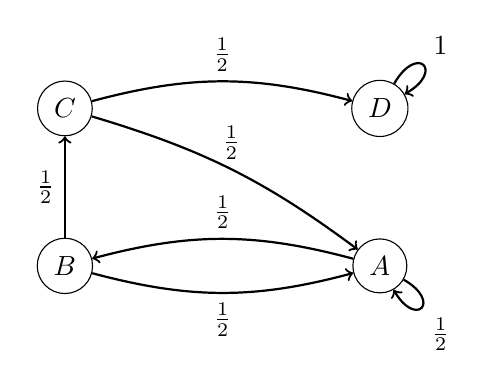
\begin{tikzpicture}
    \node[shape=circle,draw=black] (A) at (4,0) {$A$};
    \node[shape=circle,draw=black] (B) at (0,0) {$B$};
    \node[shape=circle,draw=black] (C) at (0,2) {$C$};
    \node[shape=circle,draw=black] (D) at (4,2) {$D$};
    \path[->,thick] (A) edge [out=330,in=300,looseness=8] node[below right]{$\frac{1}{2}$} (A);
    \path[->,thick] (A) edge [bend right = 15] node[above]{$\frac{1}{2}$} (B);
    \path[->,thick] (B) edge [bend right = 15] node[below]{$\frac{1}{2}$} (A);
    \path[->,thick] (B) edge node[left]{$\frac{1}{2}$} (C);
    \path[->,thick] (C) edge [bend left = 10] node[above]{$\frac{1}{2}$} (A);
    \path[->,thick] (C) edge [bend left = 15] node[above]{$\frac{1}{2}$} (D);
    \path[->,thick] (D) edge [out=60,in=30,looseness=8] node[above right]{$1$} (D);
\end{tikzpicture} 
\end{minipage}%
\begin{minipage}[c]{0.5\textwidth} 
    \centering
    \begin{tabular}{ |r| c| } 
        \hline
        ostatnie rzuty & sytuacja \\
        \hline 
        \ldots R & $A$ \\
        \ldots RO & $B$ \\
        \ldots ROO & $C$ \\ 
        \ldots OOO & $D$ \\
        \hline
    \end{tabular} 
\end{minipage}  \\ 
%-------------------------------------
Loop$a_n=$ prawdopodobieństwo znalezienie się w $A$ w $n$ krokach \\ 
$b_n=$ prawdopodobieństwo znalezienie się w $B$ w $n$ krokach \\ 
$c_n=$ prawdopodobieństwo znalezienie się w $C$ w $n$ krokach \\ 
$d_n=$ prawdopodobieństwo znalezienie się w $D$ w $n$ krokach  \\ 
$a_{n+1} = \frac{1}{2} a_n + \frac{1}{2} b_n + \frac{1}{2} c_n$ \\ 
$b_{n+1} = \frac{1}{2} a_n$ \\ 
$c_{n+1} = \frac{1}{2} b_n$ \\ 
$d_{n+1} = \frac{1}{2} c_n + d_n$ \\
$\begin{pmatrix} a_{n+1} \\ b_{n+1} \\ c_{n+1} \\ d_{n+1} \end{pmatrix} = 
\begin{pmatrix} \frac{1}{2} & \frac{1}{2} & \frac{1}{2} & 0 \\ 
                \frac{1}{2} & 0 & 0 & 0 \\ 
                0 & \frac{1}{2} & 0 & 0 \\ 
            0 & 0 & \frac{1}{2} & 1 \end{pmatrix} \cdot 
            \begin{pmatrix} a_n \\ b_n \\ c_n \\ d_n \end{pmatrix}$ \\ 
$X_{n+1} = M X_n$ \\ 
$M = (m_{ij})$ ma następujące właśności: 
\begin{enumerate} 
    \item $0 \le m_{ij} \le 1$ 
    \item $\sum\limits_{i=1}^n m_{ij} = 1$ (suma kolumy), dla wszystkich j
\end{enumerate} 
tzw. (lewa)\footnote{prawa byłaby jakby wiersze się sumowały} macierz stochastyczna 
$X_{100} = M^{100} X_0$ \\ 
$d_{100} = \begin{pmatrix} 0 & 0 & 0 & 1 \end{pmatrix} M^{100} \begin{pmatrix} 1 \\ 0 \\ 0 \\ 0 \end{pmatrix}$ \\
Graf $(V,E)$ skierowany, skończony z wagami $p_i \in [0,1]$ na krawędzi $e_i$ t. że 
$f(v) = \sum\limits_i p_i = 1$ (poczatek krawędzi $e_i$ to $v$)
Błądzimy losowo po grafie.
\begin{ft} 
    $A$ jest lewą macierzą stochastyczną wtedy i tylko wtedy, gdy 
    $\begin{pmatrix} 1 \\ 1 \\ \vdots \\ 1 \end{pmatrix}$
    jest wektorem własnym dla wartości własnej $1$ dla macierzy $A^\top$ oraz $a_{ij} \ge 0$.
\end{ft} 
\begin{dd} 
    $\begin{pmatrix} 1 & \ldots & 1 \end{pmatrix} A = \begin{pmatrix} 1 & \ldots & 1 \end{pmatrix} \quad /^\top$
\end{dd} 
\begin{ft} $(AB)^\top = B^\top A^\top$ \end{ft} 
\begin{ft} $\chi_A = \chi_{A^\top}$ \end{ft} 
\begin{dd} $\det ((A-xI)^\top) = det(A-xI)$ \end{dd} 
\begin{wn} Jeśli $A$ jest lewa stochastyczna to $A$ ma wartość własną $1$. Ponadto dla dowolnej wartości własnej 
    $\lambda$ macierzy $A$ zachodzi $|\lambda| \le 1$ \end{wn}
\begin{dd} 
    Wystarczy pokazać dla $A^\top$. 
    \[ A^\top \begin{pmatrix} z_1 \\ z_2 \\ \vdots \\ z_n \end{pmatrix} = 
    \lambda \begin{pmatrix} z_1 \\ z_2 \\ \vdots \\ z_n \end{pmatrix}, \quad z_i \in \mathbb C\]
    $ \sum a_{ij} z_j = \lambda z_j $, weźmy $z_k$ taki, że $|z_k|$ maksymalny. \\ 
    $|z_k| = |z_k| \sum c_{ij} \ge \sum a_{ij} |z_j| \ge | \sum a_{ij} z_j| = |\lambda z_k| = |\lambda| |z_k|$, 
    czyli $|z_k| \ge |\lambda| |z_k|$, czyli $|\lambda| \le 1$.
\end{dd} 
\subsection{PageRank}
$\sim$ jakie jest prawdopodobieństwo, że trafimy na daną stronę losowo poruszając się po sieci\\ 
$M \in M_{N \times N}, \quad N=$ liczba stron w sieci \\ 
$m_{ij} = \begin{cases} \frac{0.15}{N} & \text{, jeśli strona } j \text{ nie linkuje do } i \\ 
\frac{0.15}{N} + \frac{0.85}{n_j} & \text{, jeśli strona } j \text{ linkuje do } i \ (n_j=\text{ liczba linków na stronie}) \end{cases}$ \\ 
Mamy nadzieję na: 
$ \lim\limits_n M^n \begin{pmatrix} \frac{1}{N} \\ \vdots \\ \frac{1}{N} \end{pmatrix} = $ pagerank
\begin{tw}[Perrona-Frobeniusa]
    Niech $M$ będzie macierzą dodatnią (tzn $m_{ij} > 0$). Wówczas istnieje takie $r \in \mathbb R_+$, że:
    \begin{enumerate}[(1)]
        \item $r$ jest wartością własną $M$
        \item $ |\lambda| < r$ dla każdej wartości własnej $\lambda \neq r$ 
        \item $r$ jest 1-krotna 
        \item $r$ ma dodatni wektor własny (tzn. wektor o wspołrzędnych dodatnich)
    \end{enumerate} 
\end{tw} 

\section{Dowód tw. Jordana} 
\footnotetext{Ciała algebraincze domknięte muszą być nieskończone.}
\begin{tw}[Jordana]
    Każda macierz,w ciele algebraicznie domkniętym, da się zapisać w postaci 
    \[ P\begin{pmatrix} J_1 & & \\ & \ddots & \\ & & J_k \end{pmatrix}P^{-1}
    \text{, gdzie } J_i = \begin{pmatrix} \lambda_i & 1 & & & \\ & \ddots & \ddots & & \\ 
    & & \ddots & 1 \\ & & &  \lambda_i \end{pmatrix}
    \]
\end{tw} 
\[ A = PJP^{-1}, \ \text{gdzie } J = \begin{pmatrix} J_1 & & \\ & \ddots & \\ & & J_k \end{pmatrix}
\text{, a } J_i = \begin{pmatrix} \lambda_i & 1 & & & \\ & \ddots & \ddots & & \\ 
    & & \ddots & 1 \\ & & &  \lambda_i \end{pmatrix}
\]
$\chi_A^{(x)} = \prod\limits_{i=1}^k (\lambda_i - x)^{m_i}$ \\ 
$V$ - przestrzeń liniowa nad $\mathbb C$ (lub innym algebraicznie domkniętym ciałem) \\
cel 1: 
$V = V_1 \oplus \ldots \oplus V_k$, tak, że $V_i$ jest F-niezmiennicze. \\ 
$V_\lambda = \ker(F-\lambda I) \subset \ker (F - \lambda I)^2 \subset \ker(F - \lambda I)^3 \subset \ldots$ 
(stabilizuje się od pewnego miejsca) 
\begin{ft} 
        Jeśli $\ker(F - \lambda I)^k = \ker (F - \lambda I)^{k+1}$, to $\ker(F - \lambda I)^k = \ker(F - \lambda I)^{k+j}$
\end{ft} 
\begin{dd} 
    Wystarczy pokazać, że $\ker (F - \lambda I)^{k+1} \supset \ker(F - \lambda I)^{k+2}$ \\ 
    $v \in \ker (F - \lambda I)^{k+2}$ \\ 
    $(F - \lambda I)^{k+2} (v) = 0$ 
    $(F - \lambda I)^{k+1} ((F - \lambda I) (v)) = 0$, czyli $(F - \lambda I)v \in 
    \ker(F-\lambda I)^{k+1} = \ker(F - \lambda I)^k$ \\ 
    zatem $0 = (F - \lambda I)^k ((F - \lambda I)v) = (F - \lambda I)^{k+1} (v)$, czyli 
    $v \in \ker(F - \lambda I)^{k+1}$
\end{dd} 
\begin{df} 
    Przestrzenią pierwiastkową odwzorowania $F: V \to V$ nazywamy
    \[V^\lambda = \ 
        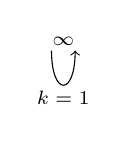
\begin{tikzpicture}[scale = 0.3,baseline]
            \node at (0.5,1.4) {\scriptsize$\infty$};
            \node at (0.5,-1) {\scriptsize$k=1$};
            \path[->] (0,1) edge [bend right = 90,looseness=5] (1,1);
        \end{tikzpicture} \ 
    \ker (F - \lambda I)^k = \ker (F - \lambda I)^N \]
\end{df} 
\begin{uw} $V_\lambda < V^\lambda$ \end{uw} 
\begin{ft} $V^\lambda$ jest $F-$ niezmiennicza \end{ft} 
\begin{dd} 
    $v \in V^\lambda = \ker (F - \lambda I)^N$ \\ 
    $(F - \lambda I)^N v = 0$
    $(F - \lambda I)^N (F(v)) = (F - \lambda I)^N ((F - \lambda I)v + \lambda v) = 
    \underscript{(F- \lambda I)^{N+1}v}{\verteq}{0} + \underscript{\lambda(F - \lambda I)v}{\verteq}{0}= 0$ \\ 
    czyli $F(v) \in \ker (F - \lambda I)^N$
\end{dd}
\begin{lem} 
    $V = \ker (F - \lambda I)^N \oplus \operatorname{Im} (F - \lambda I)^N$
    \begin{dd}  \hfill
        \begin{enumerate}[(1)] 
            \item $\dim\ker (F - \lambda)^N + \dim\operatorname{Im} ( F - \lambda I)^N = \dim V$
            \item $v \in \ker(F - \lambda I)^N \cap (\operatorname{Im}(F - \lambda I)^N)$ \\ 
                $v = (F - \lambda I)^N w$ \\ 
                $0 = (F - \lambda I)^N = (F - \lambda I)^{2N} w$, czyli $w \in \ker(F - \lambda I)^{2N} = 
                \ker (F - \lambda I)^N$, \\ 
                czyli $\ker () \cap \operatorname{Im}() = \{0\}$, czyli $v = 
                (F - \lambda Id)^N w = 0$
        \end{enumerate} 
    \end{dd} 
\end{lem} 
\begin{lem} 
    $\operatorname{Im}(F - \lambda I)^N$ jest $F - $ niezmiennicza. 
    \begin{dd} 
        $v = (F - \lambda I)^N w$ \\ 
        $F(v) = ((F - \lambda I) + \lambda I)(F - \lambda I)^N w = ((F - \lambda I)^{N+1} + \lambda(F - \lambda I)^N)w = 
        (F - \lambda I)^N ((F - \lambda I) + \lambda I)w = (F - \lambda I)(F(w)) \in \operatorname{Im}(F - \lambda I)^N$ \\ 
    (tzn. $(F - \lambda I)^N$ i $F$ komutują)
    \end{dd} 
\end{lem} 
\begin{wn} $V = V^{\lambda_1} \oplus \ldots \oplus V^{\lambda_k}$ \end{wn}
\begin{dd} 
    Indukcja względem k \\ 
    $1^{\circ} k=1 \\ \chi_F (x) = (\lambda_1 -x )^{\dim V}$ \\ 
    $B - $ baza $V ^{\lambda_1} < V$ \\ 
    $B'  - $ baza $\operatorname{Im} (F - \lambda_1 I)^N$ \\ 
    $C = B \cup B' - $ baza $V$ \\  
    $ m_C^C = \begin{pmatrix} 
        m_B^B(F|_{V^{\lambda_1}}) & 0 \\ 0 & m_{B'}^{B'} (F|_{\operatorname{Im}})
    \end{pmatrix}$ \\ 
    $\chi (F) = \chi(F|_{\lambda^k}) \chi(F|_{\operatorname{Im}})$ \\ 
    $\chi(F|_{\operatorname{Im}}) = (\lambda_1 - x)^s$ istnieje wektor własny dla $\lambda$ poza $V^\lambda$ 
    sprzeczność. Zatem $V^{\lambda_1} = V$ \\ 
    $2^{\circ} F: V \to V$ ma $k+1$ różnych wartości własnych. \\ 
    $ V = \underscript{\ker(F-\lambda I)^N}{\verteq}{V^{\lambda_1}} \oplus \operatorname{Im}(F - \lambda_1 I)^N$ \\ 
    $C = B \cup B'$ - baza $V$  \\ 
    $m_C^C (F) = \begin{pmatrix} m_B^B (F|_{V^\lambda})  &0 \\ 0 & m_{B'}^{B'} (F|_{\operatorname{Im}}) \end{pmatrix}$ \\ 
    $\chi(F) = \chi (F|_{V^{\lambda_1}}) \chi(F|_{\operatorname{Im}})$ \\ 
    z założenia indukcyjnego $V = V^{\lambda_1} \oplus \ldots \oplus V^{\lambda_{k+1}}$
\end{dd} 
\subsection{Pojedyńcza klatka Jordana} 
$V = V^\lambda$ \\ 
$F: V \to V$, tzn $\chi_F (x) = (\lambda-x)^{\dim V}$ \\
cel 2: 
$m_B^B (F) = \begin{pmatrix} \lambda & 1 & & & & \\ 
                                     & \lambda & & & & \\
                                     & & \ddots & & & \\ 
                                     & & & \lambda & 1 & \\ 
                                     & & & & \lambda & 1 \\
                                     & & & & & \lambda
                                    \end{pmatrix} $ \\ 
$m_B^B (F) = \begin{pmatrix} J_1 & & \\ & \ddots & \\ & & J_s \end{pmatrix}$, gdzie
$J_i = \begin{pmatrix} \lambda & 1 & & & \\ & \ddots & \ddots & & \\ 
        & & \ddots & 1 \\ & & &  \lambda \end{pmatrix}$ \\ 
$G \overset{\text{ozn.}}{=} F - \lambda I$ \\ 
$m_B^B (G) = \begin{pmatrix} J_1 ' & & \\ & \ddots & \\ & & J_s' \end{pmatrix}$, gdzie
$J_i' = \begin{pmatrix} 0 & 1 & & & \\ & \ddots & \ddots & & \\ 
            & & \ddots & 1 \\ & & &  0 \end{pmatrix}$ \\ 
$m_B^B (G) = \begin{pmatrix} 0 & 1 & & & & \\ 
                                     & 0 & & & & \\
                                     & & \ddots & & & \\ 
                                     & & & 0 & 1 & \\ 
                                     & & & & 0 & 1 \\
                                     & & & & & 0
                                    \end{pmatrix} $ \\
$\underline G \\ 
\begin{aligned} 
    b_3 \mapsto b_2 \mapsto b_1 \mapsto &0 \\ 
    b_5 \mapsto b_4 \mapsto &0 \\ 
    b_7 \mapsto b_6 \mapsto &0 
\end{aligned} $ \\ 
\underline{CEL}: Jeśli $G: V \to V$ ma własność $G^N = 0$ dla pewnego $N$ (tzn. $G$ jest nilpotentna), to 
    istnieje baza $V$ postaci $\begin{aligned} b_1, G(b_1),&\ldots,G^{k_1 -1} (b_1) \\ 
                                               b_2, G(b_2),&\ldots,G^{k_2 -1} (b_2) \\
                                                            &\vdots \\
                                               b_s, G(b_s),&\ldots,G^{k_s -1} (b_s) \end{aligned}$
    oraz $G^{k_i} (b_i) = 0$

\underline{Dowód przed indukcję względem $\dim V$} \\ 
Niech $W = \ker G < V$ \\ 
Jeśli $W = V$ to bierzemy dowolną bazę $V$: mamy 
$\begin{aligned} b_1 \mapsto &0 \\ \vdots \\ b_{\dim V} \mapsto &0 \end{aligned} $ \\ 
Jeśli $W \lneq V$, to stosujemy założenie indukcyjne do $\overline F: V/_W \to V/_W$ \\ 
zatem $V /_W$ ma bazę $\overline B = \{G^j (b_i) + W, i = 1,\ldots,s; j = 0,1,\ldots,k_i-1 \}$ \\ 
$G^j (b_i) \in V$ lnz, bo $ 0 = \sum \alpha_{ij} G^j (b_i)$, to $\sum \alpha_{ij}(G^j(b_i) + W) = 0+W$, czyli 
$\alpha_{ij} = 0$ \\ 
$B = \{ G^j (b_i) : i = 1,\ldots,s; j = ,1,\ldots,k_i \} \cup \underscript{\{c_1,\ldots,c_s\}}{\cap}{\ker G = W}$
$0 = \sum \alpha_{ij} G^j (b_i) = G( \sum \alpha_{ij} G^{j-1} (b_i))$, a to już wiemy, że jest lnz, czyli $\alpha_{ij} = 0$.

\section{Formy kwadratowe} 
$f: \mathbb R \to \mathbb R$, gładka \\ 
$f(x) \simeq f(x_0) + f'(x_0)(x-x_0) + \frac{f''(x_0)}{2}(x-x_0)^2$ \\ 
\begin{tikzpicture}
    \begin{axis}[xmin=-5,xmax=5,ymax=2,ymin=-2,samples=500]
        \addplot[domain=-5:5,black] (x,0.008*x^5 - 0.16*x^3 +x);
        \addplot[domain=-5:5,red] (x,0.73*x + 0.15);
    \end{axis}
\end{tikzpicture}
\begin{tikzpicture}
    \begin{axis}[xmin=-5,xmax=5,ymax=2,ymin=-2,samples=500]
        \addplot[domain=-5:5,black] (x,-0.16*x^3+x);
        \addplot[domain=-5:5,red] (x,0.98);
    \end{axis}
\end{tikzpicture} \\
$f: \mathbb R ^2 \to \mathbb R$ \\
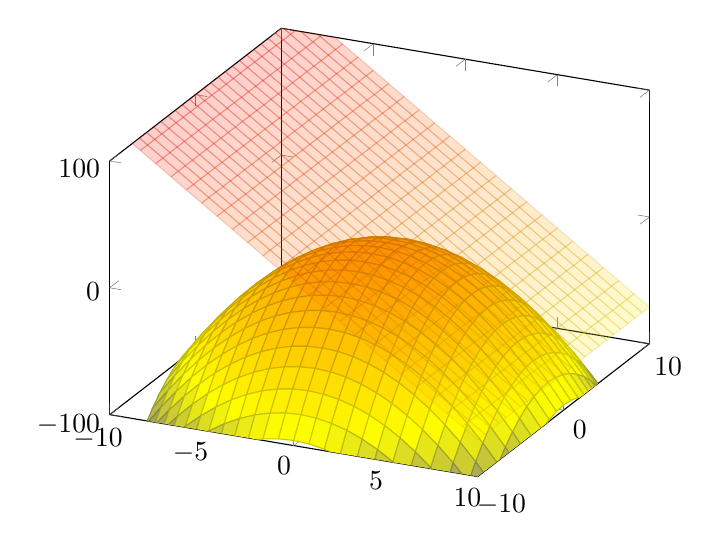
\begin{tikzpicture}
    \begin{axis}[xmin=-10,xmax=10,ymin=-10,ymax=10,zmin=-100,zmax=100]
    \addplot3[surf,domain=-10:10] {-x^2-y^2+4};
    \addplot3[surf,domain=-10:10,opacity=0.2] {-10*x+29};
  \end{axis}
\end{tikzpicture}\\
$f(\begin{pmatrix} x \\ y \end{pmatrix}) \simeq ax + by +c$ \\ 
$f(x,y) \simeq f(x_0,y_0) + f_x (x_0,y_0)(x-x_0) + f_y(x_0,y_0)(y-y_0)$
\begin{prz} 
    $f(x,y) = 2x^2 + 3xy + y^3 \\ 
    f_x = 4x + 3y \\ 
    f_y = 3x + 3x^2$
\end{prz}
$f(x,y) \simeq f(x_0,y_0)
\begin{aligned}[t]
    &+ f_x(x_0,y_0) (x-x_0) \\
    &+ f_y(x_0,y_0) (y-y_0) \\ 
    &+ d (x-x_0)^2  \\ 
    &+ e (y-y_0)^2  \\ 
    &+ f (x-x_0)(y-y_0)
\end{aligned} $ \\ 
$ f_{xx} = 4 \\ f_{xy} = 3 \\ f_{yx} = 3 \\ f_yy = 6y$ \\
$\begin{pmatrix} 
    f_{xx} & f_{xy} \\ f_{yx} & f{yy} 
\end{pmatrix}$ \\ 
$f: \mathbb R^n \to R$\\ 
$\begin{pmatrix} 
    f_{x_1 x_1} & f_{x_1 x_2} & \ldots \\ 
        & \ddots & \\ 
        & & 
\end{pmatrix}$ 
\begin{prz} 
    $a x^2 + b xy + cy^2 = \begin{pmatrix} x & y \end{pmatrix}
    \begin{pmatrix} a & \frac{b}{2} \\ \frac{b}{2} & c \end{pmatrix} 
    \begin{pmatrix} x \\ y \end{pmatrix}$
\end{prz} 
\begin{prz} 
    $a x^2 + by^2 + cz^2 + dxy + eyz + fxz = 
    \begin{pmatrix} x & y & z \end{pmatrix} 
    \begin{pmatrix} a & \frac{d}{2} & \frac{f}{2} \\ 
                    \frac{d}{2} & b & \frac{e}{2} \\ 
                \frac{f}{2} & \frac{e}{2} & c \end{pmatrix} 
    \begin{pmatrix} x \\ y \\ z \end{pmatrix} $
\end{prz} 
\begin{df} 
    Forma dwulinoiwa na przestrzeni liniowej $V$, to dwulinoiwa funkcja $\phi: V \times 
    V \to K$
\end{df}
\begin{ft} 
    Niech $B = (b_1,\ldots,b_n)$ będzie bazą $V$, a $\phi: V \times V \to K$ formą
    dwuliniową. Wówczas \[ \phi(v,w) = ([v]_B)^\top A [w]_B\] gdzie $A = (a_{ij}) 
    \in M_{n \times n} (K) \ a_{ij} = \phi(b_i,b_j)$. \\ 
    Macierz A oznaczamy $m^{BB}(\phi)$ i nazywamy macierzą formy dwuliniowej $\phi$ 
    w bazie $B$.
\end{ft} 
\begin{dd} $v_i,w_i \in K, b_i \in V$ \\ 
    $[v]_B = \begin{pmatrix} v_1 \\ \vdots \\ v_n \end{pmatrix},\ 
     [w]_B = \begin{pmatrix} w_1 \\ \vdots \\ w_n \end{pmatrix}$ \\ 
    $\phi(v,w) = \phi( \sum\limits_i v_i b_i, \sum\limits_j w_j b_j) = 
    \sum\limits_i \sum\limits_j v_i w_j \phi (b_i,b_j) = 
    \begin{pmatrix} v_1 &\dots& v_n \end{pmatrix}
    \begin{pmatrix} \phi(b_1,b_1) & \dots & \phi(b_1,b_n) \\ 
                    \vdots & \vdots & \vdots \\ 
                \phi(b_n,b_1) & \dots & \phi(b_n,b_n) \end{pmatrix}
    \begin{pmatrix} w_1 \\ \vdots \\ w_n \end{pmatrix}$
\end{dd}
\begin{ft} 
    $B = (b_1,\ldots,b_n) - $ baza przestrzeni liniowej $V$, zaś $A \in M_{n \times n}(K)$
    Wówczas \[ \phi(v,w) = ([v]_B)^\top A [w]_B\] jest formą dwuliniową.
\end{ft} 
\begin{dd} ~\\ 
    $\phi(\alpha_1 v_1 + \alpha_2 v_2,w) = ([\alpha_1 v_1+\alpha_2 v_2]_B)^\top 
    A[w]_B = (\alpha_1([v_1]_B)^\top + \alpha_2([v_2]_B)^\top)A [w]_B = 
    \alpha_1 \phi(v_1,w) + \alpha \phi(v_2,w)$ Analogicznie dla drugiej współrzędnej. 
\end{dd} 
\begin{ft} 
    $V - $ przestrzeń liniowa \\ 
    $B, C $ bazy $V$ \\ 
    $\phi: V \times V \to K$ forma dwulinowa 
    \[ m^{CC} (\phi) = (m_{\cancel{B}}^C(id))^\top m^{\cancel{B}\bcancel{B}}
    (\phi) (m_{\bcancel{B}}^C(id)) = P^T m^{BB}(\phi) P\]
\end{ft} 
\begin{dd} 
    $\phi (v,w) = ([v]_B)^\top m^{BB}(\phi) [w]_B = (m_B^C(id)[v]_C)^\top m^{BB}(\phi) 
    (m_B^C(id)[w]_C) = \\ ([v]_C)^\top 
    \underbrace{((m_B^C (id))^\top m^{BB}(\phi) m_B^C(id))}_{m^{CC}(\phi)} [w]_C$
\end{dd} 
\begin{df} 
    Dwuliniowa forma $\phi: V \times V \to K$ jest: \\ 
        symetryczna, jeśli $(\forall v,w \in V) \phi(v,w) = \phi(w,v)$ \\ 
        antysymetryczna, jeśli $(\forall v,w \in V) \phi(v,w) = - \phi(w,v)$
\end{df} 
\begin{ft} 
    Forma dwuliniowa $\phi$ jest (anty)symetryczna iff $m^{BB} (\phi)$ jest 
    (anty)symetryczna w pewnej (=dowolnej) bazie $B$. 
\end{ft} 
\begin{dd} ~\\ 
    $\phi(v,w) = ([v]_B)^\top A [w]_B$ \\ 
    $\phi(w,v) = (([w]_B)^\top A [v]_B)^\top = ([v]_B)^\top A^\top [w]_B$
\end{dd} 
\begin{df} 
    Funkcję $Q: V \to K$ nazywamy \underline{formą kwadratową} jeśli $Q(v) = \phi(v,v)$ 
    dla pewnej formy dwuliniowej $\phi$. (oznaczamy: $Q = \widetilde \phi$)
\end{df} 
\begin{prz} 
    $Q: \mathbb R^2 \to \mathbb R \ Q(\begin{pmatrix} x \\ y \end{pmatrix}) = ax^2 +bxy+ 
    cy^2 = \begin{pmatrix} x & y \end{pmatrix} \begin{pmatrix} a & \frac{b}{2} \\ 
    \frac{b}{2} & c \end{pmatrix} \begin{pmatrix} x \\ y \end{pmatrix}$
\end{prz} 
forma dwuliniowa $\phi \longrightarrow$ forma kwadratowa $Q(v) = \phi(v,v)$
\begin{uw} Jeśli $\phi,\phi'$ to formy dwuliniowe, $A = m^{BB}(\phi),\ A'=m^{BB}
(\phi)$ \\ 
$\forall i,j (a_{ij} + a_{ji} = a'_{ij} + a'_{ji})$, to $\widetilde\phi = \widetilde
{\phi}\, '$
\end{uw} 
\begin{uw} Od tej pory $\operatorname{char} K \neq 2$ \end{uw}
\begin{uw} $Q: V \to K$ forma kwadratowa \\ 
    $Q(v) = ([v]_B)^\top A [v]_B$, dla pewnej macierzy $A \in M_{n \times n}(K)$
    $B = (b_1,\ldots,b_n)$ - baza $V$. \\ 
    $a_{ii} = Q(b_i) = \phi(b_i,b_i)$
    $i \neq j \ a_{ij} = \phi(b_i,b_j)$ \\ 
    $Q(v+w) = \phi(v+w,v+w) = \phi(v,v)+\phi(v,w)+\phi(w,v)+\phi(w,w) = Q(v)
    + Q(w) + 2\phi(v,w)$
    czyli $a_{ij} = \frac{1}{2} (Q(b_i+b_j) - Q(b_i) - Q(b_j))$
\end{uw} 
\begin{ft}[wzór polaryzacyjny] 
    \[ \phi(v,w) = \frac{1}{2} (Q(v+w) - Q(v) - Q(w)) \]
    Dla dowolnej formy kwadratowej $Q = \widetilde \phi$ o ile $\phi$ symetryczne. 
\end{ft}
\begin{wn} 
    forma dwuliniowa symetryczna $\phi \longleftrightarrow$ forma kwadratowa $Q(v) = 
    \phi(v,v)$ \hfill (bijekcja)
\end{wn} 
\begin{uw} 
    Dla uproszczenia często używamy tego samego oznaczenia dla formy kwadratowej oraz 
    symetrycznej formy dwuliniowej od której ona pochodzi
\end{uw} 
\begin{ft} 
    Funkcja $Q: V \to K$ jest formą kwadratową iff spełnia obydwa warunki:
    \begin{enumerate}[(1)]
        \item $\phi(v,w) := \frac{1}{2} (Q(v+w) - Q(v) - Q(w))$ jest formą dwulinową. 
        \item $\forall t \in K \ \forall v \in V ( Q(tv) = t^2 Q(v))$
    \end{enumerate} 
\end{ft} 
\begin{dd} 
    \begin{itemize} \hfill
        \item[$\Downarrow$] \begin{enumerate}[(1)] 
                                \item wzór polaryzacyjny 
                                \item $Q(tv) = \phi(tv,tv,)=t^2 \phi(v,v) = t^2 Q(v)$
                            \end{enumerate} 
        \item[$\Uparrow$] $\phi(v,w) = \ldots $ forma dwuliniowa \\ 
            chcemy $Q = \widetilde \phi$ \\ 
            $Q(v) \overset{?}{=} \phi(v,v)$ \\ 
            $\phi(v,v) = \frac{1}{2} (Q(2v)-2Q(v)) \overset{2}{=}Q(v)$
    \end{itemize} 
\end{dd} 
\begin{tw}[o diagonalizacji formy kwadratowej] 
    $Q: V \to K$ forma kwadratowa \\ 
    Wówczas istnieje taka baza w przestrzeni $V$, że $m^{BB}(Q)$ jest diagonalna.\\
    (tzn. $Q(v) = \alpha_1 v_1^2 + \alpha_2 v_2^2 + \ldots + \alpha_n + v_n^2$ dla 
    $[v]_B = \begin{pmatrix} v_1 \\ \vdots \\ v_n \end{pmatrix}$)
\end{tw} 
\begin{dd} 
    $Q(x_1,\ldots,x_n) = \sum\limits_{i \le j} a_{ij} x_i x_j$ \\ 
    \underline{\textbf{Metoda Lagrange'a}} 
    \begin{enumerate}[(1)]
        \item Jesli $a_{ii} \neq 0$, dla pewnego $i$ b.s.o $i = 1$ \\ 
            $a_{11}x_1^2 + a_{12}x_1x_2 + \ldots a_{1n}x_1x_n + \sum\limits_{2 \le i \le j
                \le n} a_{ij}x_ix_j = a_{11}\underscript{(x_1 + \frac{a_{12}}{2a_{11}}x_2 + 
            \ldots + \frac{a_{1n}}{2a_{11}} x_n)^2}{\verteq\text{def}}{x'1} +
            \sum\limits_{2 \le i \le j \le n} a_{ij} x_i x_j = a_{11} (x'_1)^2 + 
            \sum\limits_{2 \le i \le j \le n} $ Dalej indukcyjnie. 
        \item Jeśli $a_{ii} = 0$ dla każdego $i$ to znajdujemy $a_{ij} \neq 0$ i 
            przeprowadzamy zamianę zmiennych $a_{ij}x_i x_j = 
            \frac{a_{ij}}{4} (\underscript{x_i + x_j}{\verteq}{x'_i})^2 - 
            \frac{a_{ij}}{4}(\underscript{x_i - x_j}{\verteq}{x'_j})^2 $
    \end{enumerate}
\end{dd}
od tej pory $K = \mathbb R$
\begin{df} 
    Formę kwadrotową $Q: V \to \mathbb R$ nazywamy: 
    \begin{itemize} 
        \item dodatnio określona jeśli $Q(v) > 0$ dla każdego $v \neq 0$ 
        \item ujemne określona, jesli $Q(v) < 0$ dla każdego $v \neq 0$ 
        \item dodatnio półokreślona $Q(v) \ge 0$ dla każdego $v \neq 0$ 
        \item ujemnie półokreślona $Q(v) \le 0$ dla każdego $v \neq 0$ 
    \end{itemize} 
\end{df} 
\begin{tw}[tw. Sylvestera] ~\\
    $Q: V \to \mathbb R$ forma kwadratowa \\ 
    $B -$ baza $V$ \\ 
    $m^{BB}(Q) = (a_{ij})_{1 \le i, j \le n}$ \\ 
    Wtedy $Q$ jest dodatnio określona $\Leftrightarrow$ $\det(a_{ij})_{1 \le i,j \le k}
    > 0$ dla $k = 1, 2, \ldots, n$
\end{tw} 
\begin{figure} 
    \centering
    \begin{tikzpicture}
        \draw (0,0) -- (5,0);
        \draw (0,0) -- (0,-5);
        \draw (1,0) -- (1,-1); 
        \draw (0,-1) -- (1,-1); 
        \draw (2,0) -- (2,-2); 
        \draw (0,-2) -- (2,-2);
        \draw (3,0) -- (3,-3); 
        \draw (0,-3) -- (3,-3); 
        \draw (5,0) -- (5,-5); 
        \draw (0,-5) -- (5,-5); 
        \draw [fill] (3.5,-3.5) circle[radius=0.025];
        \draw [fill] (4,-4) circle[radius=0.025];
        \draw [fill] (4.5,-4.5) circle[radius=0.025];
    \end{tikzpicture}
\caption{Ogólna idea tw Sylvestera, kolejne kwadraty oznaczają kolejne $(a_ij)_{1 \le i,j \le k} $ dla kolejnych $k$}
\end{figure} 
\begin{dd} \hfill
    \begin{itemize} 
        \item[$\Rightarrow$]$W = \operatorname{Lin} \{b_1,\ldots,b_k\} < V$ \\ 
                            $Q|_W: W \to \mathbb R$ dodatnio określona forma kwadratowa\\
                            Istnieje baza $C^{(k)}$, w której $Q|_W$ diagonalizowalna. \\
                            $B^{(k)}=(b_1,\ldots,b_n)$ \\ 
                            $m^{B^{(k)}B^{(k)}}(Q|_W)=(a_{ij})_{1 \le i,j\le k}=A^{(k)}$
                            $A^{(k)} = P^\top 
                            \begin{pmatrix} \lambda_1 & & \\ & \ddots & \\ & & \lambda_k
                            \end{pmatrix} P$ \\ 
                            $\lambda_1, \ldots,\lambda_k > 0$ \\ 
                            $\lambda_1 x_1^2 + \ldots + \lambda_k x_k^2 > 0$  
                            $\det(A^{(k)}) = \det P^\top \det P \lambda_1\dots\lambda_k=
                            (\det P)^2 \lambda_1 \dots \lambda_k > 0$
        \item[$\Leftarrow$]$\begin{aligned}[t] 
                            b'_k &= b_k - \sum\limits_{i =1}^{k-1} \frac{Q(b_k,bi')}{Q(
                            b_i',b_i')} b_i'\\ 
                            \vdots \\
                            b'_2 &= b_2 - \frac{Q(b_2,b_1')}{Q(b_1',b_1')} b'_1 \\
                            b'_1 &= b_1
                            \end{aligned}$ \\ 
                            Dowód indukcyjny następującego pakietu warunków: 
                            \begin{enumerate}
                                \item $\operatorname{Lin}\{b_1,\ldots,b_s\} = 
                                       \operatorname{Lin}\{b'_1,\ldots,b'_s\}$ 
                                \item $Q(b_s',b_s') > 0$ 
                                \item $Q(b_i',b_j') = 0$ dla $i \neq j,\ i j \le s$
                            \end{enumerate} 
                            $1^\circ$ oczywiste \\ 
                            $2^\circ$ 
                            \begin{itemize} 
                                \item[$(1)$]$\operatorname{Lin}\{b_1',\ldots,b_{s+1}'\}\ni
                                    \underbracket{b_1,\ldots,b_s}_{\text{zał indukcyjne}}
                                    b_{s+1} \leftarrow$ z defnicji $b_{s+1}$, czyli \\ 
                                    $\operatorname{Lin}\{b_1,\ldots,b_{s+1}\}= 
                                    \operatorname{Lin}\{b'_1,\ldots,b'_{s+1}\}$ 
                                \item[$(3)$] Dla $j \le s \ Q(b_j',b_{s+1}') = 
                                    Q(b_j',b_{s+1}) - \sum\limits_{i=1}^s
                                    \frac{Q(b_{s+1},b_i')}{Q(b_i',b_i')}b_i'=Q(b_j',b_{s+1
                                    })-\sum\limits_{i=1}^s \frac{Q(b_{s+1},b_i')}{Q(b_i',
                                    b_i')}Q(b_j',b_i')=Q(b_j',b_{s+1})-\frac{Q(b_{s+1},
                                    b_j')}{\cancel{Q(b_j',b_j')}} \cancel{Q(b_j',b_j')}=0$
                                \item[$(2)$] $m^{BB} (Q|_{\operatorname{Lin}\{b_1,\ldots,
                                    b_{s+1}\}})=A^{s+1} \\ 
                                    m^{B'B'}(Q|_{\operatorname{Lin}\{b'_1,\ldots,
                                    b'_{s+1}\}})=\begin{pmatrix} \lambda_1 & & 0 \\ 
                                    & \ddots & \\ 0 & & \lambda_{s+1}\end{pmatrix} 
                                    $ Ale wiemy $det A^{(s)} > 0$ \\ 
                                        $A^{(s+1)} = P^\top \begin{pmatrix} \lambda_1 & &
                                            \\ & \ddots & \\& &\lambda_{s+1}\end{pmatrix}
                                    \\ 0 < \det A^{(s)} = (\det P)^2 \lambda_1 \ldots 
                                    \lambda_s \lambda_{s+1}$ \\ czyli $\lambda_{s+1} > 0$
                                    \\ Zatem dla $B' = \{b_1',\ldots,b_n'\}$, to 
                                    $m^{B'B'}(Q) = \begin{pmatrix} \lambda_1 & & 
                                    \\ & \ddots & \\ & & \lambda_n \end{pmatrix}
                                    \lambda_1,\ldots,\lambda_n > 0$, czyli $Q$ dodatnie
                                    określone. 
                            \end{itemize} 
    \end{itemize} 
\end{dd} 

    \section{Iloczyn skalarny} 
\begin{df} 
    Iloczyn skalarny na rzeczywistej przestrzeni liniowej $V$, 
    to funckja $\langle \cdot, \cdot \rangle$: $V \times V \to \RR$, która jest 
    dwuliniową, symetryczną i dodatnio określoną forma. 
    \begin{enumerate}[(1)] 
        \item $\langle \alpha_1 v_1 + \alpha_2 v_2, w \rangle = 
            \alpha_1 \langle v_1, w \rangle + \alpha_2 \langle v_2, w \rangle$
        \item $\langle v, w \rangle = \langle w, v\rangle$ 
        \item $\langle v, v \rangle > 0 $ dla $v \neq 0$ 
    \end{enumerate} 
\end{df} 
\begin{df} 
    Przestrzeń euklidesowa to przestrzeń liniowa (rzeczywista) z iloczynem skalarnym. 
\end{df} 
\begin{df} 
    $V$ - przestrzeń euklidesowa 
    \begin{enumerate}[(1)]
        \item $|v| = \sqrt{ \langle v, v \rangle}$ (długość wektora)
        \item $\cos\sphericalangle(u,v) = \frac{\langle u, v \rangle}{|u||v|}$ (kąt 
            miedzy wektorami)
        \item $u \bot v \Leftrightarrow \langle u, v \rangle = 0$ (ortogonalnosć)
    \end{enumerate} 
\end{df} 
\begin{uw} ~\hfill
    \begin{enumerate}[(1)] 
        \item $|v| \in \RR_+$ dla $v \neq 0 \\
            |0| = 0 \qquad(\langle 0, 0 \rangle = \langle 0, \alpha 0 \rangle = \alpha 
            \langle 0 , 0 \rangle$ zatem $\langle 0, 0 \rangle = 0)$
        \item $| \langle u, v \rangle | \le |u| |v|$ 
    \end{enumerate} 
\end{uw} 
\begin{ft}[Nierówność Schwarza] \[ | \langle u, v \rangle | \le |u| |v| \] \end{ft} 
\begin{dd} ~\\ 
    $\langle u +tv, u +tv \rangle \ge 0 \quad t \in \RR$ \\ 
    $f(t) = \langle u,u \rangle + t^2 \langle v,v \rangle + 2t \langle u, v \rangle \ge 0,$
    $f: \RR \to \RR$ \\ 
    $\Delta \le 0$ \\
    $(2 \langle u,v \rangle)^2 - 4 |u|^2 |v|^2 \le 0$ \\ 
    $ \langle u,v \rangle )^2 \le (|u||v|)^2 $ \\ 
    $ |\langle u, v \rangle| \le |u| |v|$ \hfill \qed
\end{dd} 
\begin{ft}[Nierwność trójkąta] 
    \[ |u+v| \le |u| + |v| \]
\end{ft} 
\begin{dd} 
    $|u+v|^2 = \langle u+v, u+v \rangle = \langle u, u \rangle + \langle v, v \rangle + 
    2 \rangle u, v \langle = |u|^2 + |v|^2 + 2 \langle u, v \rangle \overset{\text{Schwarz}
    }{\le} |u|^2 + |v|^2 + 2|u||v| = (|u| + |v|)^2$ \hfill \qed
\end{dd} 
\begin{wn} ~\\ 
    $V$ - przestrzeń euklidesowa \\ 
    Wówczas $d(u,v) := |u-v|$ jest metryką na $V$. 
\end{wn} 
\begin{dd} \hfill 
    \begin{enumerate}[(1)] 
        \item $|u-v| = |v-u| \\ 
            |-w| = \sqrt{\langle -w,-w \rangle} = \sqrt{\cancel{(-1)}\cancel{(-1)}
            \langle w, w \rangle } = |w|$
        \item $|u-v| + |v-w| \ge |u-w|$ \\ 
            Nierówność trójkąta dla $u-v$ i $v-w$. 
        \item $|u - v| < 0 $ dla $u \neq v \quad |0| = 0$ \\ 
            Dodatnia określonosć $\langle \cdot, \cdot \rangle$
    \end{enumerate} 
\end{dd}
\begin{przy} \hfill 
    \begin{enumerate}[(1)] 
        \item $\RR^n$ \\ 
            $\left \langle \begin{pmatrix} x_1 \\ \vdots \\ x_n \end{pmatrix}, 
                \begin{pmatrix} y_1 \\ \vdots \\ y_n \end{pmatrix} \right \rangle
            = \sum\limits_{i=1}^n x_i y_i$ (standardowy iloczyn na $\RR^n$)
        \item $\RR_n[x]$ \\ 
            $\langle P, Q \rangle = \int\limits_0^1 P(x) Q(x) dx$
        \item niestandardowy iloczyn skalarny na $\RR^n$ \\ 
            $\langle u, v \rangle = u^\top A v$, gdzie $A$ - symetryczna dodatnie określona
            macierz \\ 
            np. $A = \begin{pmatrix} 1 & 1 \\ 1 & 2 \end{pmatrix}$ \\ 
            $\left \langle \begin{pmatrix} x \\ y \end{pmatrix}, 
                     \begin{pmatrix} x' \\ y' \end{pmatrix} \right \rangle_A = 
                     \begin{pmatrix} x & y \end{pmatrix}
                     \begin{pmatrix} 1 & 1 \\ 1 & 2 \end{pmatrix}
                     \begin{pmatrix} x' \\ y' \end{pmatrix} = xx' + 2yy' + xy' + x'y$
        \item $C[0,1]$ \\ 
            $\langle f, g \rangle = \int\limits_0^1 f(x)g(x) dx$
    \end{enumerate} 
\end{przy} 
\begin{df} 
    $V$ - przestrzeń euklidesowa \\ 
    $A \subset V$ \\ 
    Dopełnieniem ortogonalnym $A$ nazywamy 
    \[ A^\bot = \{ v \in V: (\forall a \in A) (\scp av = 0)\}\]
\end{df} 
\begin{ft} \hfill 
    \begin{enumerate}[(1)] 
        \item $A^\bot < V$ 
        \item $A^\bot = (\Lin A)^\bot$
        \item $A \subset B \Rightarrow A^\bot \supset B^\bot$ 
        \item Jeśli $\dim V < \infty, \ W < V$, to $V = W \oplus W^\bot$
    \end{enumerate} 
\end{ft}
\begin{dd} \hfill 
    \begin{enumerate}[(1)] 
        \item $\begin{aligned} \scp a{v_1} = 0 \\ \scp a{v_2} = 0 \end{aligned}
            \Rightarrow \scp{a}{\alpha_1 v_1 + \alpha_2 v_2} = 0$
        \item $\supset$ z $(3)$ \\
              $\subset$ \\ 
              $ v \in A^\bot$ tzn $\scp av = 0 \quad \forall a \in V$ \\ 
              $\alpha_1 v_1 + \ldots \alpha_n v_n \in \Lin A,\ a_i \in A,\ \alpha_1 \in\RR
              \\ \scp v{\alpha_1 a_1 + \ldots + \alpha_n v_n} =
              \alpha_1 \underscript{\scp{v_1}{a_1}}{\verteq}{0} + \ldots +
              \underscript{\scp{v_n}{a_n}}{\verteq}{0} = 0$ 
        \item $\checkmark$
        \item $\underscript{W \cap W^\bot}{\vertni}{w} = \{0\}$, bo $\scp ww = 0$, czyli 
            $w = 0$ \\ 
            $b_1,\ldots,b_k$ - baza $W$ \\ 
            $F: V \to \RR^k$ liniowe $v \mapsto \begin{pmatrix} \scp v{b_1} \\ \vdots \\ 
            \scp v{b_n} \end{pmatrix}$ \\ 
            $\ker F = \{b_1,\ldots,b_n\}^\bot = W^\bot$ \\ 
            $\underscript{\dim V}{\verteq}{n} = \underscript{\dim\operatorname{Im}F}
            {\vertge}{k} + \underscript{\dim W^\bot}{\vertle}{n-k}$ \\ 
            $\dim W^\bot + \dim W \underset{=}{\ge} \dim V$ \hfill \qed
    \end{enumerate} 
\end{dd} 
\begin{df} 
    $V - $ przetrzeń euklidesowa $\dim V < \infty,\ W < V$ 
    Rzutem prostopadłym (ortogonalnym) na $W$ nazywamy odwzorowanie $P_W: V \to V$ 
    takie, że $P_W (v) = w$, gdzie $v = \underscript{w}{\vertni}{W} +
    \underscript{w^\bot}{\vertni}{W^\bot}$ to jednoznaczne takie przedstawienie. 
\end{df} 
\begin{ft} 
    $P_W$ jest liniowe
\end{ft} 
\begin{dd} ~\\ 
    $\begin{aligned}[t] 
        v_1 &= w_1 + w_1^\bot \\ 
        v_2 &= w_2 + w_2^\bot \\ 
        v_1 + v_2 &= \underscript{w_1+w_2}{\vertni}{W}+
        \underscript{w_1^\bot+w_2^\bot}{\vertni}{W^\bot}
    \end{aligned}$ \\czyli $P_w(v_1 + v_2) = w_1 + w_2= P_W (v_1) + P_W (v_2)$ (podobnie
    jednorodność)
\end{dd} 
\begin{ft} 
    Jeśli $W = \Lin\{W\}$, to $P_W(v) = P_w(v) = \frac{\scp vw}{\scp ww} w$
\end{ft} 
\begin{dd} 
    $v = \underscript{\frac{\scp vw}{\scp ww}}{\vertni}{W} w
    + (v- \underscript{\frac{\scp vw}{\scp ww}}{\vertin\; ?}{\underscript{W^\bot}{\verteq}
    {w^\bot}})$ \\ 
    $\scp w {v - \frac{\scp vw}{\scp ww}w} = \scp wv - \frac{\scp vw}{\cancel{\scp ww}}
    \cancel{\scp ww} = 0$
\end{dd} 
\begin{ft} 
    $P_W(v)$ to jedyny punkt minimalizujący odległość od $v$
\end{ft} 
\begin{dd} 
%piękny rysunek xD %%% twierdznie pitagorasa 
    $\begin{aligned}[t]
        (d(v,w))^2 = |v-w|^2 &= |(v - P_W(v)) + (P_W(v)-w)|^2 \\ 
                             &= \scp{(v-P_W(v))+(P_W(v)-w)}{(v-P_W(v))+(P_W(v)-w)} \\
                             &= |v - P_W(v)|^2 + |P_W(v)-w|^2 + 2\underscript
                             {\scp{v-P_W(v)}{P_W(v)-w}}{\verteq}{0}
    \end{aligned}$ \\
    czyli $|v-w|^2 \ge |v - P_W(v)|^2 \Leftrightarrow P_W(v) = w$
\end{dd} 
\begin{df} 
    $V -$ przestrzeń euklidesowa, $\dim V < \infty$ \\ 
    $B = (b_1,\ldots,b_n)$ - baza 
    $B$ nazywamy: 
    \begin{itemize}
        \item bazą ortogonalną, jeśli $\scp{b_i}{b_j} = 0$ dla $i \neq j$
        \item bazą ortonormalną (ON), jeśli 
            $\scp{b_i}{b_j} = \begin{cases} 0, & i \neq j \\ 1, & i = j \end{cases}$
    \end{itemize} 
\end{df} 
\begin{ft} 
    Każda skończonie wiele wymiarowa przestrzeń euklidesowa ma bazę ortonomrlaną
\end{ft} 
\begin{dd} [ortogonalizacja Grama-Schmidta] ~\\ 
    $b_1,\ldots,b_n$ - dowolona baza \\ 
    $\begin{aligned} 
        b_1' &= b_1 \\ 
        b_2' &= b_2 - P_{b_1'}(b_2) \\ 
        b_3' &= b_3 - P_{b_2'}(b_3)  - P_{b_1'}(b_3) = b_3 - P_{\Lin\{b_1',b_2'\}}(b_3)\\
             &\vdots \\ 
        b_k' &= b_k - P_{\Lin\{b_1',\ldots,b_{k-1}'\}}(b_k) = 
                b_k - \sum\limits_{i=1}^{k-1} P_{b_i'}(b_k)
    \end{aligned}$ \\
    Indukcja dla $j < k$: 
    $\scp{b_k'}{b_j'} = \scp{b_j'}{b_k - \sum\limits_{i=1}^{k-1} P_{b_i'} (b_k)} = 
    \scp{b_j'}{b_k} - \sum\limits_{i=1}^{k-1} \scp{b_j'}{\frac{\scp{b_k}{b_i'}}
    {\scp{b_i'}{b_i'}b_i'}} \overset{\text{zał ind.}}{=} \scp{b_j'}{b_k} - 
    \scp{b_j'}{\frac{\scp{b_k}{b_j'}}{\scp{b_j'}{b_j'}} b_j'} = 0$, czyli \\ 
    $b_1',\ldots,b_n'$ - parami ortogonalne \\ 
    Dodatkowo: 
    $\Lin\{b_1,\ldots,b_n\} = \Lin\{b_1',\ldots,b_n'\}$ prosta induckja, więc \\ 
    $b_1',\ldots,b_n'$ - baza ortogonalna \\ 
    $\frac{b_1'}{|b_1'|},\ldots,\frac{b_n'}{|b_n'|}$ - baza ortonormalna \\ 
    Ponadto \\ 
    $b_k = \underscript{b_k'}{\vertin}{\Lin\{b_1',\ldots,b_{k-1}'\}^\bot} + 
    \underscript{\sum\limits_{i=1}^{k-1} P_{b_i'} (b_k)}{\vertin}{\Lin\{b_1',\ldots,b_{k-1}
    \}}$, czyli \\ 
    $\sum P_{b_i} (b_k) = P_{\Lin\{b_1',\ldots,b_{k-1}'\}} (b_k)$
\end{dd} 
\begin{wn} 
    Jeśli $b_1,\ldots,b_k$ - baza ortogonalna $W$, to $P_W(v) = \sum\limits_{i=1}^k P_{b_i}
    (v)$
\end{wn} 
\begin{ft} 
    $V $ - przestrzeń euklidesowa, $\dim V < \infty$, to $(V,\scp \cdot \cdot )$ jest
    izomorficzne z $(\RR^n,\scp \cdot \cdot _{\text{st}})$ przez izomorfizm 
    zachowujący iloczyn skalarny. 
\end{ft} 
\begin{dd} 
    $B = (b_1,\ldots,b_n)$ - ortonormalna baza $V$ \\ 
    $F: V \to \RR^n \quad F$ liniowe $F(b_i) = e_i, F(v) = [v]_B$ \\ 
    $v = \sum \alpha_i b_i$ \\ 
    $v - \sum \alpha_i'b_i$ \\ 
    $\scp v{v'} = \scp{\sum\limits_i\alpha_i b_i}{\sum\limits_j\alpha_j b_j} = 
    \sum\limits_i\sum\limits_j \alpha_i\alpha_j \scp{b_i}{b_j} = \sum\limits_i \alpha_i
    \alpha_i' = \scp{\begin{pmatrix} \alpha_1 \\ \vdots \\ \alpha_n \end{pmatrix}}
    {\begin{pmatrix} \alpha_1' \\ \vdots \\ \alpha_n' \end{pmatrix}}_{\text{st}}$
\end{dd} 

\begin{df} 
    $V $- przestrzeń liniowa nad $\CC$ 
    Zespolonym iloczynem skalarnym nazywamy funckję $\scp \cdot \cdot : V \times V 
    \to \CC$ takie, że 
    \begin{enumerate}[(1)] 
        \item $\scp{v_1+v_2}{w} = \scp{v_1}w + \scp{v_2}w$ \\ 
            $\scp{\alpha v}{w} = \alpha\scp wv$ \\ 
            $\scp{v}{w_1+w_2} = \scp{v}{w_1}+\scp{v}{w_2}$ \\ 
            $\scp{v}{\alpha w} = \overline{\alpha} \scp vw$ 
        \item $\scp{v}{w} = \overline{\scp vw}$ 
        \item $\scp vv \in \RR_+$ dla $v \neq 0$
    \end{enumerate} 
    \rule{3cm}{0.4pt} \\ 
    \footnotesize
    { 
        jeżeli $\scp \cdot \cdot$ spełnia
        \begin{itemize} 
            \item (1) jest formą 1,5 - liniową 
            \item (1) i (2) jest formą hermitowską 
            \item wszystkie to jest zespolonym iloczynem skalarnym
        \end{itemize} 
    } 
\end{df} 
$\scp {iv}{iv} = i\overline{i}\scp vv = \scp vv$
\begin{uw} 
    Jeśli $\scp \cdot \cdot: \CC^n \times \CC^n \to \CC$ zespolony iloczyn skalarny, to 
    $ \scp \cdot \cdot |_{\RR^n \times \RR^n}$ jest rzeczywistym iloczynem skalarnym. 
\end{uw} 
\begin{prz} \hfill 
    \begin{itemize} 
        \item[$1_\RR$] $\RR^n, \ \scp{\begin{pmatrix} x_1 \\ \vdots \\ x_n \end{pmatrix}}
            {\begin{pmatrix} y_1 \\ \vdots \\ y_n \end{pmatrix}} = \sum x_i y_i$
        \item[$1_\CC$] $\CC^n, \ \scp{\begin{pmatrix} x_1 \\ \vdots \\ x_n \end{pmatrix}}
            {\begin{pmatrix} y_1 \\ \vdots \\ y_n \end{pmatrix}} = \sum x_i\overline{y_i}$ 
        \item[$2_\RR$] $C[0,1] = \{ f:[0,1] \to \RR, f \text{ciągła} \} \\ 
            \scp f g = \int\limits_0^1 f(x) g(x) dx$
        \item[$2_\CC$] $C[0,1] = \{ f:[0,1] \to \CC, f \text{ciągła} \} \\ 
            \scp f g = \int\limits_0^1 f(x) \overline{g(x)} dx$
    \end{itemize} 
\end{prz} 
\begin{uw} 
    Prawie wszystko to co powiedzieliśmy (rzut ortogonalny, ortogonalność, 
    metoda Grama-Schmidta, nierówność Schwarza) 
    aplikuje się do zaespolonego iloczynu skalarnego. 
\end{uw} 
\textbf{Zadanie domowe} \\ 
Przeczytać wszystkie dzisiejsze dowody i znaleźć miejsca, które nie adaptuja się do 
przypadku zespolonego.

    \section{Twierdzenie spektralne}
\begin{tw}[spektralne] \hfill
  \begin{itemize}
    \item[$\RR$] Każda macierz symetryczna $(A^\top = A)$ macierz $A \in M_{n \times n}(\RR)$
    diagonalizuje się w pewnej bazie ortonormalnej i wszystkie jej wartości
    własne są rzeczywiste.
    \item[$\CC$] Każda samosprzężona (tzn $\underscript{\overline A^\top}
    {\verteq \text{ozn}}{A^*} = A$) macierz $A \in M_{n \times n}(\CC)$ diagonalizuje
    się w pewnej bazie ortonormalnej i wszystkie jej wartości własne są
    rzeczywiste.
  \end{itemize}
\end{tw}

\begin{prz} ~\\
  $\begin{pmatrix} 1 & 2 \\ 2 & 3 \end{pmatrix}^\top =
  \begin{pmatrix} 1 & 2 \\ 2 & 3 \end{pmatrix} \\
    \begin{pmatrix} 1 & 2+i \\ 2-i & 3 \end{pmatrix}^* =
      \begin{pmatrix} 1 & 2+i \\ 2-i & 3 \end{pmatrix}$
\end{prz}

\begin{ft} \hfill
  \begin{enumerate}[(1)]
    \item Jeśli $\scp{\cdot}{\cdot}$ jest standardowym (rzeczywistym) iloczynem
    skalarnym na $\RR^n$ to \[ \scp{Av}w = \scp v{A^\top w} \] dla dowolnych $v, w
    \in \RR^n,\ A \in M_{n \times n}(\RR)$
    \item Jeśli $\scp{\cdot}{\cdot}$ jest standardowym (zespolonym) iloczynem
    skalarnym na $\CC^n$ to \[ \scp{Av}{w} = \scp v{A^*w} \] dla dowolnych $v,w \in
    \CC^n,\ A \in M_{n \times n}(\CC)$
  \end{enumerate}
\end{ft}
\begin{dd} \hfill
  \begin{enumerate}[(1)]
    \item $\scp vw = v^\top w = \sum v_i w_i \\
           \scp{Av}w = (Av)^\top w = v^\top (A^\top w) = \scp v{A^\top w}$
    \item $\scp vw = \sum v_i \overline{w_i} = v^\top \overline w \\
           \scp{Av}w = (Av)^\top \overline w =
           v^\top \overline{\overline{A}^\top} \overline w =
           v^\top \overline{A^* w} = \scp{v}{A^* w}$
  \end{enumerate}
\end{dd}

\begin{wn} \hfill
  \begin{enumerate}[(1)]
    \item  Jeśli $A \in M_{n \times n}(\RR)$ i $A^\top = A$ to
    \[ \scp{Av}{w} = \scp{v}{Aw}\] dla dowolnych dla dowolnych $v,w \in \RR^n$
    \item Jeśli $A \in M_{n \times n}(\CC)$ i $A^* = A$, to
    \[ \scp{Av}{w} = \scp{v}{Aw}\] dla dowolnych $v,w \in \CC^n$
  \end{enumerate}
\end{wn}

\begin{dd}[tw. Spektralnego]
  $\lambda$ - wartość własna $A \quad \lambda \in \CC \ (A^* = A)$ \\
  $Av = \lambda v,\ v \neq 0$ \\
  $\lambda \scp{v}{v} = \scp{\lambda v}{v} = \scp{Av}v = \scp v{Av} =
  \scp v{\lambda v} = \overline \lambda \scp vv$, czyli \\
  $\lambda \scp vv = \overline \lambda \scp vv$, czyli $\lambda \in \RR$ \\
  Diagonalizacja $A$ przez indukcję ze względu na $n$:
  $\lambda_1$ - wartosć własna dla $A$ \\
  $Av_1 = \lambda_1 v_1,\ v_1 \neq 0$ \\
  $\RR^n = \Lin\{v_1\} \oplus \{v_1\}^\bot$ \\
  Cel: $\{v_1\}^\bot \quad F_A$ - niezmiennicza tzn.
  $\forall w \in \RR^n (\scp{w}{v_1} = 0 \Rightarrow \scp{Aw}{v_1} = 0)$ \\
  $\scp{Aw}{v_1} = \scp{w}{Av_1} = \scp{w}{\lambda_1 v_1} = \overline{\lambda_1}
  \scp{w}{v_1} = 0$ \hfill \qed
\end{dd}

\begin{df}[twierdznie]
  $A \in M_{n \times n}(\RR)$ nazywamy macierzą ortogonalną (lub macierzą
  izometrii) jeśli spełniony jest jeden/każdy z następujących warunków:
  \begin{enumerate}[(1)]
    \item kolumny $A$ stanowią bazę ortonormalną
    \item wiersze $A$ stanowią bazę ortonormalną
    \item $A^{-1} = A^\top$ (inaczej $A^\top A = AA^\top = I$)
    \item $F_A$ jest odwzorowaniem zachowującym iloczyn skalarny
    \item $F_A$ jest odwozorwaniem zachowującym długości (izometrią)
  \end{enumerate}
\end{df}
\begin{dd}
  $A = (v_1,\ldots,v_n)$ \\
  $(1) \Leftrightarrow \underscript{\scp{v_i}{v_j}}{\verteq}{v_i^\top v_j} =
  \begin{cases} 1, &i = j \\ 0, & i \neq j \end{cases} \Leftrightarrow
    \begin{pmatrix} v_1^\top \\ \vdots \\ v_n^\top \end{pmatrix}
    \begin{pmatrix} v_1 & \ldots & v_n \end{pmatrix} = I \Leftrightarrow (3)$ \\
  Podobnie $(2) \Leftrightarrow (3)$, czyli mamy $(1) \Leftrightarrow (2) \Leftrightarrow (3)$ \\
  $(4) \Leftrightarrow \scp vw = \scp{Av}{Aw} = \scp{v}{A^\top Aw}$ dla dowolnych
  $v,w \in \RR^n$ \\
  $A^\top A w = w$ dla każdego $w$ \\
  $A^\top A = I$ ($(4) \Rightarrow (3)$) \\
  $(3) \Rightarrow (4) \ A^\top A = I$ \\ 
  $\scp vw = \scp v{Iw} = \scp v{A^\top Aw} = \scp{Av}{Aw}$ \\ 
  $(4) \Rightarrow (5) \ |v| = \sqrt{\scp vv}$ \\
  $(5) \Rightarrow (4) \ \scp vw = \frac{1}{2} (|v + w|^2 - |v|^2 - |w|^2)$
\end{dd}

\begin{df}[twierdzenie] 
  $A \in M_{n \times n}(\CC)$ nazywamy macierzą unitarną, jeśli spełniony jest 
  jeden (=każdy) z następujących warunków
  \begin{enumerate}[(1)] 
    \item kolumny $A$ stanowią bazę ortonormalną $\CC^n$
    \item wiersze $A$ stanowią bazę ortonormalną $\CC^n$
    \item $A^{-1} = A^*$ (inaczej $A^* A = AA^* = I$)
    \item $F_A$ jest odwzorowaniem zachowującym iloczyn skalarny
    \item $F_A$ jest odwozorwaniem zachowującym długości (izometrią)
  \end{enumerate} 
\end{df} 
\begin{dd} analogiczny \end{dd} 
\begin{wn}{z tw. spektralnego} \hfill 
  \begin{enumerate}[(1)] 
    \item $A \in M_{n \times n}(\RR),\ A^\top = A$, to $A = PDP^{-1} = PDP^\top$ 
    ,gdzie $D$ - diagonalna ($D \in M_{n \times n}(\RR)$) 
    $P$ - ortogonalna
    \item $A \in M_{n \times n}(\CC),\ A^* = A$, to $A = UDU^{-1} = UDU^*$ \\ 
    $D \in M_{n \times n}(\RR) !!!$ \\ 
    $U$ - unitarna 
  \end{enumerate} 
\end{wn} 
\section{Macierze prostokątne}
$A \in M_{m \times n}(\RR)$ \\ 
$AA^\top \in M_{n \times n}(\RR)$ \\
$(A^\top A)^\top = A^\top (A^\top)^\top = A^\top A$ \\ 
$(AA^\top)^\top = (A^\top)^\top A^\top = AA^\top$ \\ 
$A^\top A, AA^\top$ są symetryczne oraz dodatnio połokreślone \\
\rule{2cm}{0.4pt} \\
$Q$ - forma kwadratowa o macierzy $A$ \\ 
$Q(v) = v^\top A v =\scp v{Av}$ \\ 
$Q(v,w) = v^\top A w = \scp v{Aw}$ \\ 
$A^\top A$ jest dodatnio półokreslony, tzn. \\ 
$\underscript{\scp v{A^\top Av}}{\verteq}{\scp{Av}{Av}} \ge 0$ \\ 
Podobnie $AA^\top$ \\
\rule{2cm}{0.4pt} \\
Zatem wartości własne $AA^\top,\ A^\top A$ to nieujemne liczby rzeczywiste. 
\begin{tw}[rozkład SVD\footnote{singular value decomposition}]
    Dla dowolnej macierzy $A \in M_{m \times n}(\RR)$ istnieje rozkład 
    \[ A = U\Sigma V^\top\] 
    gdzie $ \left. \begin{array}{l}
    U \in M_{m \times m}(\RR) \\ V \in M_{n \times n}(\RR) \end{array}\right \}$ macierze ortogonalne \\ 
    $\Sigma \in M_{m \times n}(\RR) \ \Sigma = \begin{pmatrix} D \\ 0 \end{pmatrix}$ lub 
    $\Sigma = \begin{pmatrix} D & 0 \end{pmatrix}$, gdzie $D$ - diagonalna. \\
    Co więcej: 
    \begin{itemize}
    \renewcommand\labelitemi{--}
    \item niezerowe wyrazy $\Sigma$ są dodatnimi liczbami rzeczywistymi 
    \item kolumnami $U$ sa wektory własne $AA^\top$ 
    \item kolumnami $V$ są wektory własne $A^\top A$ 
    \item wyrazy na przekątnej $\Sigma$ to pierwiastki wartości własnych $A^\top A$
    \end{itemize}
\end{tw}
$A = \begin{pmatrix} u_1 & \ldots & u_n \end{pmatrix} 
\begin{pmatrix} \lambda_1 & & \\ & \ddots & \\ & & \lambda_n \\ & & & \\ & & & \end{pmatrix} 
\begin{pmatrix} v_1^\top \\ \vdots \\ v_n^\top \end{pmatrix} m > n$ \\ 
$ \lambda_1 u_1 v_1^\top + \ldots + \lambda_m u_m v_m^\top$ \\ 
bez starty ogólności $\lambda_1 \ge \lambda_2 \ge \ldots \ge \lambda_m \ge 0$
\begin{uw} 
    Jeśli macierz $A \in M_{m \times n}(\RR)$ chcemy przybliczyć macierzą rzędu $r << m, n$, to 
    najlepsze przybliżenie, to $A \simeq \lambda_1 u_1 v_1^\top + \ldots + \lambda_r u_r v_r^\top$
\end{uw} 
\begin{dd} ~\\
    $A^\top A \overset{\text{tw. spektralne}}{=} VDV^\top$ \\ 
    $V$ - ortogonalna \\ 
    $D$ - diagonalna, $D = \begin{pmatrix} \lambda_1 & & \\ & \ddots & \\ & & \lambda_n \end{pmatrix} 
    \lambda_i \in \RR_+ \cup \{0\}$ \\ 
    \rule{2cm}{0.4pt} \\ 
    $m = n$ oraz $\lambda_1,\ldots,\lambda_n > 0$ \\ 
    $A = (AVD^{-\frac{1}{2}})D^{\frac{1}{2}}V^\top = U\Sigma V^\top$ 
    gdzie $\begin{pmatrix} \lambda_1 & & \\ & \ddots & \\ & & \lambda_n \end{pmatrix}
    \overset{\text{ozn.}}{=} \begin{pmatrix} \lambda_1 & & \\ & \ddots & \\ & & \lambda_n \end{pmatrix}$\\
    $\Sigma = D^{\frac{1}{2}}$ \\ 
    $U = AVD^{-\frac{1}{2}}$ \\ 
    $U^\top U = (AVD^{-\frac{1}{2}})^\top AVD^{-\frac{1}{2}} = D^{-\frac{1}{2}}V^\top (A^\top A)V
    D^{-\frac{1}{2}} = D^{-\frac{1}{2}}(V^\top V)D(V^\top)D^{-\frac{1}{2}} = I$, czyli $U$ jest 
    ortogonalne.
\end{dd} 
\begin{tw}[rozkład SVD (wersja zespolona)]
    Dla dowolnej $A \in M_{m \times n}(\CC)$ istnieje rozkład $A = U\Sigma V^*$, gdzie $U, V$ - macierze 
    unitarne. \\
    $\Sigma = \begin{pmatrix} D \\ 0 \end{pmatrix}$ lub $\begin{pmatrix} D & 0 \end{pmatrix}$ \\ 
    gdzie $D$ jest diagonalną o nieujemnych rzeczywistach wyrazach na przekątnej. 
\end{tw} 
\begin{dd} analogiczny \end{dd} 
\subsection{Rozpoznawanie twarzy} 
$F^{(1)},\ldots,F^{(k)}$ - zdjęcia twarzy 
$\overline F = \frac{1}{k} \sum\limits_i F^{(i)}$ - średnia twarz \\ 
$\overline F^{(s)} = F^{(s)} - \overline F$ \\ 
$\overline F^{(s)} \in M_{m \times n}(\RR) \simeq \RR^{mn}$ \\ 
\begin{tikzpicture}[scale=0.5]
    \draw[->] (-12,0) -- (12,0) node[below]{$x$};
    \draw[->] (0,-6) -- (0,6) node[right]{$y$};
    \draw[->,thick] (-3,-3) -- (3,3) node[above]
        {kierunek w którym zbiór jest najbardziej rozproszony};
    \draw[fill] (0.4934858523654501,0.860518298508326) circle[radius=0.025];
    \draw[fill] (0.6638079607617523,0.19815942051416985) circle[radius=0.025];
    \draw[fill] (0.9308879903554367,0.8538904904043795) circle[radius=0.025];
    \draw[fill] (4.974315252850506,2.895189422697958) circle[radius=0.025];
    \draw[fill] (-2.4576669327864673,-0.4812591393908312) circle[radius=0.025];
    \draw[fill] (-0.1827234582095264,-1.6895847963414348) circle[radius=0.025];
    \draw[fill] (2.1836838055594106,2.902378306404439) circle[radius=0.025];
    \draw[fill] (-2.1537945864657444,-1.6643703685210747) circle[radius=0.025];
    \draw[fill] (5.033856078800751,3.960378379933209) circle[radius=0.025];
    \draw[fill] (0.7456581965210345,-2.253855012416922) circle[radius=0.025];
    \draw[fill] (7.266217688502848,4.864367285652897) circle[radius=0.025];
    \draw[fill] (0.9103782746960383,-0.1425217815313835) circle[radius=0.025];
    \draw[fill] (2.839275535937861,1.015473964555969) circle[radius=0.025];
    \draw[fill] (3.8830386583018695,2.2046007970511496) circle[radius=0.025];
    \draw[fill] (-3.986594928990235,-2.7510731038422453) circle[radius=0.025];
    \draw[fill] (-4.262861473155021,-2.2796593375337073) circle[radius=0.025];
    \draw[fill] (-3.418348420059692,0.12130341159320013) circle[radius=0.025];
    \draw[fill] (-2.7766926269083405,-2.7899371537491375) circle[radius=0.025];
    \draw[fill] (2.567203296237186,2.4566695616444685) circle[radius=0.025];
    \draw[fill] (-0.06511177990686884,1.1860552035291894) circle[radius=0.025];
    \draw[fill] (4.204469430329178,2.35465469708201) circle[radius=0.025];
    \draw[fill] (2.780453867204177,1.4895542873394116) circle[radius=0.025];
    \draw[fill] (-5.780961377189902,-3.514989713464555) circle[radius=0.025];
    \draw[fill] (0.958628893643957,2.1537887139744574) circle[radius=0.025];
    \draw[fill] (-0.7670041370598432,-0.20694754637033883) circle[radius=0.025];
    \draw[fill] (2.6865653144742794,2.6651875508655745) circle[radius=0.025];
    \draw[fill] (2.91390907393373,1.4875256085679425) circle[radius=0.025];
    \draw[fill] (3.550563040336469,1.9502677754954652) circle[radius=0.025];
    \draw[fill] (5.844799684982185,3.5151665210664444) circle[radius=0.025];
    \draw[fill] (-0.11849303815380102,-0.2944699909639642) circle[radius=0.025];
    \draw[fill] (4.780421543065727,2.4441954833370283) circle[radius=0.025];
    \draw[fill] (1.342199718723413,2.0339762610860554) circle[radius=0.025];
    \draw[fill] (-2.5691111120763828,-2.6314642883678845) circle[radius=0.025];
    \draw[fill] (-0.21783244909330185,-0.5456624898357506) circle[radius=0.025];
    \draw[fill] (0.5913296088808833,-1.5666958749421893) circle[radius=0.025];
    \draw[fill] (9.751211251623273,5.713412285970427) circle[radius=0.025];
    \draw[fill] (0.7977060847126889,-0.5674209260248292) circle[radius=0.025];
    \draw[fill] (-0.5740992259645354,-1.3359167384628412) circle[radius=0.025];
    \draw[fill] (3.861575002067515,3.0380221806075727) circle[radius=0.025];
    \draw[fill] (1.132152138012633,0.6167104309330096) circle[radius=0.025];
    \draw[fill] (-2.895284579535973,-2.795601178452311) circle[radius=0.025];
    \draw[fill] (-1.3965066200708909,-1.5669071022314445) circle[radius=0.025];
    \draw[fill] (0.2730620521254288,-1.4455755916354587) circle[radius=0.025];
    \draw[fill] (-9.525416457605019,-3.9043347997291846) circle[radius=0.025];
    \draw[fill] (-1.160849454268151,-1.5269052310158004) circle[radius=0.025];
    \draw[fill] (-3.8197950625500754,-3.119565326268457) circle[radius=0.025];
    \draw[fill] (-11.892183332910005,-5.439892835363576) circle[radius=0.025];
    \draw[fill] (0.14081105298112456,-0.39421801514711097) circle[radius=0.025];
    \draw[fill] (2.7678817583059727,-0.08806165759760232) circle[radius=0.025];
    \draw[fill] (-1.59414285501866,-0.48239584488453446) circle[radius=0.025];
    \draw[fill] (4.644418790065638,4.655691805228571) circle[radius=0.025];
    \draw[fill] (3.3438612282404705,-0.2231759309347574) circle[radius=0.025];
    \draw[fill] (1.3762655582061565,3.405703243633005) circle[radius=0.025];
    \draw[fill] (-4.076212909757563,-0.2162068171189413) circle[radius=0.025];
    \draw[fill] (-0.9781089986410438,-0.8785411407659105) circle[radius=0.025];
    \draw[fill] (-1.9527704686216012,-1.9395877287061447) circle[radius=0.025];
    \draw[fill] (-3.2181941344772387,-2.379878552069895) circle[radius=0.025];
    \draw[fill] (3.6051834336716557,0.8824351531227791) circle[radius=0.025];
    \draw[fill] (3.2141332138993275,1.0242107227612327) circle[radius=0.025];
    \draw[fill] (-0.03902223313640214,-0.23739994596425357) circle[radius=0.025];
    \draw[fill] (4.730572693532324,1.284981427773363) circle[radius=0.025];
    \draw[fill] (-4.154228714171534,-2.8538468489462825) circle[radius=0.025];
    \draw[fill] (0.9404062309432386,-1.199854859235778) circle[radius=0.025];
    \draw[fill] (-10.248656206713072,-5.1943994203144985) circle[radius=0.025];
    \draw[fill] (0.9791582210798115,1.912790057213526) circle[radius=0.025];
    \draw[fill] (-2.3324135758036304,-1.48985219775803) circle[radius=0.025];
    \draw[fill] (9.401628647666913,7.252009561782484) circle[radius=0.025];
    \draw[fill] (1.2593637883708488,3.2906105526652984) circle[radius=0.025];
    \draw[fill] (2.727452223815179,1.5898709419720134) circle[radius=0.025];
    \draw[fill] (6.9668206960338095,4.708663661344671) circle[radius=0.025];
    \draw[fill] (2.1895975209934244,-0.7994117126499718) circle[radius=0.025];
    \draw[fill] (2.6061680927306066,1.3022009982982075) circle[radius=0.025];
    \draw[fill] (-0.4271829744837792,1.152509796704273) circle[radius=0.025];
    \draw[fill] (0.4995627716686687,1.1462350413339912) circle[radius=0.025];
    \draw[fill] (3.7490394808713776,1.7998927181833189) circle[radius=0.025];
    \draw[fill] (1.484372035350263,-1.1511776321889946) circle[radius=0.025];
    \draw[fill] (-1.7921695905315964,1.0505727656733663) circle[radius=0.025];
    \draw[fill] (-3.6179867160574046,-2.377630744756578) circle[radius=0.025];
    \draw[fill] (5.472201114781904,0.8816425611954777) circle[radius=0.025];
    \draw[fill] (-1.9896024802938403,-1.4189025625194163) circle[radius=0.025];
    \draw[fill] (6.0637798332723065,2.4625583613707636) circle[radius=0.025];
    \draw[fill] (-7.790997545273577,-3.8048122699406193) circle[radius=0.025];
    \draw[fill] (5.406798423550952,0.6208255829113367) circle[radius=0.025];
    \draw[fill] (-4.524932039132841,-0.8112973218829862) circle[radius=0.025];
    \draw[fill] (-2.9728099927728637,-2.9249430356557893) circle[radius=0.025];
    \draw[fill] (-3.6854057154600213,-1.4318364581006504) circle[radius=0.025];
    \draw[fill] (-2.386918816150601,-1.7580096455218093) circle[radius=0.025];
    \draw[fill] (-6.550469013137169,-2.855390786438701) circle[radius=0.025];
    \draw[fill] (-4.042200850680477,-0.4110271230417408) circle[radius=0.025];
    \draw[fill] (-0.020293906179843946,-2.311148450130922) circle[radius=0.025];
    \draw[fill] (-2.501594200931024,-0.24939785085632216) circle[radius=0.025];
    \draw[fill] (1.105874927533934,0.20135638920924664) circle[radius=0.025];
    \draw[fill] (-3.351112466627758,-2.342348786648233) circle[radius=0.025];
    \draw[fill] (5.167360089558085,1.7934800345329065) circle[radius=0.025];
    \draw[fill] (-10.335781697491704,-5.552712819417305) circle[radius=0.025];
    \draw[fill] (-7.8172154680391674,-4.689421447604833) circle[radius=0.025];
    \draw[fill] (-5.016823748960661,-3.62207968322557) circle[radius=0.025];
    \draw[fill] (2.4503266858977724,0.3592677326600645) circle[radius=0.025];
    \draw[fill] (2.3663785502233017,1.3105983618922592) circle[radius=0.025];
    \draw[fill] (2.940309808409997,2.5193141327609685) circle[radius=0.025];
\end{tikzpicture}  \\
macierz kowariancji \\ 
$C = (c_{ij})$ \\ 
$c_{ij} = \frac{1}{k} \sum\limits_i \overline F_i^{(s)} \overline F_j^{(s)}$ \\ 
$\overline F^{(s)} = \begin{pmatrix} \overline F_1^{(s)} \\ 
    \vdots \\ F_mn^{(s)} \end{pmatrix} \leftarrow$ eigenvector \\ 
$C$ symetryczna \\
$F_1,\ldots,F_{100}$ - wektory własne dla największych wartości własnych , eigenfaces

    \section{Kompleksyfikacja} 
Ogólna idea: \\[0.25cm]
$\RR^n \to \CC^n$ \\ 
$M_{n \times n}(\RR) \to M_{n \times n}(\CC)$\\ 
$\RR \to \CC$ \\[0.5cm] 
Co dokładnie byśmy chcieli:\\[0.25cm]
$V - $ przestrzeń liniowa nad $\RR \to V_\CC - $ przestrzeń liniowa nad $\CC$ \\ 
$F: V \to V $ przekształcenie liniowe $\to F_\CC : V_\CC \to V_\CC$ \\ 
$V \subset V_\CC$ \\ 
jeśli $v,w \in V$, to $v +_\CC w = v + w$\\ 
jeśli $v \in V, \lambda \in \RR$, to $\lambda \cdot_\CC v = \lambda \cdot v$ \\ 
$F_\CC |_V = F$
\begin{df} 
    Kompleksyfikacją przestrzeni liniowej $V$ nad $\RR$ nazywamy przestrzeń liniową nad 
    $\CC$ zdefiniową następująco: 
    \begin{gather*} 
        V_\CC = \{ u + iv : u, v \in V \} \\ 
        (u + iv) + (u' + iv') = (u+u') + i(v +v') \\ 
        (a + ib) \cdot (u + iv) = (au - bv) + i(bu + av) \\ 
        a,b \in \RR,\ u,v \in V
    \end{gather*} 
\end{df} 
\begin{przy} ~\\
    Jeśli $V = \RR^n$, to $V_\CC = \CC^n$ \\ 
    Jeśli $V = \RR[x]$, to $V_\CC = \CC[x]$ \\ 
    Jesli $V = F(X,\RR)$, to $V_\CC = F(X,\CC)$
\end{przy} 
\begin{df} 
    Kompleksyfikacją przekształcenia liniowego $F: V \to V$ ($V - $ przestrzeń liniowa nad 
    $\RR$) nazywamy $F_\CC: V_\CC \to V_\CC$
    \[ F_\CC (u+iv) = F(u) + iF(v) \]
\end{df} 
\begin{ft} 
    $F_\CC$ jest $\CC - $ liniowe. 
\end{ft} 
\begin{dd} ~\\ 
    Należy sprawdzić addytywność: \\
    $F_\CC ((u+iv) + (u'+iv')) = F_\CC((u+u')+i(v+v')) = F(u+u') + iF(v+v') = 
    F(u) + F(u') + iF(v) + iF(v') = F_\CC (u+iv) + F_\CC(u' + iv')$ \\ 
    oraz jednorodność:  \\
    $F_\CC ((a+ib)(u+iv)) = F_\CC ((au-bv)+i(bu+av)) = F(au-bv)+iF(bu+av) = aF(u) - bF(v) 
    + ibF(u) + iaF(v) = a(F(u)+iF(v)) + ib(F(u)+iF(v)) = (a+ib) F_\CC (u+iv)$
\end{dd} 
\begin{ft} 
    Jeśli $b_1,\ldots,b_n \in V$ jest bazą $V$, to jest też bazą $V_\CC$
\end{ft} 
\begin{dd} ~\\ 
    generowanie: \\ 
    $V_\CC \ni u + iv = \sum \alpha_k + b_k + i\sum \beta_k + b_k = \sum (\alpha_k + 
    i \beta_k ) b_k$ \\ 
    lnz: $\sum (\alpha_k + i \beta_k) b_k = 0$ \\ 
    $ (\sum \alpha_k b_k) + i(\sum \beta_k b_k) = 0 \Rightarrow 
    \sum\alpha_k b_k = 0,\ \sum\beta_k b_k =0 \leftarrow$ a to już jest w $V$, czyli jedyna
    zerowa kombinacja liniowa jest $\forall k \ \alpha_k = \beta_k = 0 $
\end{dd} 
\begin{wn} $\dim_\CC (V_\CC) = dim_\RR (V)$ \end{wn} 
\begin{uw} $\dim_\CC (\CC^n) = n$, ale $\dim_\RR (\CC^n) = 2n$ \end{uw} 
\begin{wn} $V - $ rzecywista przestrzeń liniowa, $F: V \to V$ przekształcenie liniowe, to 
    $m_B^B (F) = m_B^B (F_\CC)$ \end{wn}
    \begin{df}[Fakt]
    Jeśli $(V,\scp \cdot \cdot) - $ przestrzeń euklidesowa (rzeczywista), to 
    $(V_\CC, \scp \cdot \cdot _\CC)$ jest przestrzenią euklidesową (zespoloną), gdzie:
    \[ \scp{u+iv}{u'+iv'}_\CC = \scp{u}{u'} + i\scp{v}{u'} - i\scp{u}{v'} + \scp{v}{v'}\]
\end{df} 
\begin{tw}[o postaci przekształcenia unitranego] ~\\
    Jeśli $U \in M_{n \times n} (\CC)$ jest unitarna, to $U = PDP^-1$, gdzie 
    $D - $ diagonalna, $P - $ unitarna. Wartości własne, co do modułu, sa równe $1$.
\end{tw} 
\begin{dd} był na ćwiczeniach \end{dd} 
\begin{tw}[o postaci przekształcenia ortogonalnego] ~\\ 
    Jeśli $A \in M_{n \times n}(\RR)$ jest ortogonalna, to 
    $A = P \begin{pmatrix} O_1 & & \\ & \ddots & \\ & & O_k \end{pmatrix} P^{-1}$, gdzie 
    $P$ - ortogonalna, a $O_i = \begin{pmatrix} \cos \theta_i & -\sin\theta_i
    \\ \sin \theta_i & \cos \theta_i \end{pmatrix}$ lub $O_i = (\pm 1)$
\end{tw} 
\begin{dd} ~\\ 
    $A \in M_{n \times n} (\RR)$ \\
    traktując $A$ jako macierz zespoloną dostajemy rozkład: 
    $A = P \begin{pmatrix} \lambda_1 & & \\ &\ddots& \\ & & \lambda_n \end{pmatrix}P^{-1}$
    \\$A = P \begin{pmatrix} 1 & & & & & & & & \\ 
                           & \ddots & & & & & & & \\ 
                           & & 1 & & & & & & \\ 
                           & & & -1 & & & & & \\ 
                           & & & & \ddots & & & &  \\ 
                           & & & & & -1 & & & \\ 
                           & & & & & & a_1 + ib_1 & & \\ 
                           & & & & & & & a_1 - ib_1 &  \\
                           & & & & & & & & \ddots 
           \end{pmatrix} P^{-1}$ \\ 
           $P=(\underbrace{b_1,\ldots,b_p}_{\text{dla} \pm 1},b_{p+1},\overline{b_p{+1}},\ldots)$ \\ 
        $\begin{pmatrix} & \\ u+iv & u - iv \\ & \end{pmatrix} 
        \begin{pmatrix} a + ib & \\ & a - ib \end{pmatrix} \begin{pmatrix} & \\ & 
    \end{pmatrix}^{-1}$ 
    $ \operatorname{Lin} \{u,v\} = \operatorname{Lin} \{b_{p+1}, \overline{b_{p+1}}\}$ \\ 
    $A (u+iv) = (a+ib)(u+iv)$ \\ 
    $A (u-iv) = (a-ib)(u-iv)$ \\ 
    $Au \pm Av = (au - bv) \pm i(bu+av)$ \\ 
    $Au = au - bv $ \\ 
    $Av = bu + av $ \\ 
    $\begin{pmatrix} a + ib & \\ & a - ib \end{pmatrix} 
    \to \begin{pmatrix} a & b \\ -b & a \end{pmatrix}$ \\ 
    $a^2 + b^2 = 1$, czyli $a = \cos \theta,\ b = -\sin\theta$
\end{dd} 
\begin{tw}[Jordana (wersja rzeczywista)] 
$A \in M_{n \times n}(\RR)$ \\ 
Wówczas $A = PJP^{-1}$, gdzie $J = \begin{pmatrix} J_1 & & \\ & \ddots & \\ & & J_n 
    \end{pmatrix}$, gdzie \\
    $J_i = \begin{pmatrix} \lambda_i \end{pmatrix},\ \lambda_i \in \RR$ \\ 
    lub \\ 
    $J_i = \begin{pmatrix} \lambda_i & 1 & & & \\ 
                           & \ddots & \ddots & & \\ 
                           & & \ddots & 1 &  \\
                           & & & \lambda_i 
    \end{pmatrix},\ \lambda_i \in \RR$ \\ 
    lub \\ 
    $J_i = 
    \begin{pmatrix} a_i & -b_i \\ b_i & a_i \end{pmatrix} a_i, b_i \in \RR$ \\ 
    lub \\
    $J_i = 
    \begin{pmatrix} 
        a_i & -b_i& 1      & 0      & &  \\ 
        b_i & a_i & 0      & 1      & &  \\ 
            & \ddots    &  & \ddots & &  \\ 
            &     &  \ddots  &  & 1 & 0 \\
            &     &        & \ddots& 0 & 1 \\ 
            &     &        & & a_i &  -b_i \\ 
            &     &        & & b_i & a_i
    \end{pmatrix}$ 
\end{tw} 
\begin{dd} 
    $A = PJP^{-1}$ - rozkład zespolony (dbając o to, by wektory bazowe dla rzeczywistych
    wartości własnych były rzeczywiste) \\ 
    $ \lambda \notin \RR$ \\ 
    $ \lambda, \overline \lambda$ \\ 
    $\overline {V_\lambda} = V_{\overline\lambda}$ \\ 
    $\overline{\ker (A-\lambda I)^n} = \ker (A - \overline\lambda I) \to $ klatka dla 
    $\lambda$ są takie same co dla $\overline \lambda$ \\ 
    Jeśli skonstruujemy kawałek bazy jordanowskiej $b_1,\ldots,b_n$ dla $\lambda$, to 
    $\overline b_1,\ldots,\overline b_n$ będą odpowiednio kawałekiem bazy jordanowskiej dla
    $\overline \lambda$. \\ 
    Następnie powtarzamy procedurę z poprzedniego twierdzenia. \\ 
    $b_1,\ldots,b_n,\overline b_1,\ldots,\overline b_n \to 
    \operatorname{Re} b_1, \operatorname{Im} b_1,\ldots,\operatorname{Re}b_n,
    \operatorname{Im} b_n$ 
\end{dd} 
\section{Objętość n-wymiarowa}
Znakowana objętosć $n-$wymiarowego równoległościanu rozpiętego przez wektory 
$v_1,\ldots,v_n \in \RR^n$
\begin{df}[tw] 
    Objętością $n-$ wymiarowego rownoległościanu rozpiętego przez $v_1,\ldots,v_n \in \RR^n$ 
    nazywamy każdą z poniżej podanych (równych) liczb. 
    \begin{enumerate}[(1)] 
        \item $|\det(v_1,\ldots,v_n)|$
        \item $V_n$, gdzie $\begin{cases} V_1 = |v_1| \\ 
                V_{k+1} = V_k * \operatorname{dist}
            (v_{k+1},\operatorname{Lin} \{v_1,\ldots,v_n \}) \end{cases}$
        \item $\sqrt{\det\begin{pmatrix} \scp{v_1}{v_1}&\ldots&\scp{v_1}{v_n} \\ 
                    & \vdots & \\ 
            \scp{v_n}{v_1} & \ldots & \scp{v_n}{v_n} \end{pmatrix}}$ macierz Grama
    \end{enumerate} 
\end{df} 
\begin{dd} ~
    \begin{itemize} 
    \item[$(1) \Leftrightarrow (3)$] 
        $\begin{pmatrix} \scp{v_1}{v_1} & \ldots & \scp{v_1}{v_n} \\ 
            & \vdots & \\ 
        \scp{v_n}{v_1} & \ldots & \scp{v_n}{v_n} \end{pmatrix} = 
        \begin{pmatrix} v_1^\top \\ \vdots \\ v_n^\top \end{pmatrix} 
        \begin{pmatrix} v_1 & \ldots & v_n \end{pmatrix} $ \\ 
        $G = A^\top A$ \\ 
        $\det G = \det A^\top \det A = (\det A)^2$
    \item[$(2) \Leftrightarrow (1)$] Zastosowanie ortogonalizacji Grama-Schmidta do $v_1,
        \ldots,v_n$ nie wpływa na wartość $V_n$.  \\ 
    Nie wpływa również na $\det(v_1,\ldots,v_n)$  \\ 
    Zatem wystarczy sprawdzić dla układu ortogonalnego. Wtedy: 
    $\det(v_1,\ldots,v_n) = (det(\scp{v_i}{v_j}))^{\frac{1}{2}} = \\ 
    \sqrt{|v_1|^2\ldots|v_n|^2} = |v_1|\ldots|v_n| = V_n$
    \end{itemize} 
\end{dd} 
\begin{wn} Objętość nie zależy od kolejności wektorów \end{wn} 
\begin{dd} Zamiana kolumn w macierzy $(v_1,\ldots,v_n)$ zmienia jedynie znak wyznacznika. 
\end{dd} 
\begin{wn} Objętość wynosi $|\det([v_1]_B,\ldots,[v_n]_B)|$, gdzie $B$ jest dowolną bazą 
ortonormalną \end{wn} 
\begin{dd} taki sam \end{dd} 
\begin{wn} $v_1,\ldots,v_n \in \RR^n$ lnz $\Leftrightarrow \det(\scp{v_i}{v_j}) \neq 0$
\end{wn} 
\section{Przestrzeń dualna} 
\begin{df} 
    $V - $ przestrzeń liniowa nad $K$ \\ 
    Przestrzenią dualną do $V$ nazywamy $V^* = \operatorname{Hom} (V,K)$ (elementy 
    $V^*$ nazywamy czasami funkcjonałami (liniowymi))
\end{df} 
\begin{ft} 
    Jesli $\dim V < \infty$, to $V^* \simeq V$
\end{ft} 
\begin{dd} 
    $b_1,\ldots,b_n - $ baza $V$ \\ 
    $b_1^*,\ldots,b_n^* \in V^*$ (baza dualna), $ b_i^* (b_j) = 
    \begin{cases} 1, & i = j \\ 0, & i \neq j \end{cases}$ \\
    Dalej rozszerzamy do liniowego $b_i^* V \to K$ \\ 
    (inaczej $b_i^* (\alpha_1 b_1 + \ldots + \alpha_n b_n) = \alpha_i$) \\ 
    generowanie: \\ 
    $v^* \in V^* \quad (v^* : V \to K)$ \\ 
    $ v^* \overset{?}{=} v^*(b_1) b^*_1 + \ldots v^*(b_n) b^*_n$ \\ 
    sprawdzimy, czy oba odwzorowania są zgodne na bazie $b_1,\ldots,b_n$  \\ 
    $v^* (b_j) = v^*(b_1) \underbracket{b_1^*(b_j)}_{0} + \ldots + 
    v^*(b_n) \underbracket{b_n^* (bj)}_{0}$ \\ 
    lnz: \\ 
    $\alpha_1 b-1 ^* + \ldots + \alpha_n b_n^* = 0$ \\ 
    $\alpha_1 b_1 ^* (b_j) + \ldots + \alpha_n b_n^*(b_j) = 0$ \\ 
    $\alpha_j = 0$ dla $j = 1,\ldots,n$ \\ 
    zatem $dim V^* = \dim V < \infty$, czyli $V^* \simeq V$ 
\end{dd} 
\begin{uw} ~\\  
    $V = \RR^\infty = 
     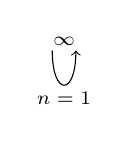
\begin{tikzpicture}[scale = 0.3,baseline]
        \node at (0.5,1.4) {\scriptsize$\infty$};
        \node at (0.5,-1) {\scriptsize$n=1$};
        \path[->] (0,1) edge [bend right = 90,looseness=5] (1,1);
    \end{tikzpicture} \  
    \RR^n$ \\ 
    $V^* \simeq V$ 
\end{uw} 
\begin{df} 
    $F: V \to W$ przekształcenie liniowe, to przekształcenie dualne do $F$, 
    to $F^*: W^* \to V^*$, takie, że $F^*(w^*) = w^* \circ F$
\end{df} 
\begin{ft} 
    Odwozorowanie $\varphi: V \to V^{**}$ zdefiniowane $\varphi(v)(f) = f(v)$ jest 
    monomorfizmem. W przypadku $\dim V < \infty $ jest to izomorfizm. 
\end{ft} 
\footnotetext{monomorfizm - różnowartościowe \\ epimorfizm - na \\ 
endomorifzm $V \to V$ \\ automirfozim = endo + izo}
$V^{**} = (V^*)^*$ 
$\varphi (v) \in (V^*)^*$ \\ 
$\varphi (v): V^* \to K$ \\ 
$\varphi (v) (f) = f(v)$ \\ 
$f: V \to K$

\end{document}
